\section{Data Quality Checks}

This section documents the basic data quality checks for ALEPH archieved data collected in the LEP1 and LEP2 period. In additional to the raw spectra from the data, jet and particle spectra are compared to the predictions from PYTHIA8 event generator (Version 8.230 Default Tune). 

\subsection{LEP1 vs LEP1 Monte-Carlo}
\begin{figure}[H]
\centering
\subfloat{\label{sfig:a}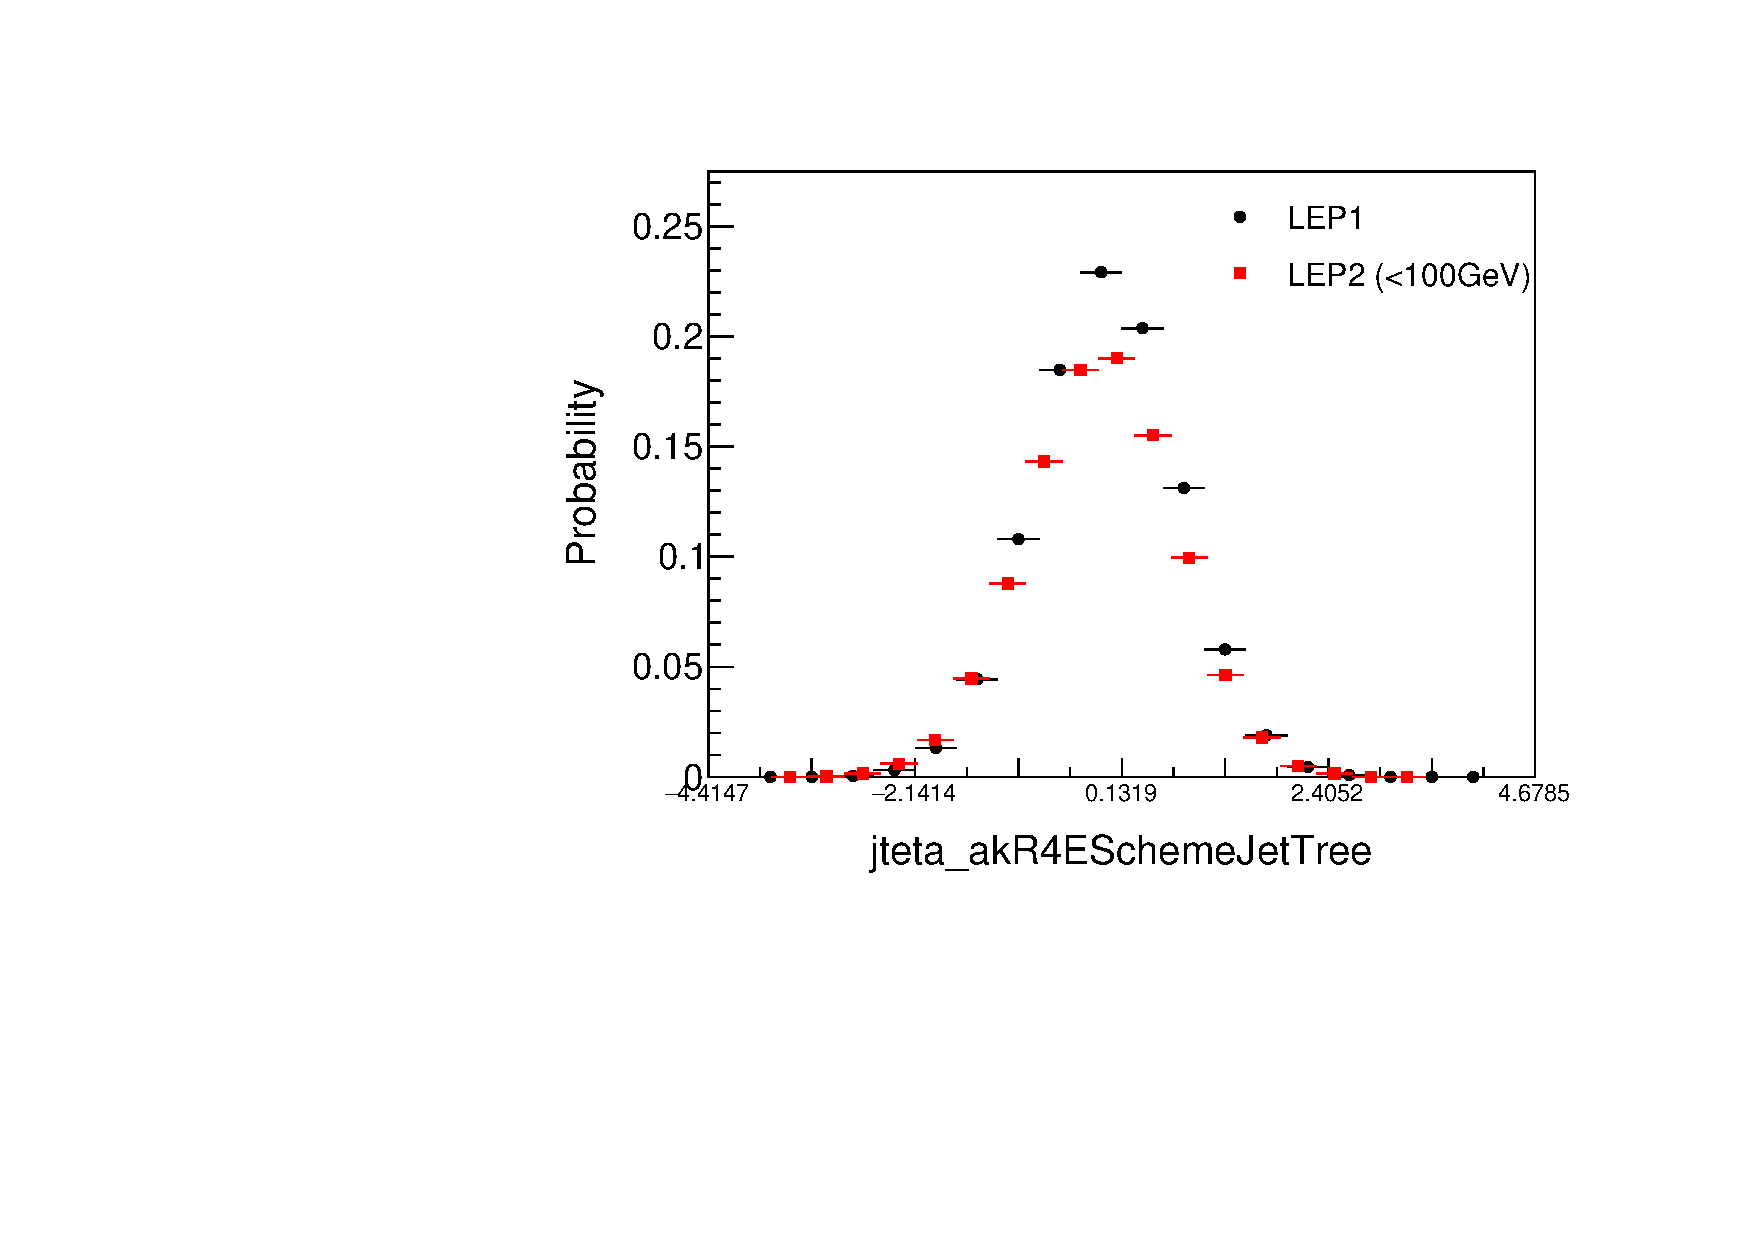
\includegraphics[width=.25\textwidth]{images/DQC/LEP1MC/jteta_akR4ESchemeJetTree.pdf}}\hfill
\subfloat{\label{sfig:b}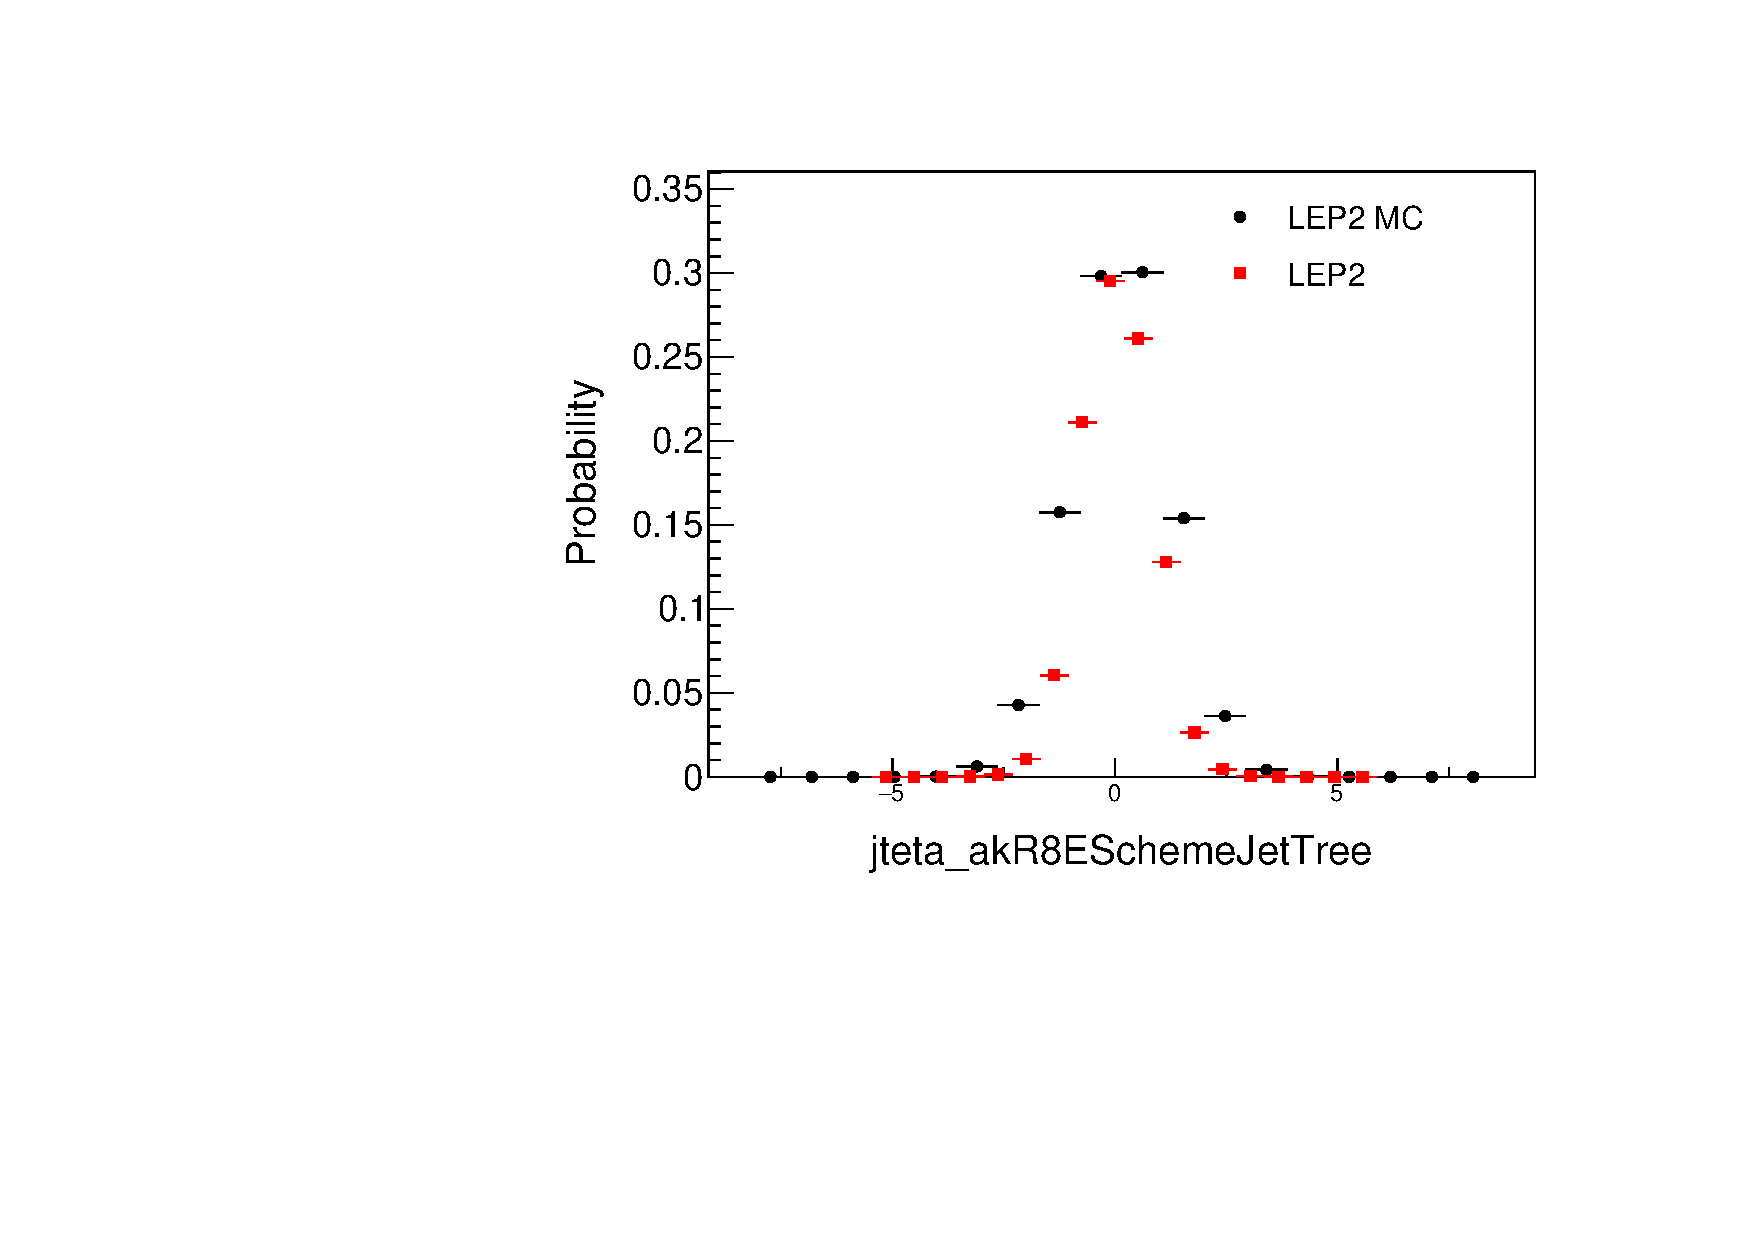
\includegraphics[width=.25\textwidth]{images/DQC/LEP1MC/jteta_akR8ESchemeJetTree.pdf}}\hfill
\subfloat{\label{sfig:c}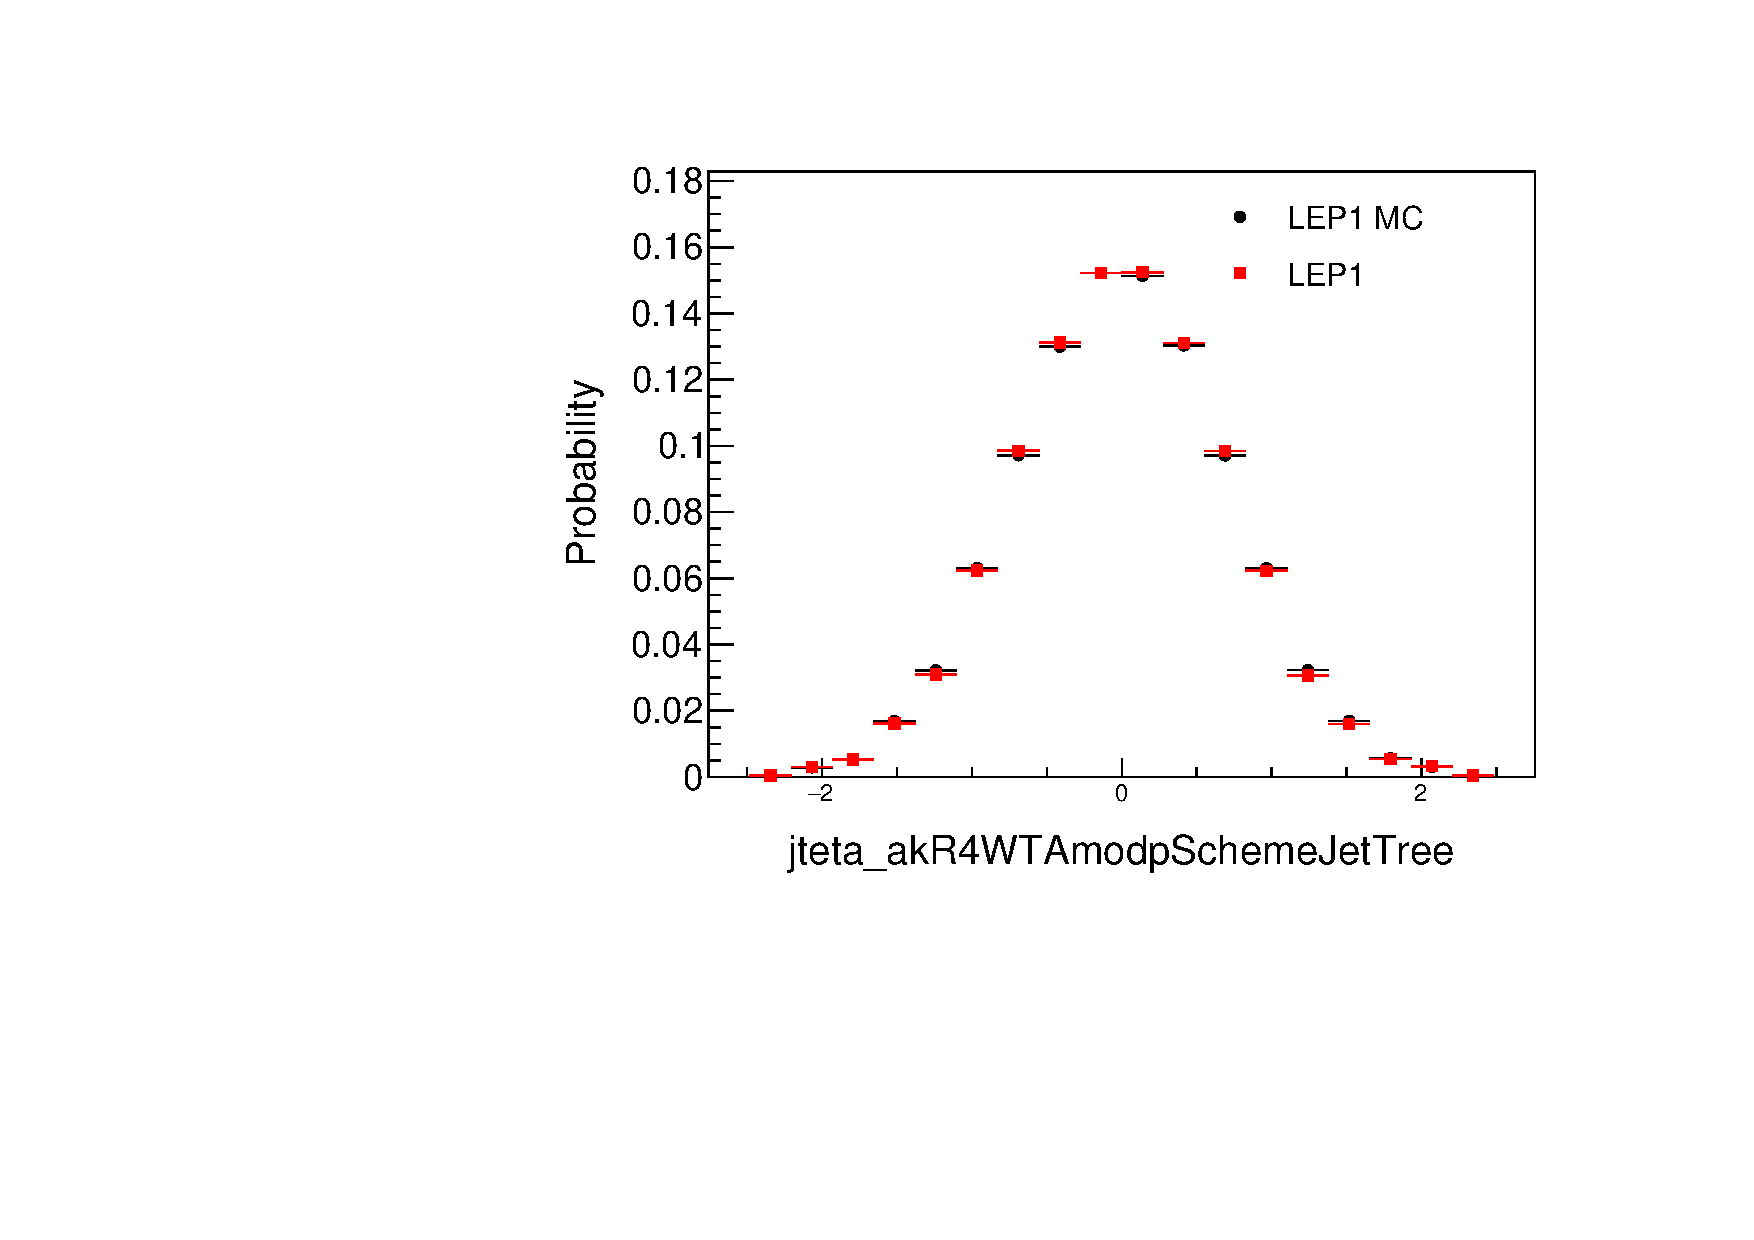
\includegraphics[width=.25\textwidth]{images/DQC/LEP1MC/jteta_akR4WTAmodpSchemeJetTree.pdf}}\hfill
\subfloat{\label{sfig:d}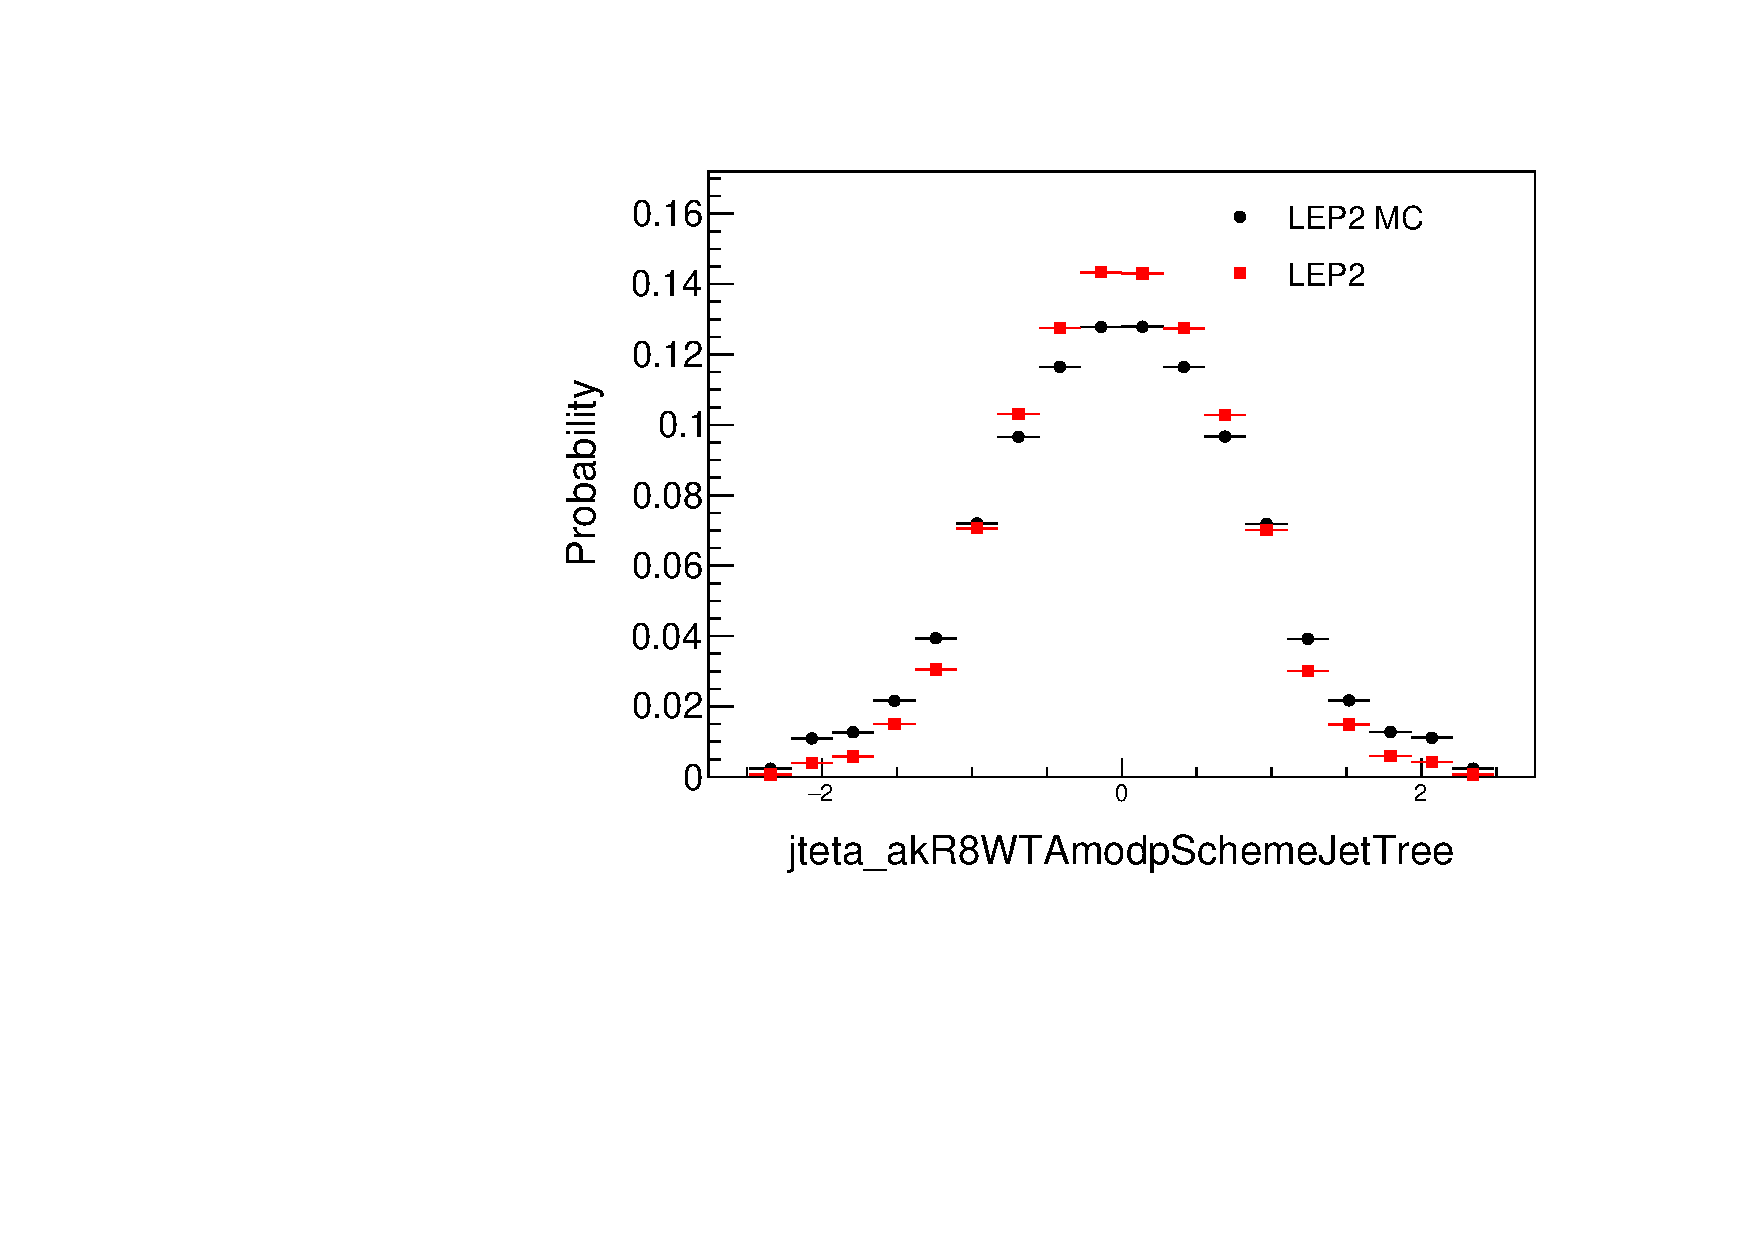
\includegraphics[width=.25\textwidth]{images/DQC/LEP1MC/jteta_akR8WTAmodpSchemeJetTree.pdf}}\hfill %row end
\subfloat{\label{sfig:e}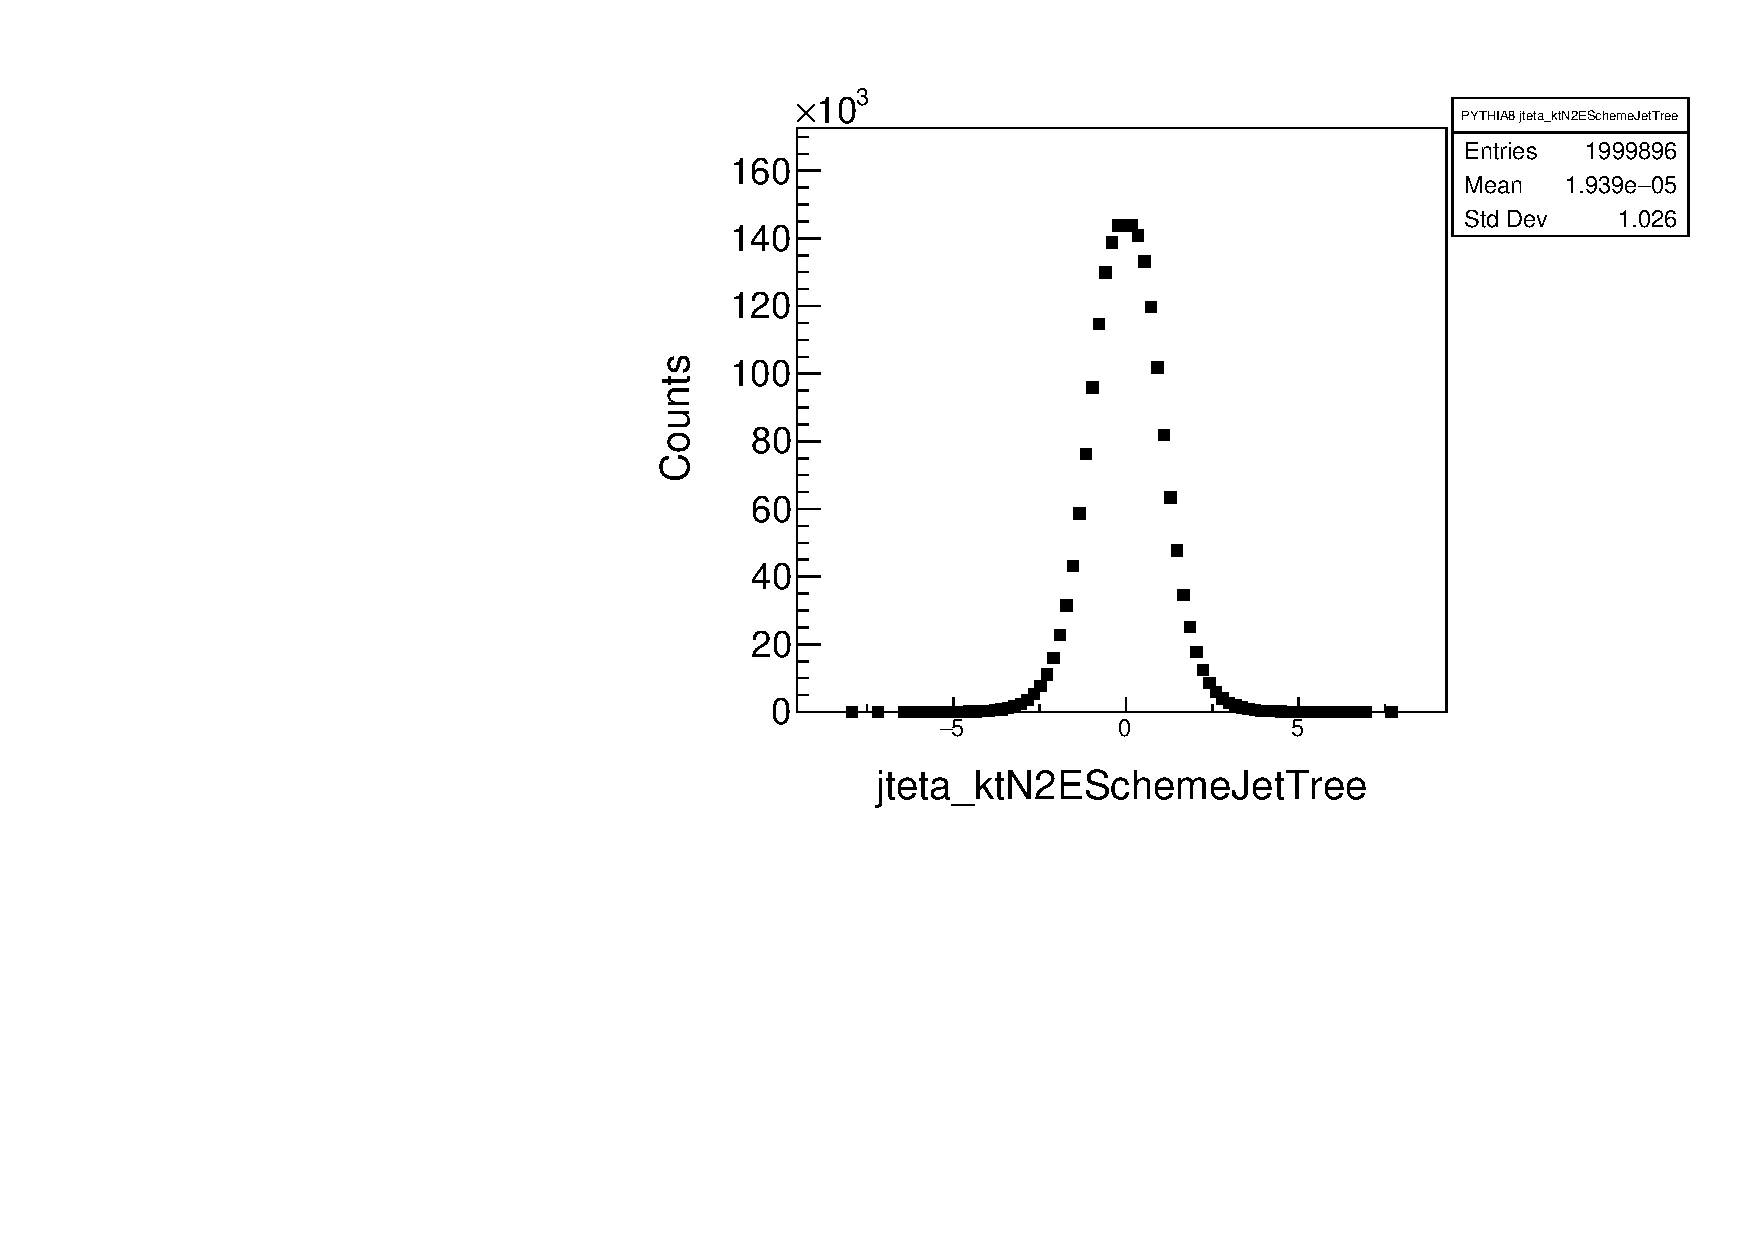
\includegraphics[width=.25\textwidth]{images/DQC/LEP1MC/jteta_ktN2ESchemeJetTree.pdf}}\hfill
\subfloat{\label{sfig:f}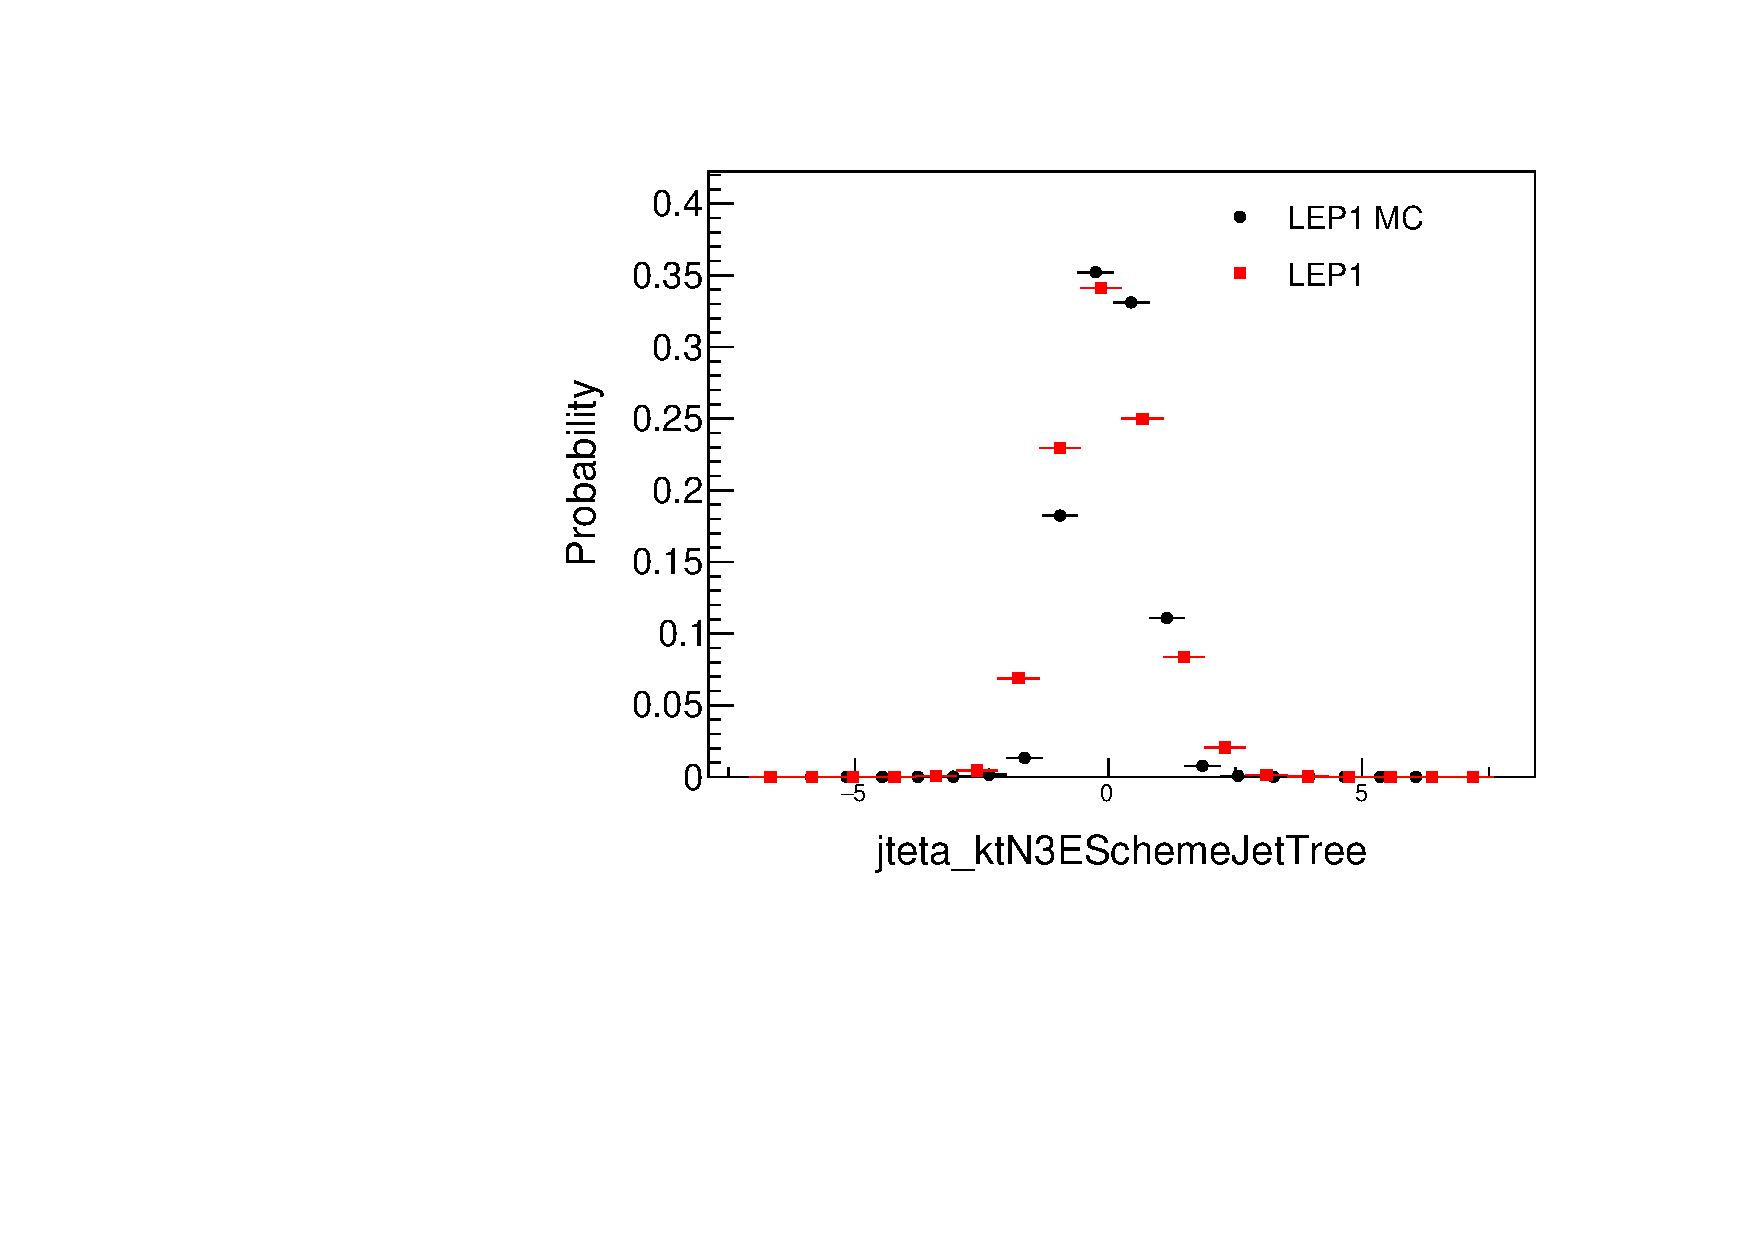
\includegraphics[width=.25\textwidth]{images/DQC/LEP1MC/jteta_ktN3ESchemeJetTree.pdf}}\hfill
\subfloat{\label{sfig:g}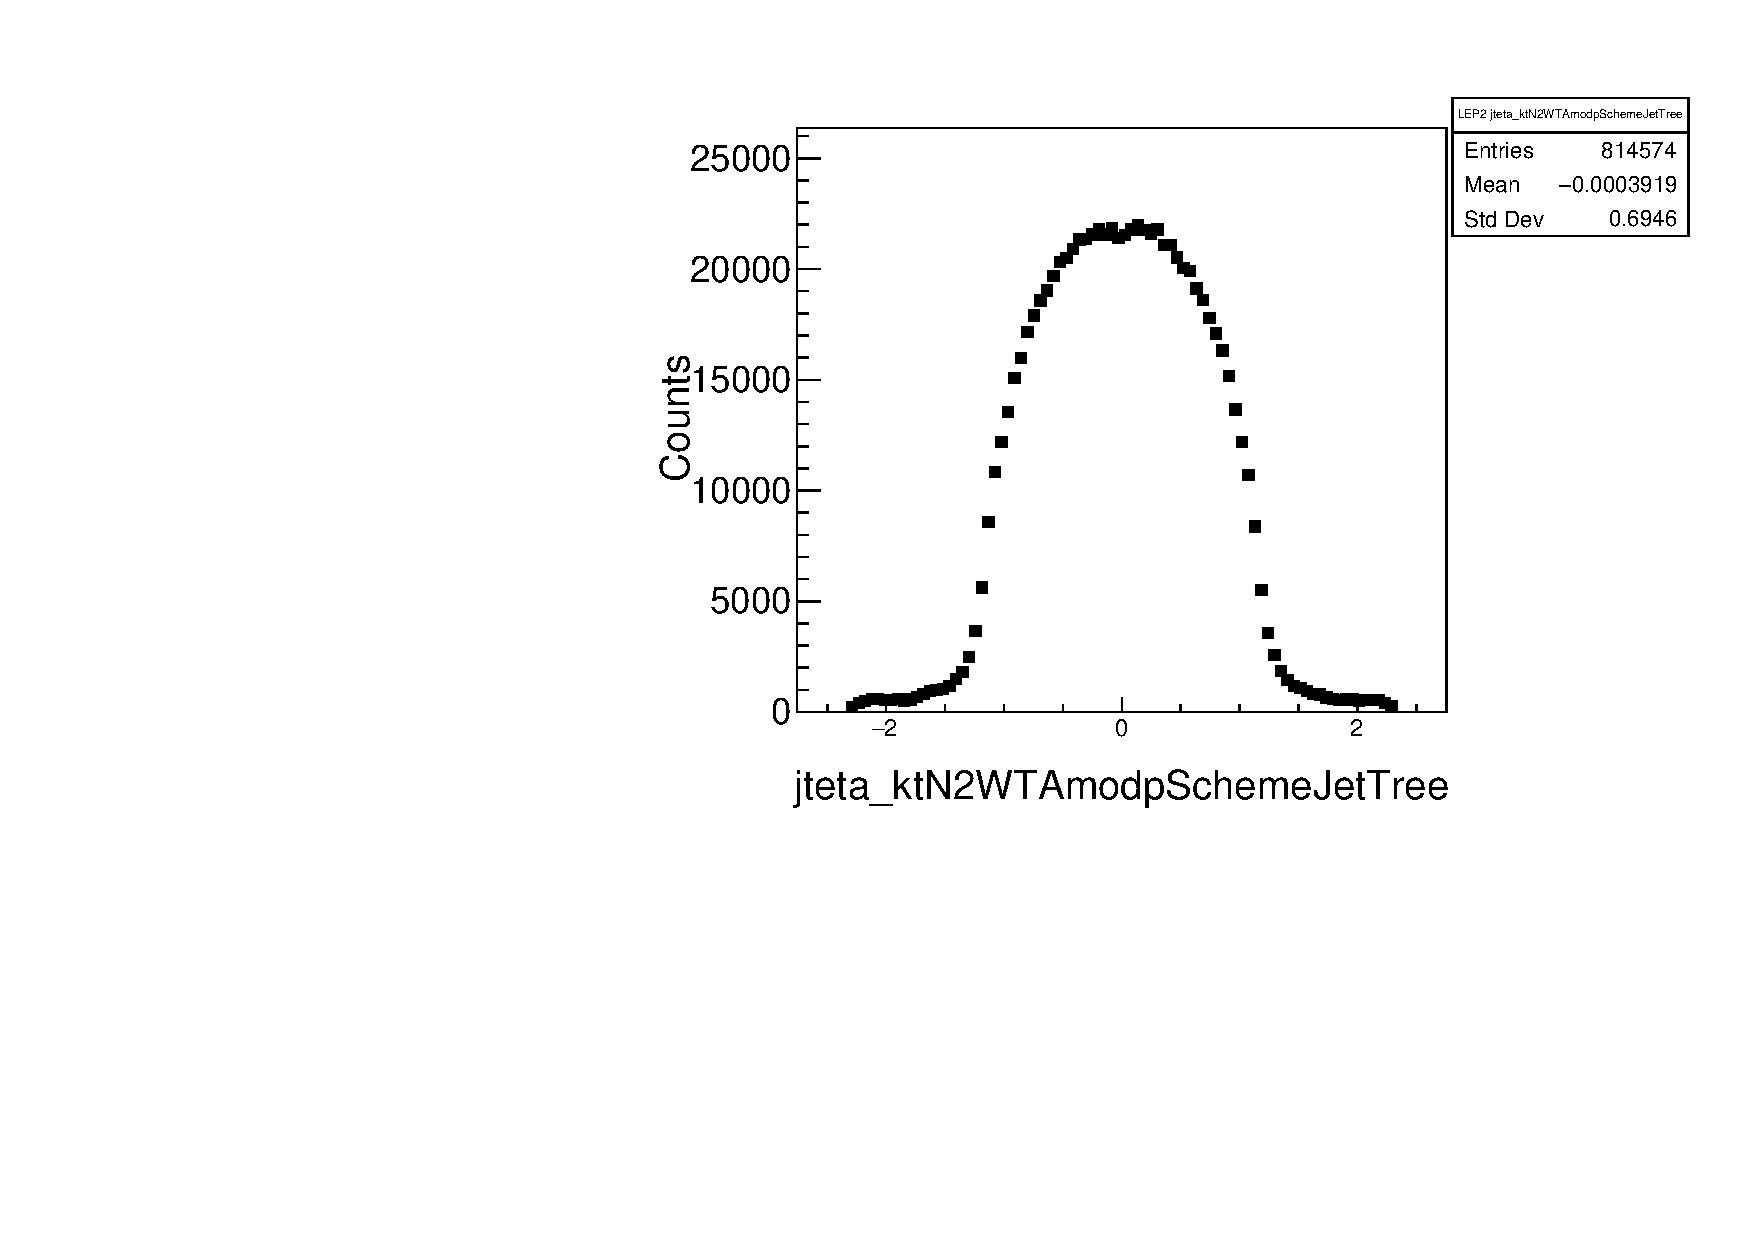
\includegraphics[width=.25\textwidth]{images/DQC/LEP1MC/jteta_ktN2WTAmodpSchemeJetTree.pdf}}\hfill
\subfloat{\label{sfig:h}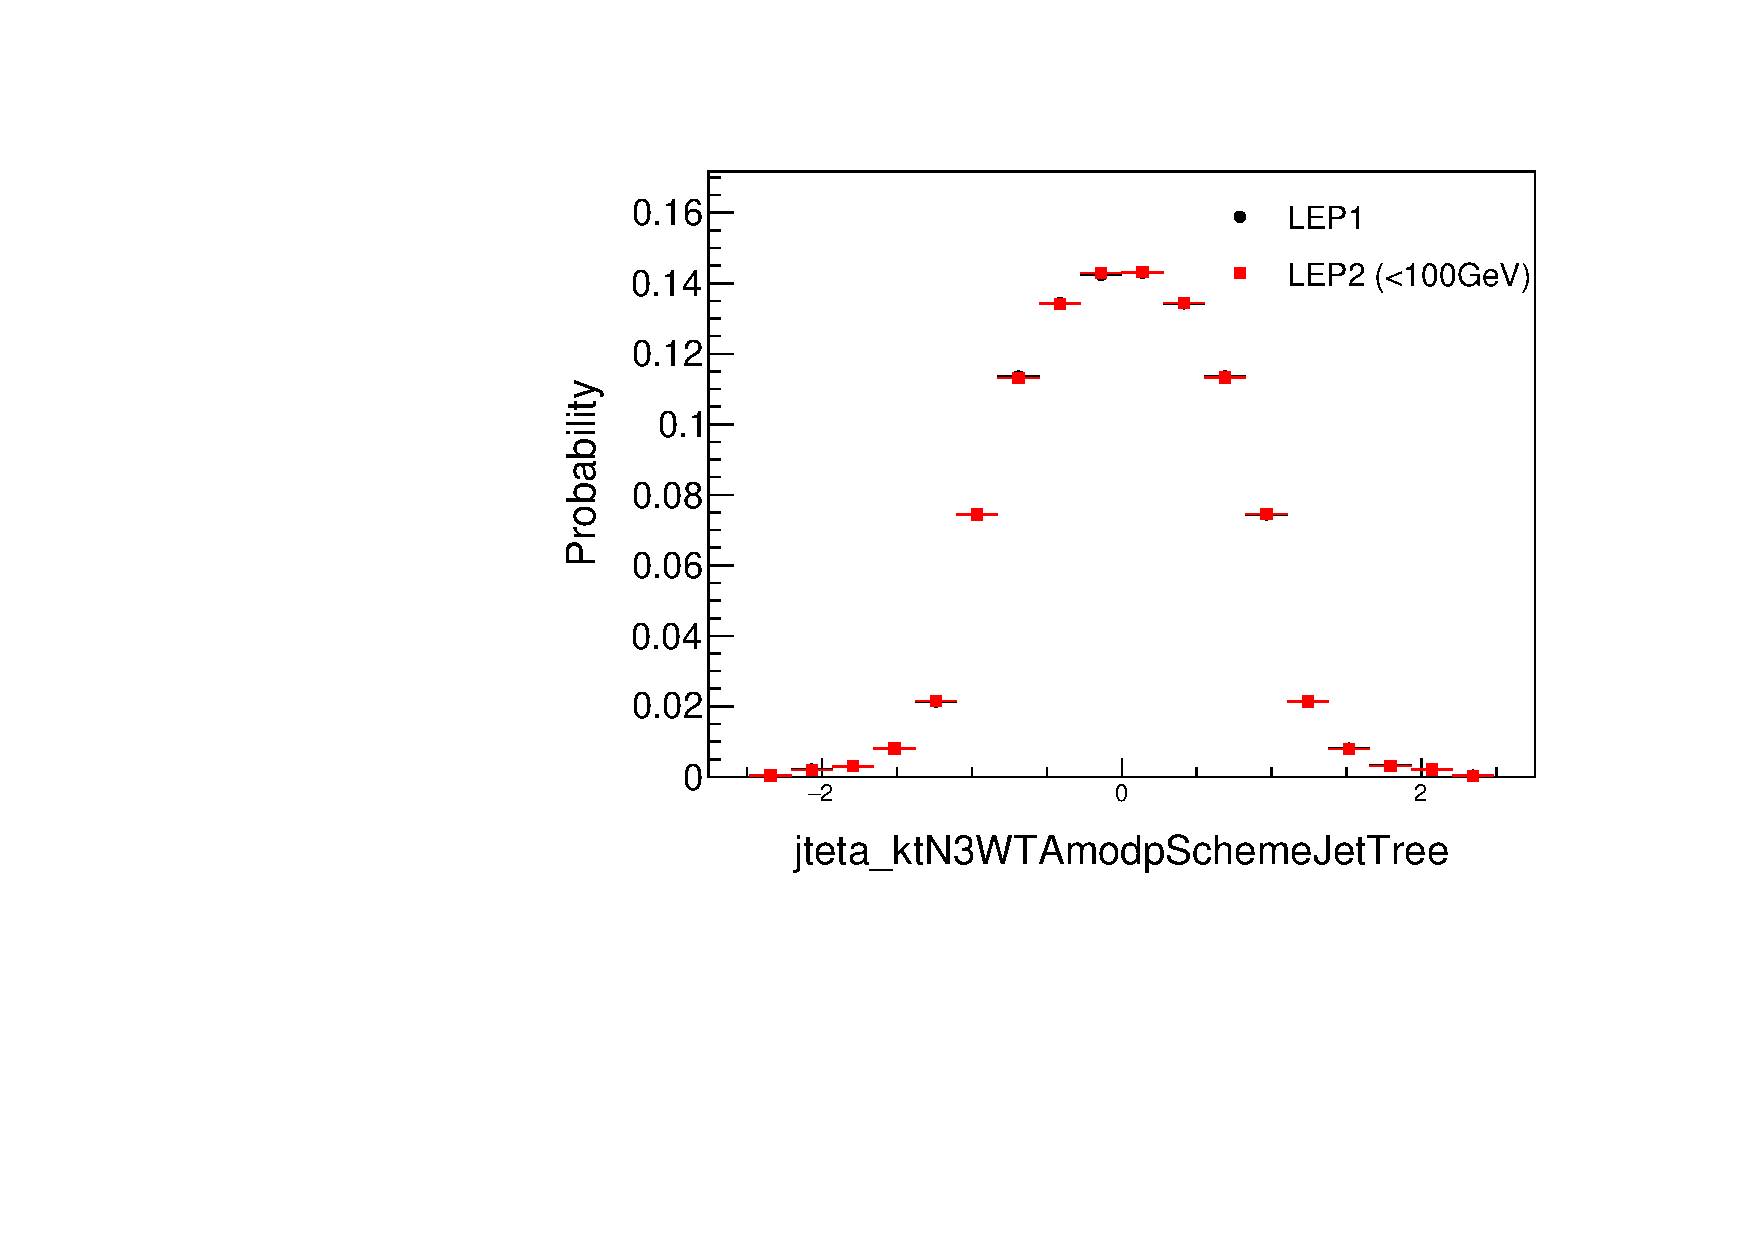
\includegraphics[width=.25\textwidth]{images/DQC/LEP1MC/jteta_ktN3WTAmodpSchemeJetTree.pdf}}\hfill
\caption{LEP1 vs LEP1 MC Jet $\eta$ distributions. Top row: anti-$k_t$, left to right: $R=0.4$, $E$ scheme; $R=0.8$, $E$ scheme; $R=0.4$, WTA mod p scheme; $R=0.8$, WTA mod p scheme. Bottom row: $k_t$, left to right: $N=2$, $E$ scheme; $N=3$, $E$ scheme; $N=2$, WTA mod p scheme; $N=3$; WTA mod p scheme.}  
\end{figure}

\begin{figure}[H]
\centering
\subfloat{\label{sfig:a}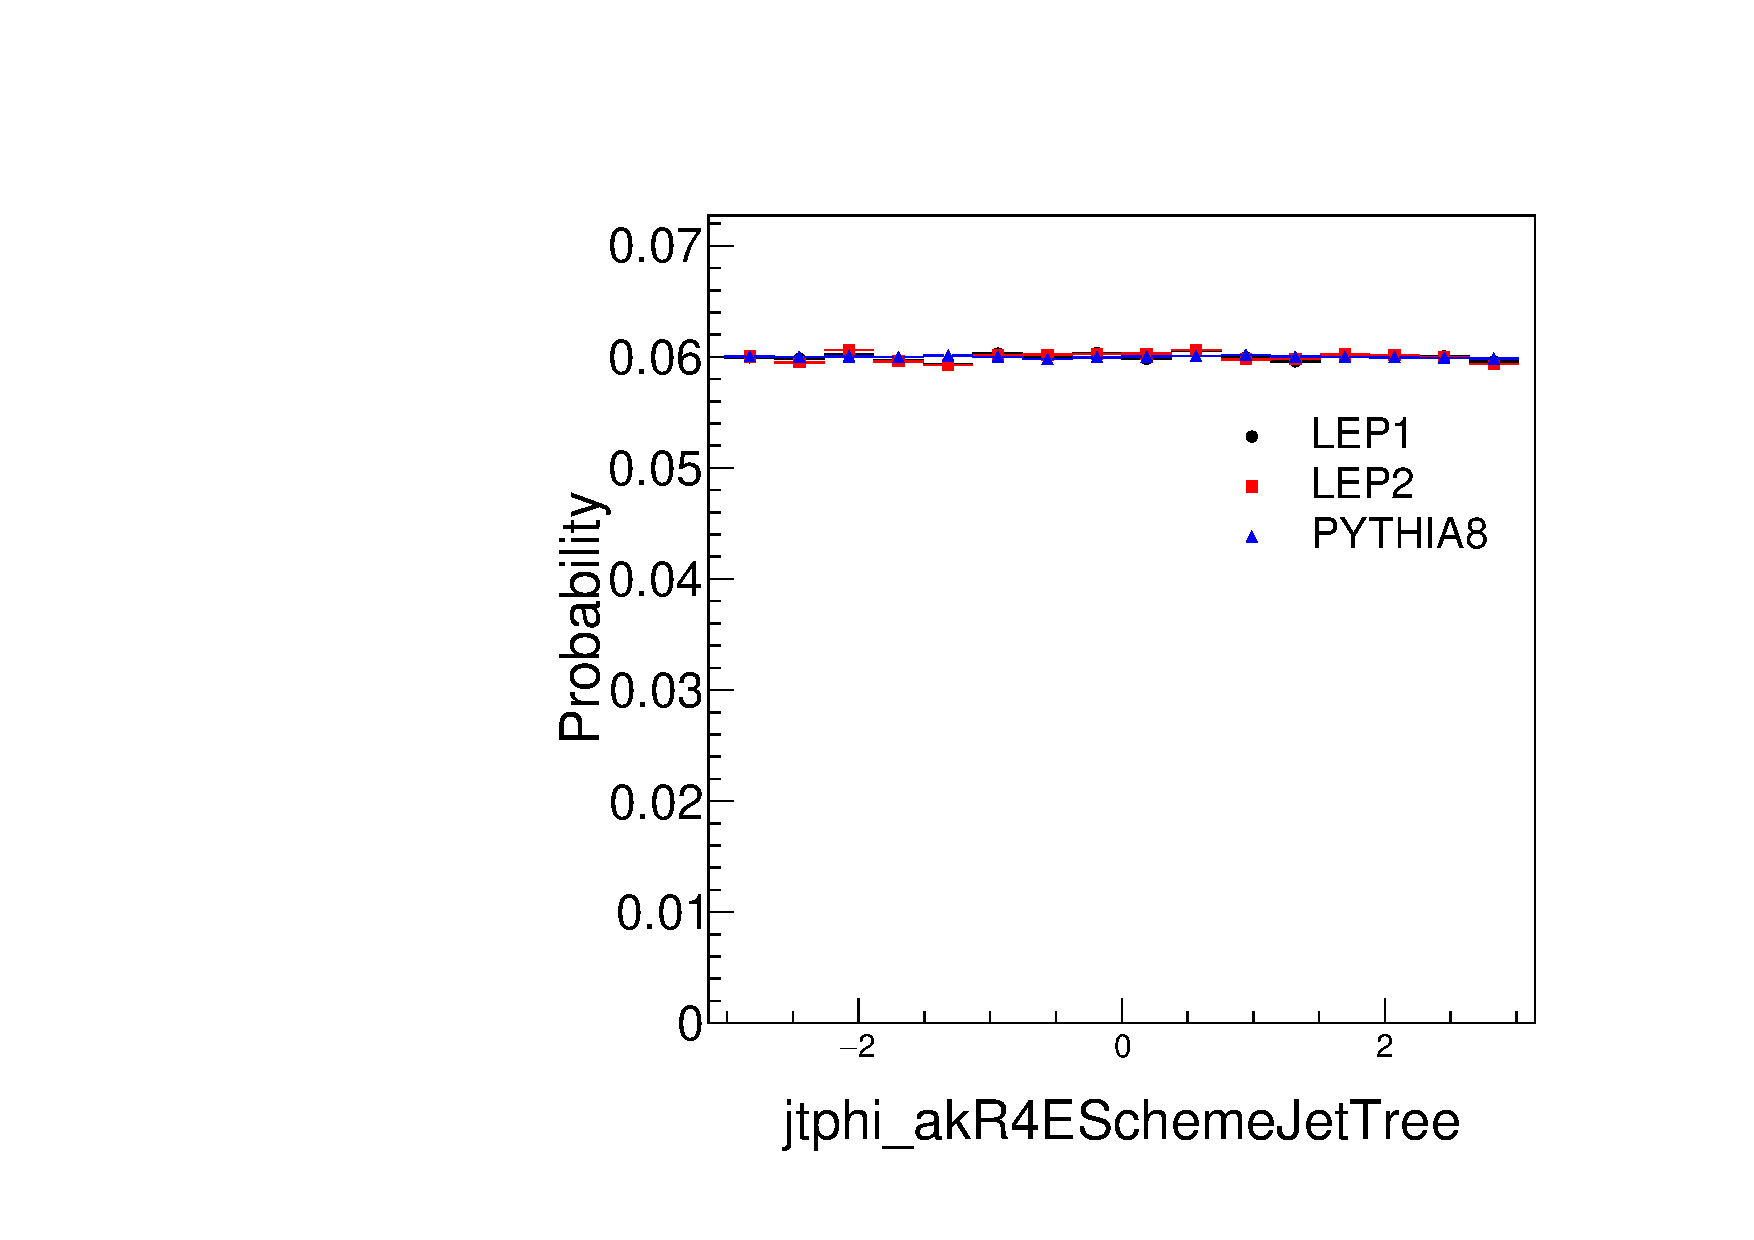
\includegraphics[width=.25\textwidth]{images/DQC/LEP1MC/jtphi_akR4ESchemeJetTree.pdf}}\hfill
\subfloat{\label{sfig:b}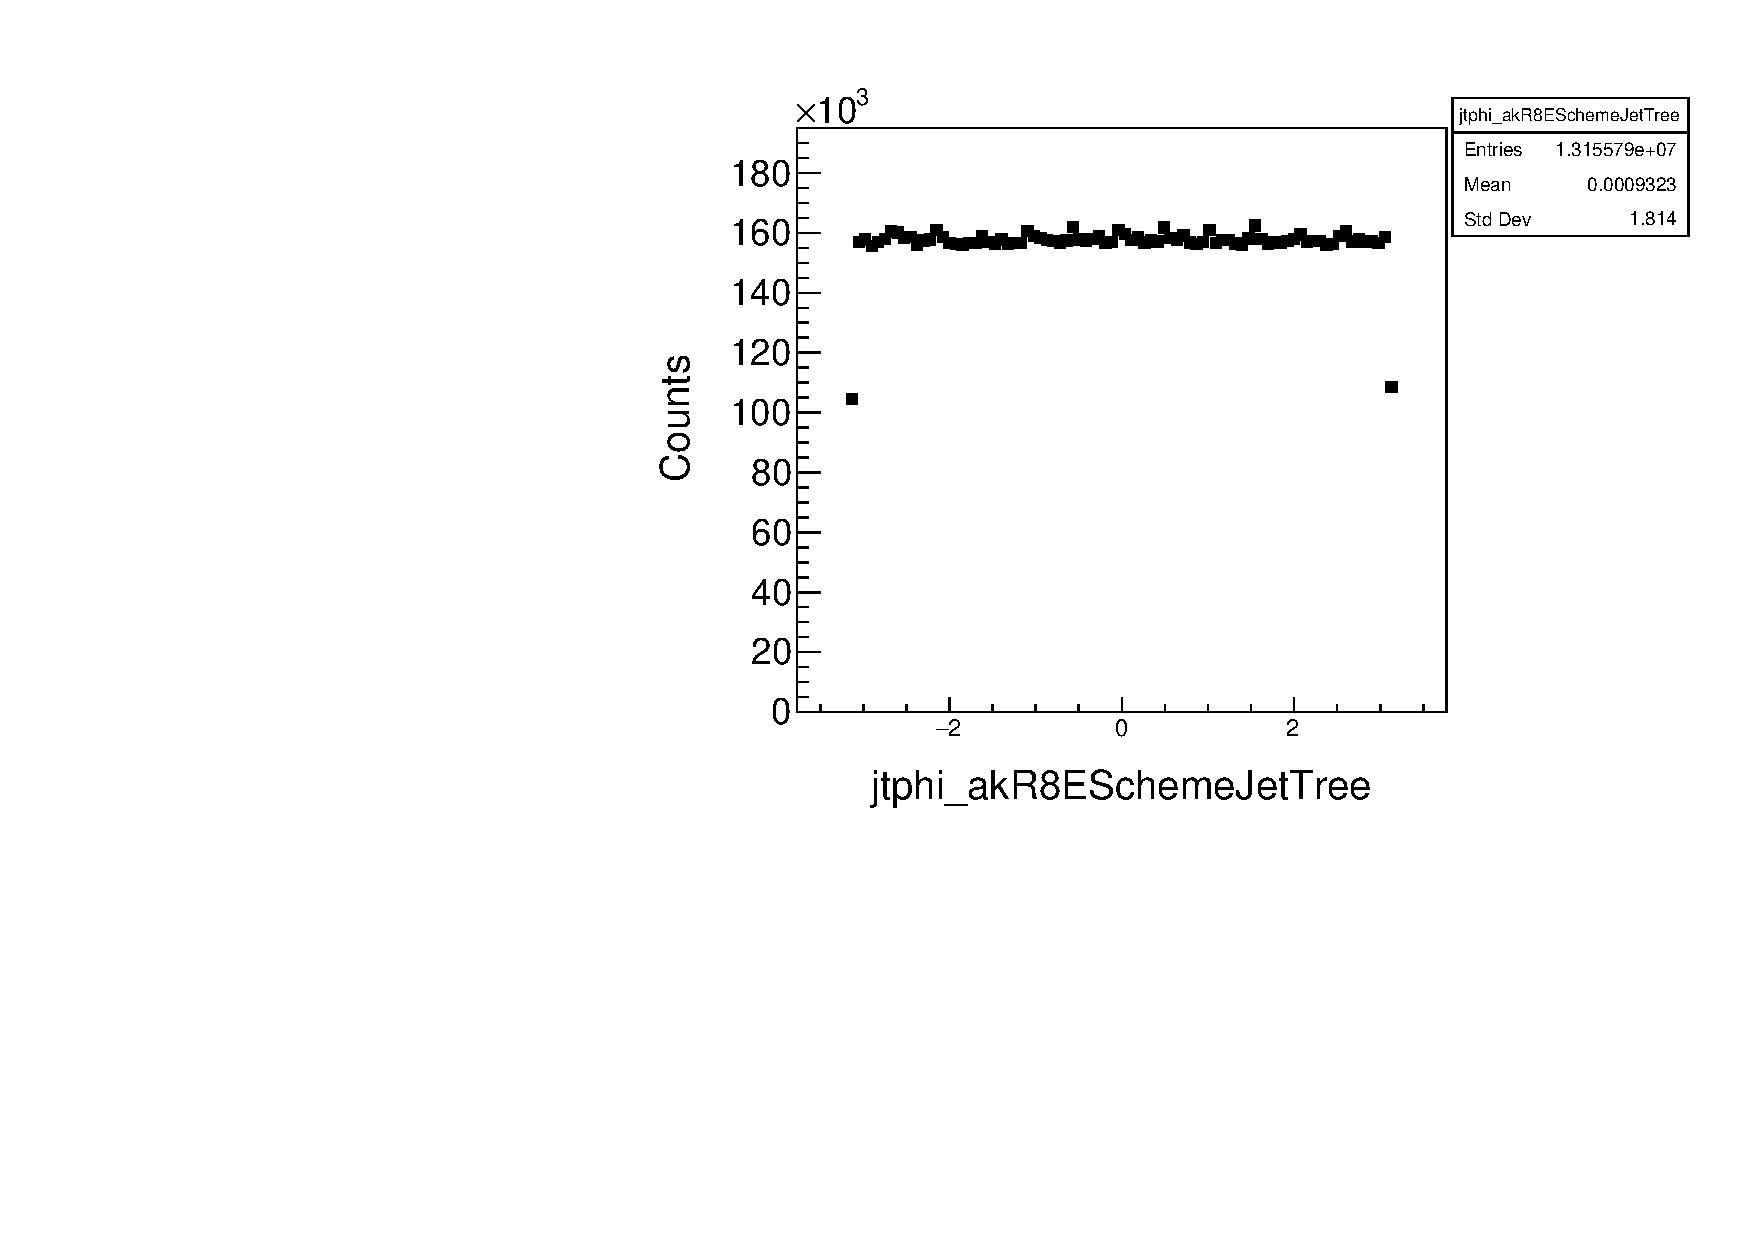
\includegraphics[width=.25\textwidth]{images/DQC/LEP1MC/jtphi_akR8ESchemeJetTree.pdf}}\hfill
\subfloat{\label{sfig:c}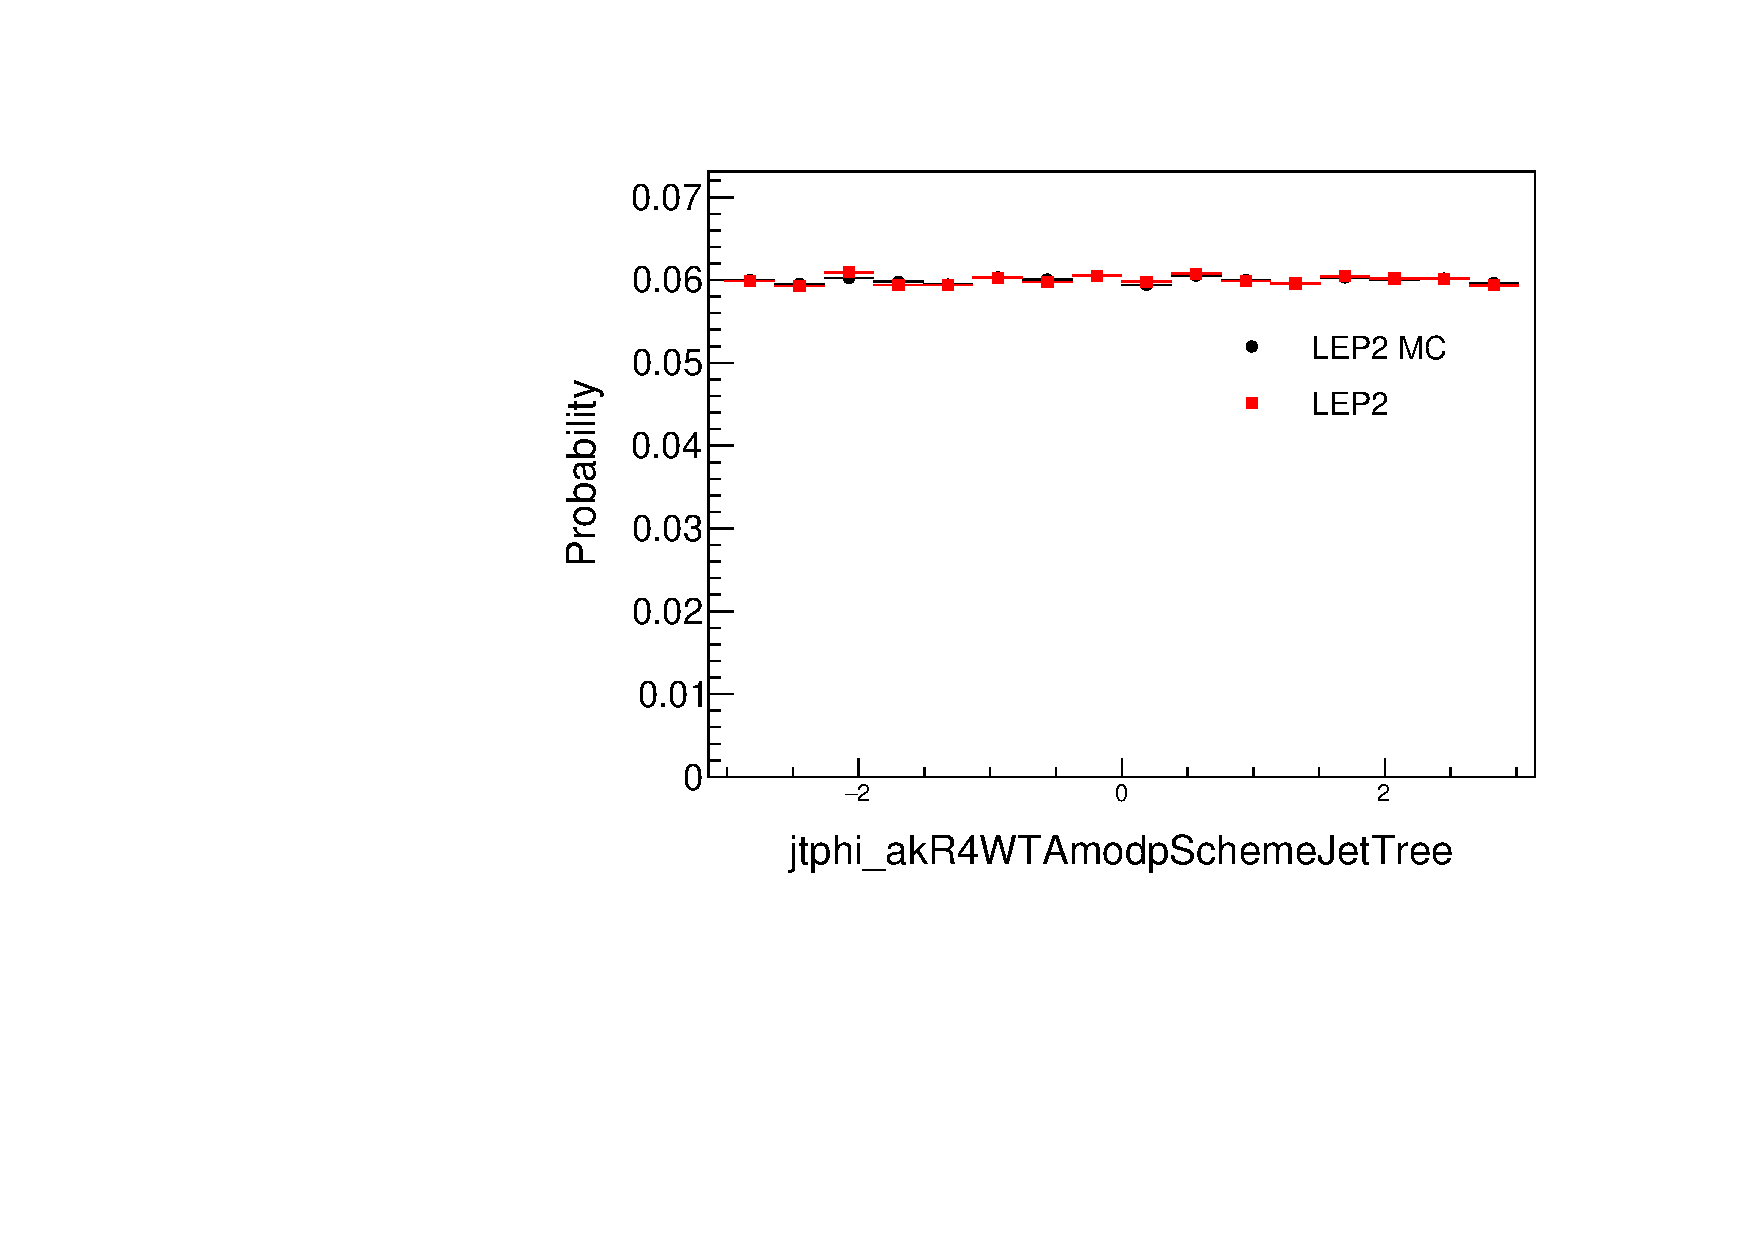
\includegraphics[width=.25\textwidth]{images/DQC/LEP1MC/jtphi_akR4WTAmodpSchemeJetTree.pdf}}\hfill
\subfloat{\label{sfig:d}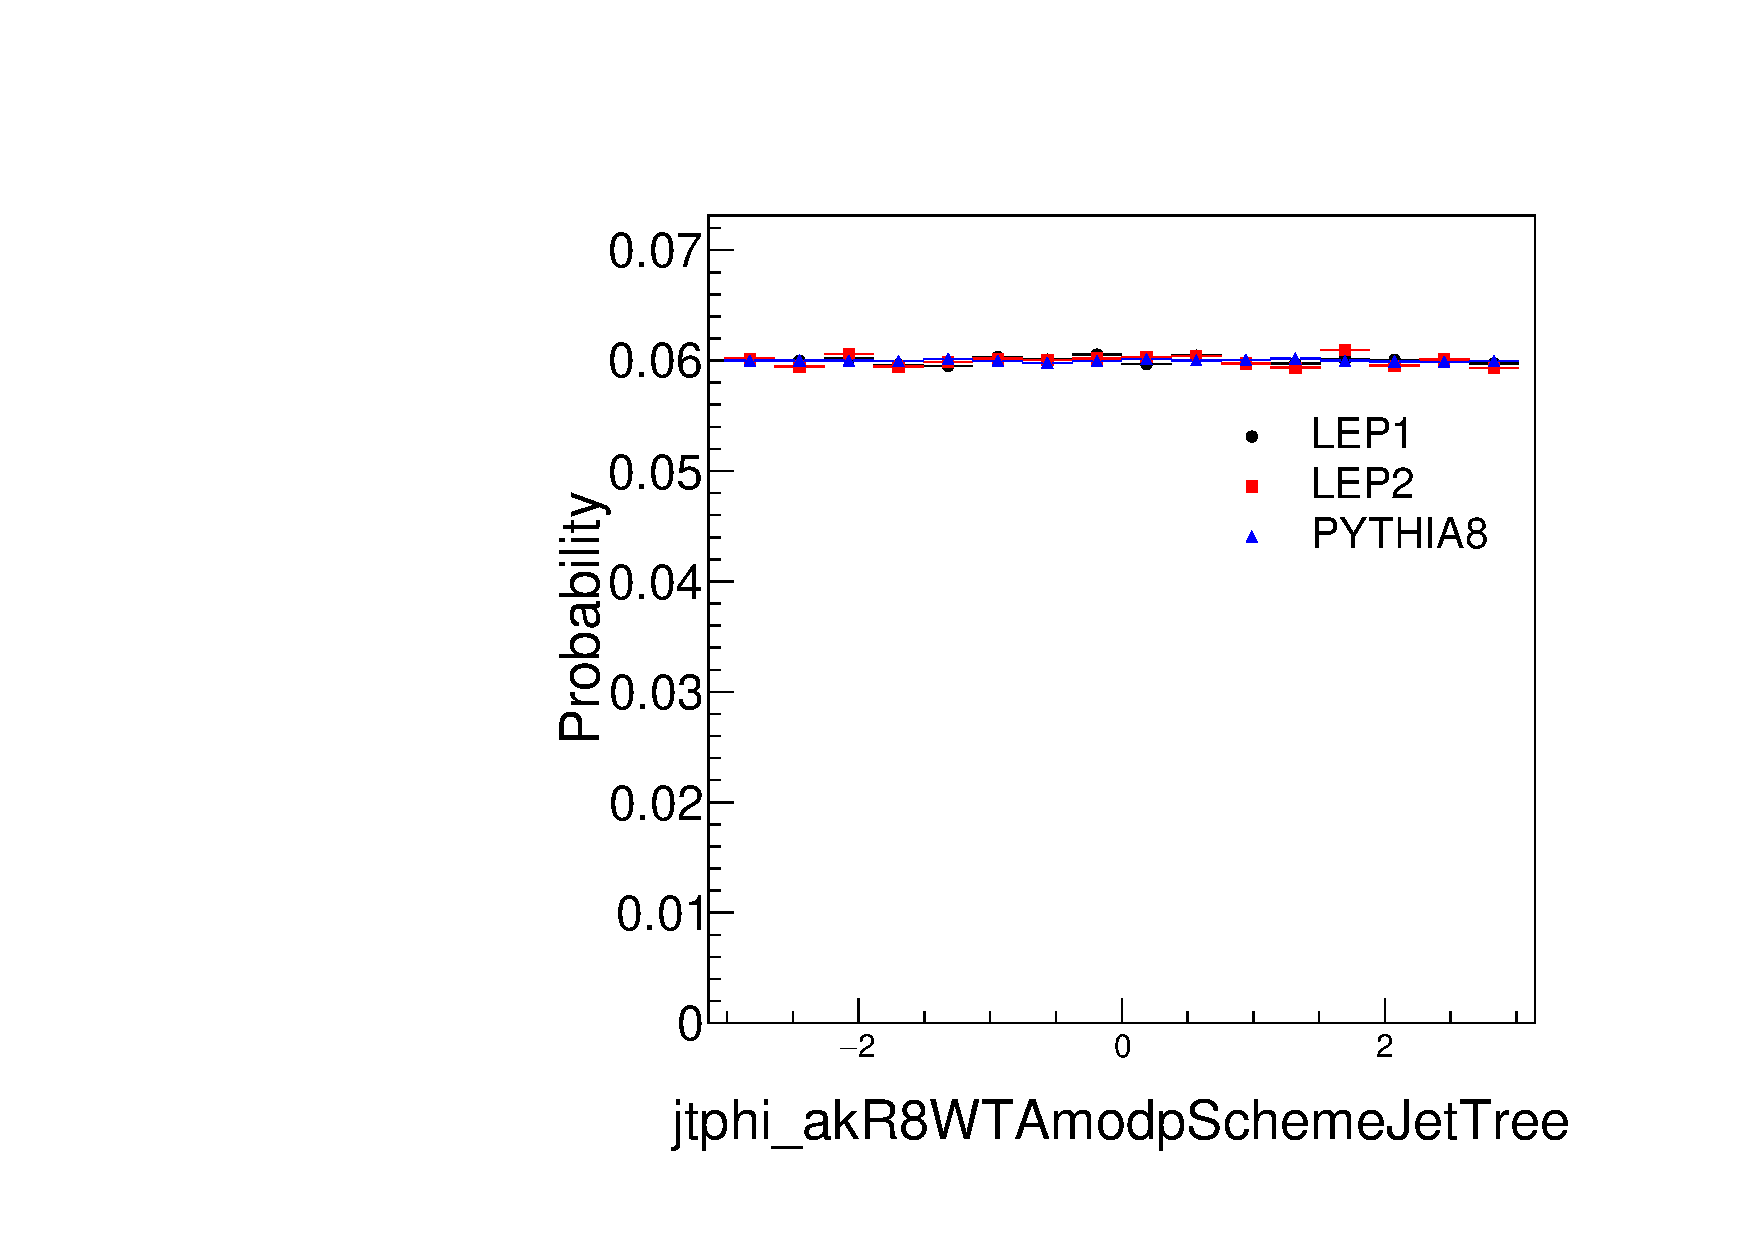
\includegraphics[width=.25\textwidth]{images/DQC/LEP1MC/jtphi_akR8WTAmodpSchemeJetTree.pdf}}\hfill %row end
\subfloat{\label{sfig:e}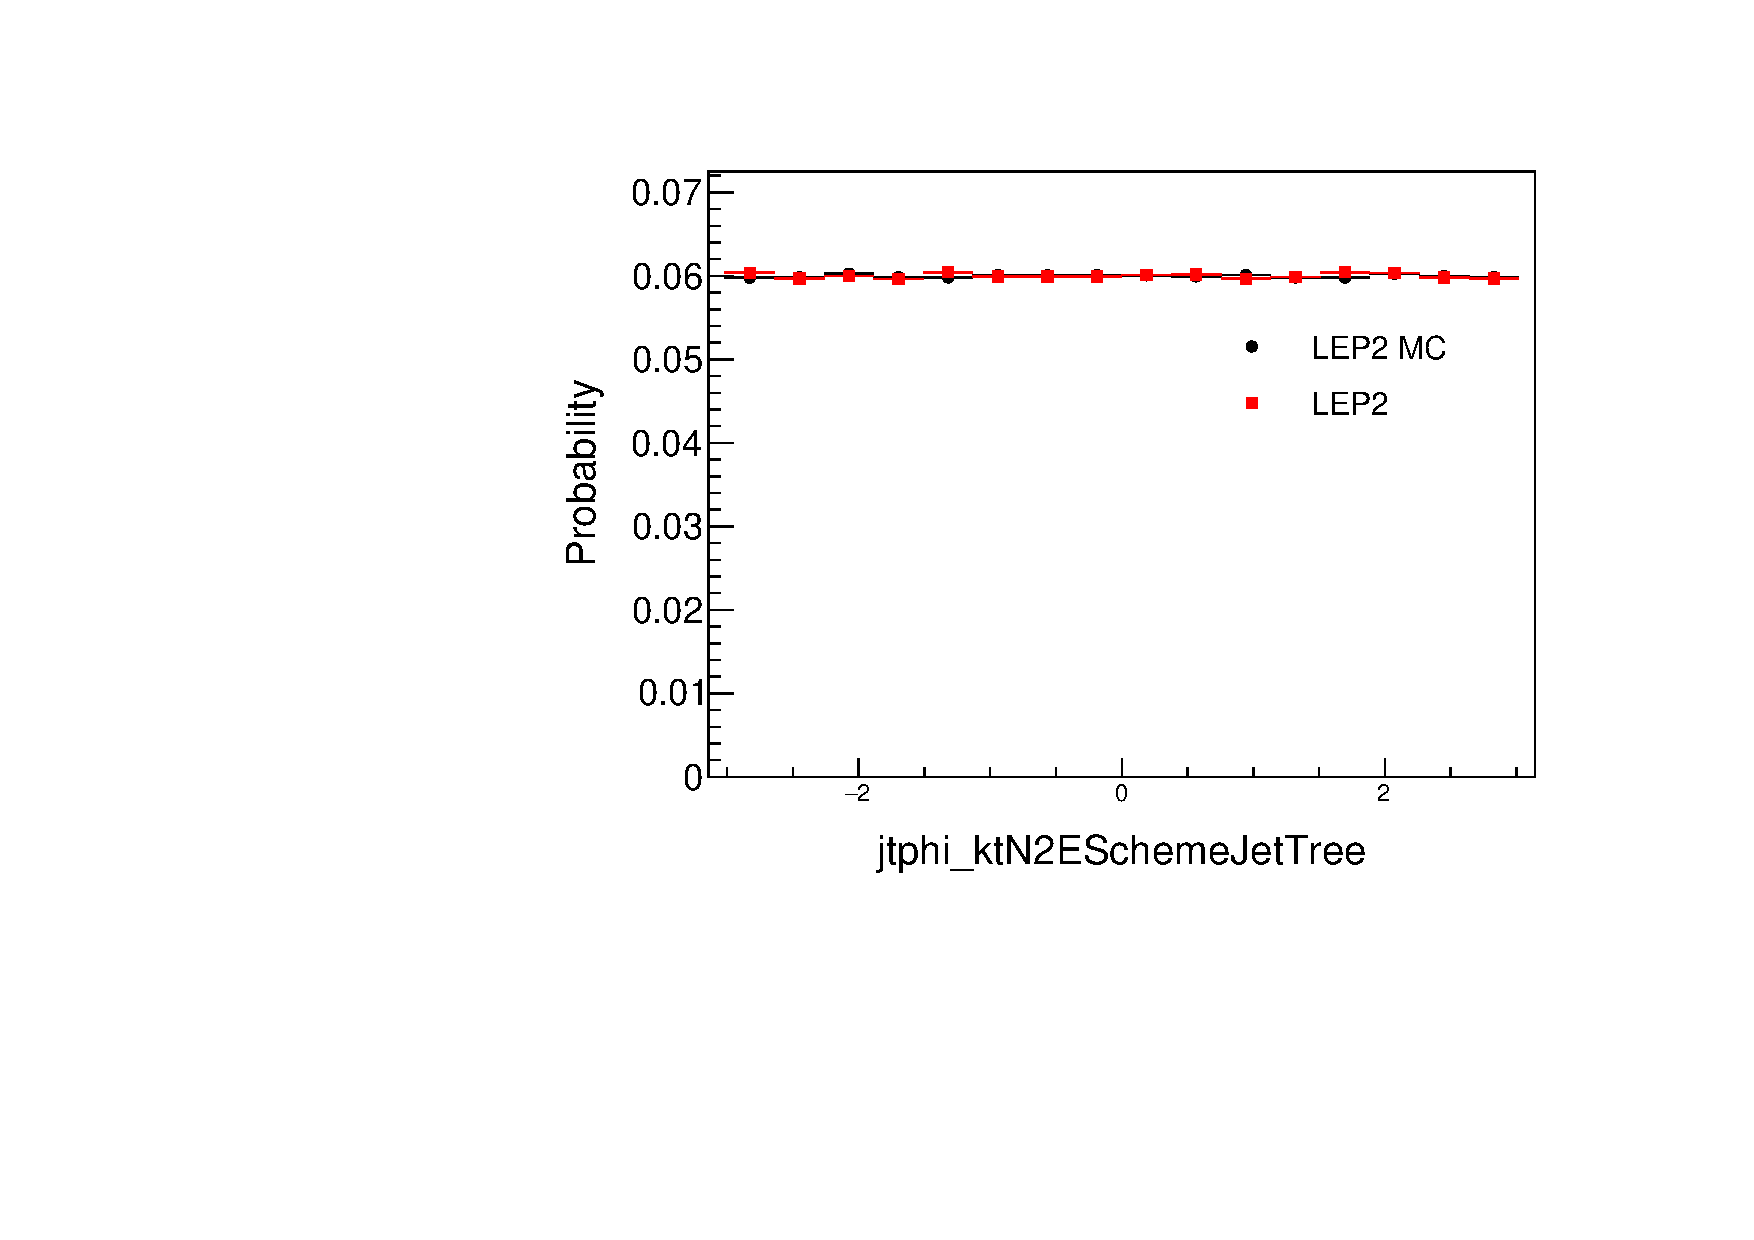
\includegraphics[width=.25\textwidth]{images/DQC/LEP1MC/jtphi_ktN2ESchemeJetTree.pdf}}\hfill
\subfloat{\label{sfig:f}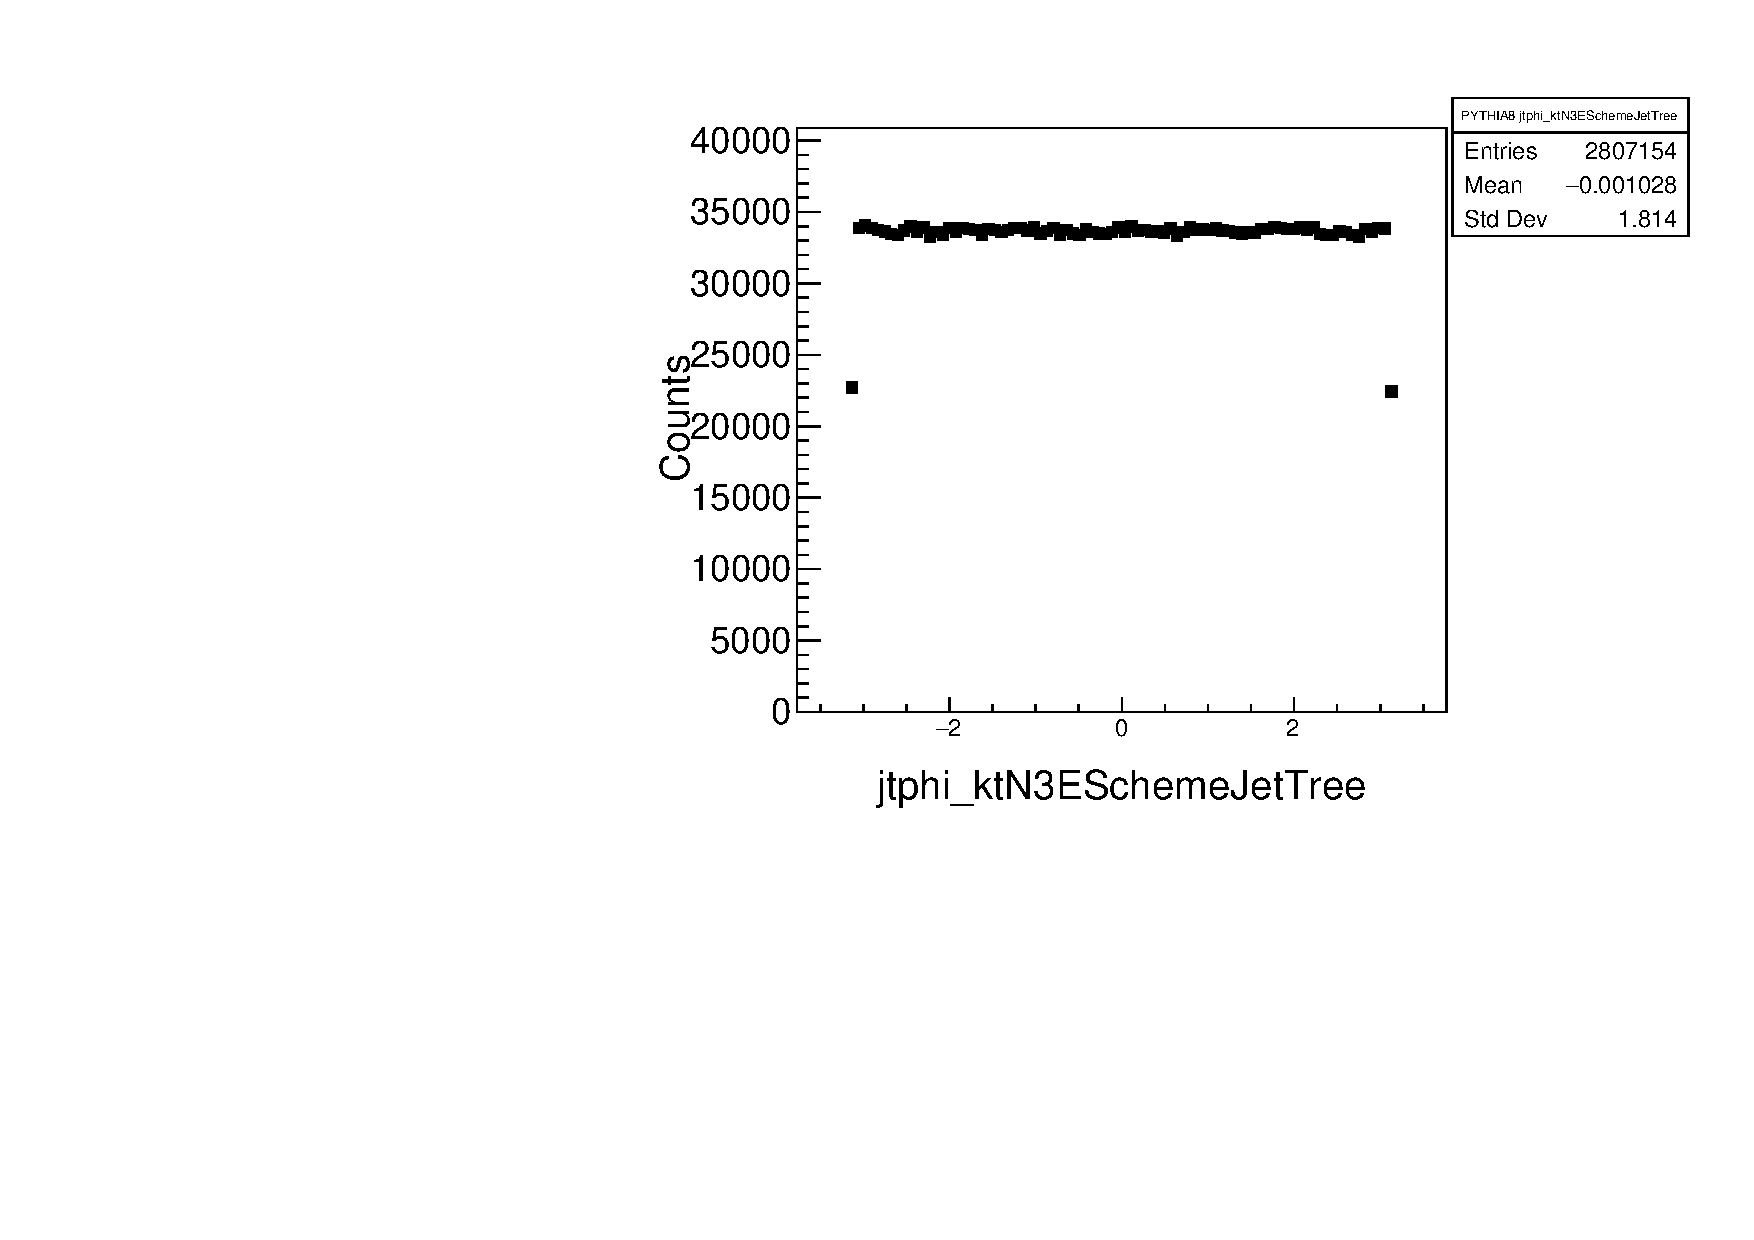
\includegraphics[width=.25\textwidth]{images/DQC/LEP1MC/jtphi_ktN3ESchemeJetTree.pdf}}\hfill
\subfloat{\label{sfig:g}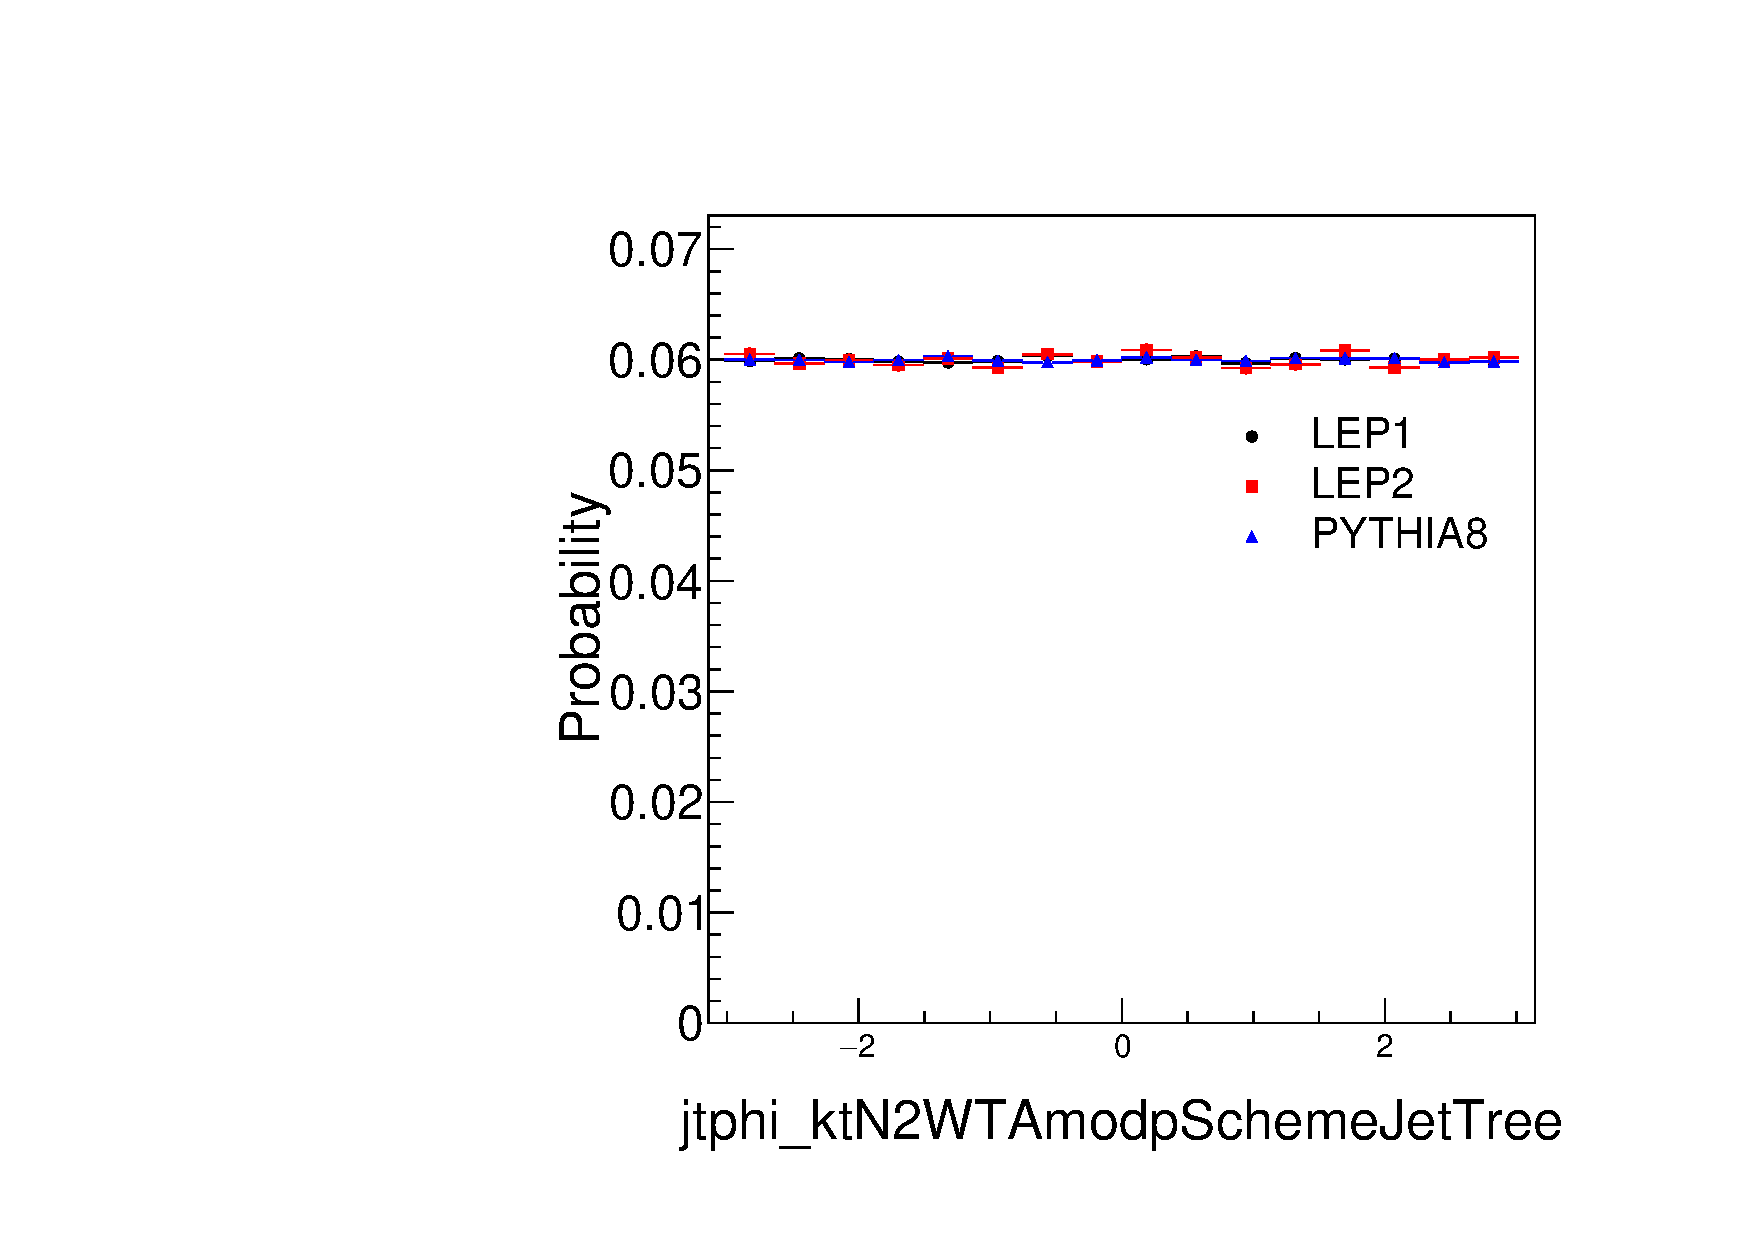
\includegraphics[width=.25\textwidth]{images/DQC/LEP1MC/jtphi_ktN2WTAmodpSchemeJetTree.pdf}}\hfill
\subfloat{\label{sfig:h}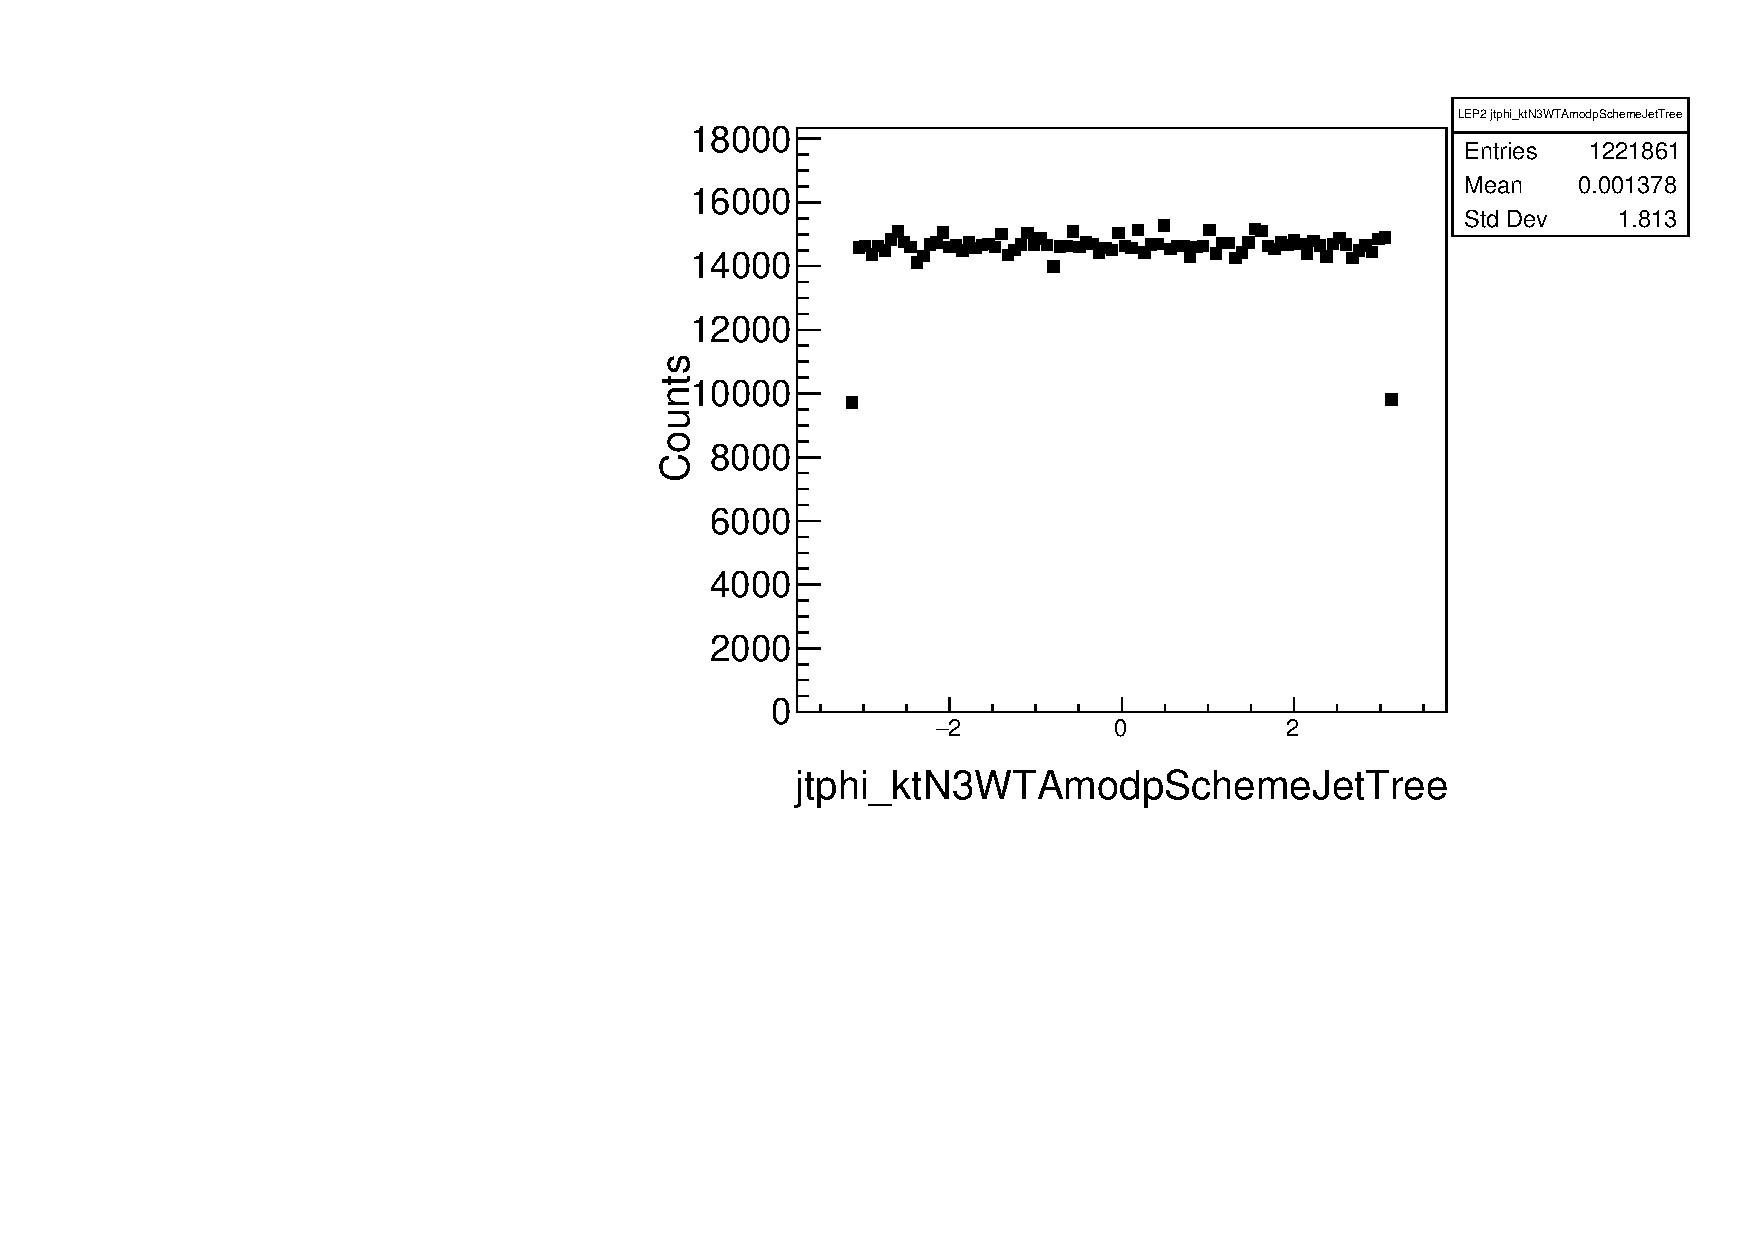
\includegraphics[width=.25\textwidth]{images/DQC/LEP1MC/jtphi_ktN3WTAmodpSchemeJetTree.pdf}}\hfill
\caption{LEP1 vs LEP1 MC Jet $\phi$ distributions. Top row: anti-$k_t$, left to right: $R=0.4$, $E$ scheme; $R=0.8$, $E$ scheme; $R=0.4$, WTA mod p scheme; $R=0.8$, WTA mod p scheme. Bottom row: $k_t$, left to right: $N=2$, $E$ scheme; $N=3$, $E$ scheme; $N=2$, WTA mod p scheme; $N=3$; WTA mod p scheme.}  
\end{figure}

\begin{figure}[H]
\centering
\subfloat{\label{sfig:a}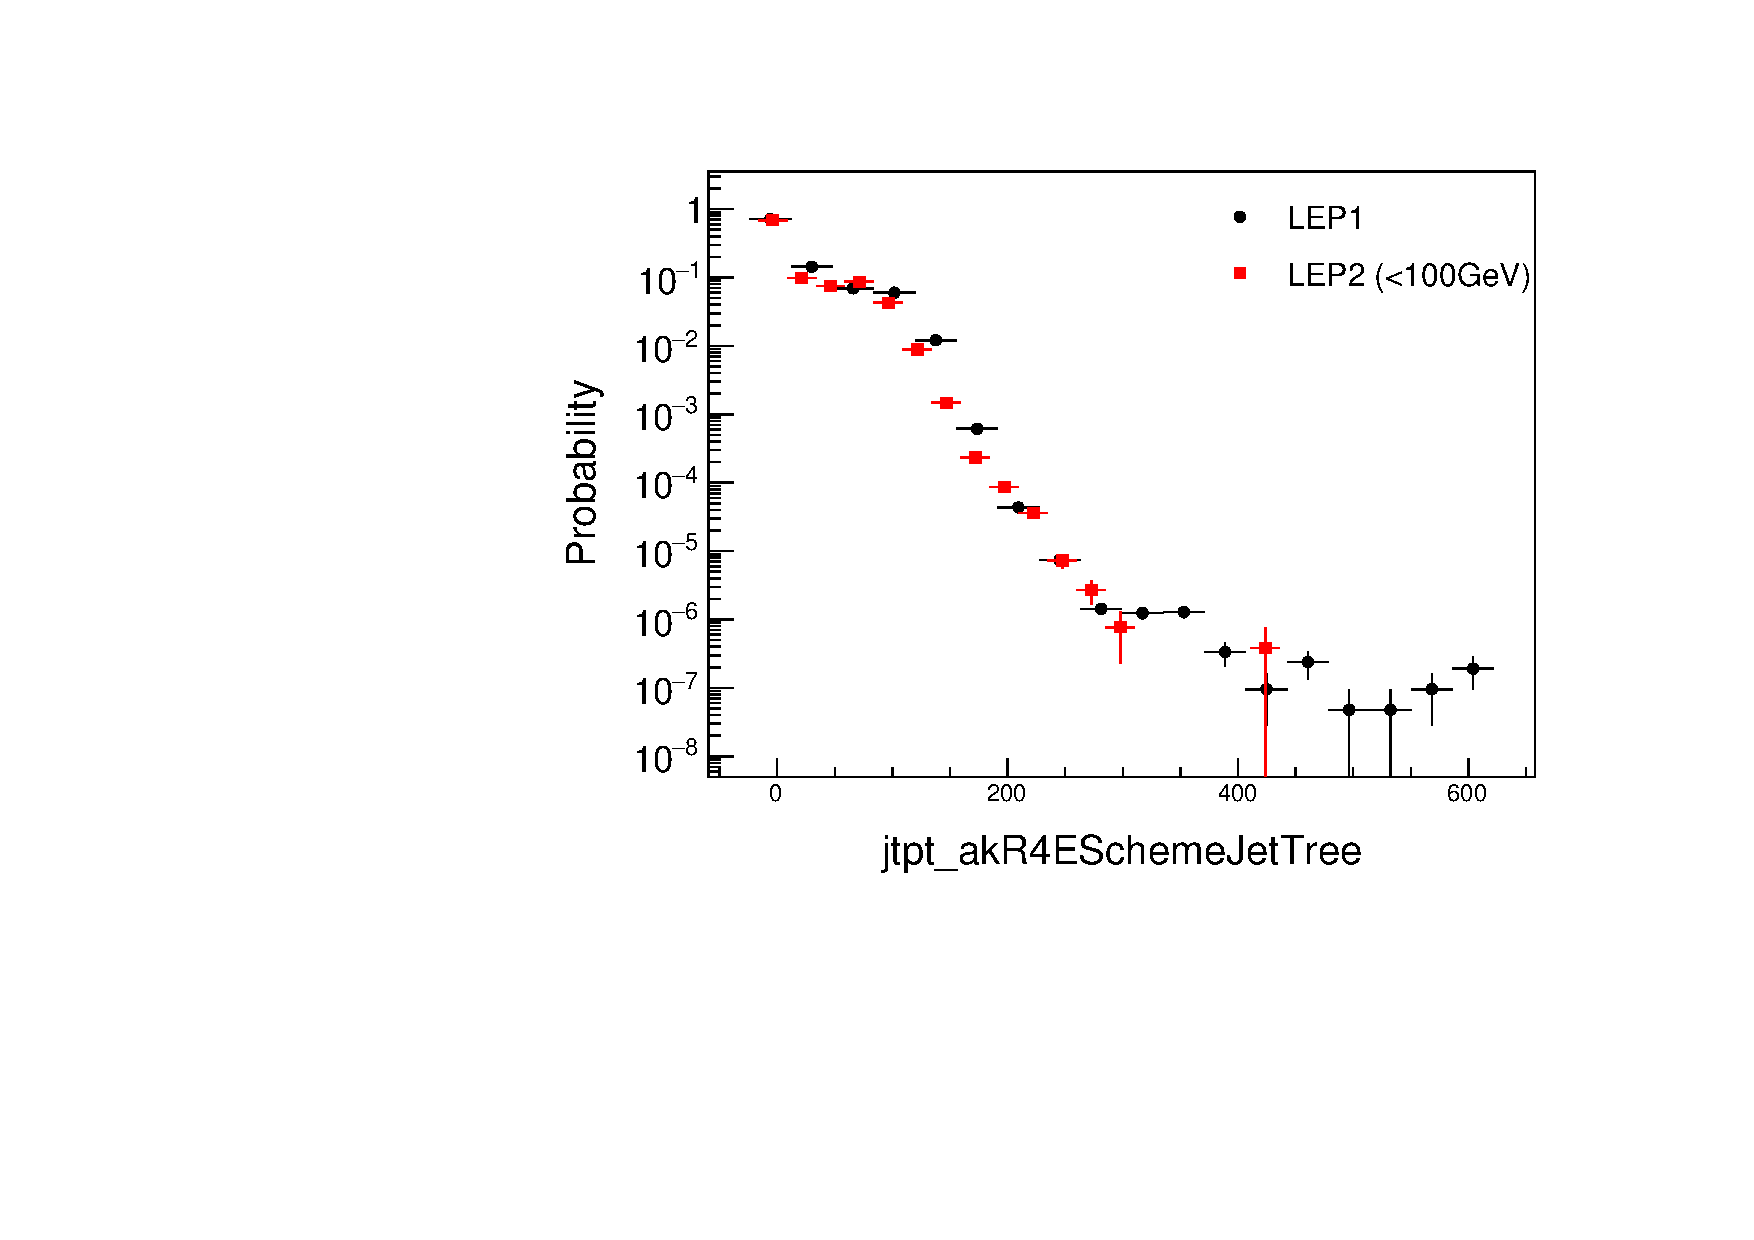
\includegraphics[width=.25\textwidth]{images/DQC/LEP1MC/jtpt_akR4ESchemeJetTree.pdf}}\hfill
\subfloat{\label{sfig:b}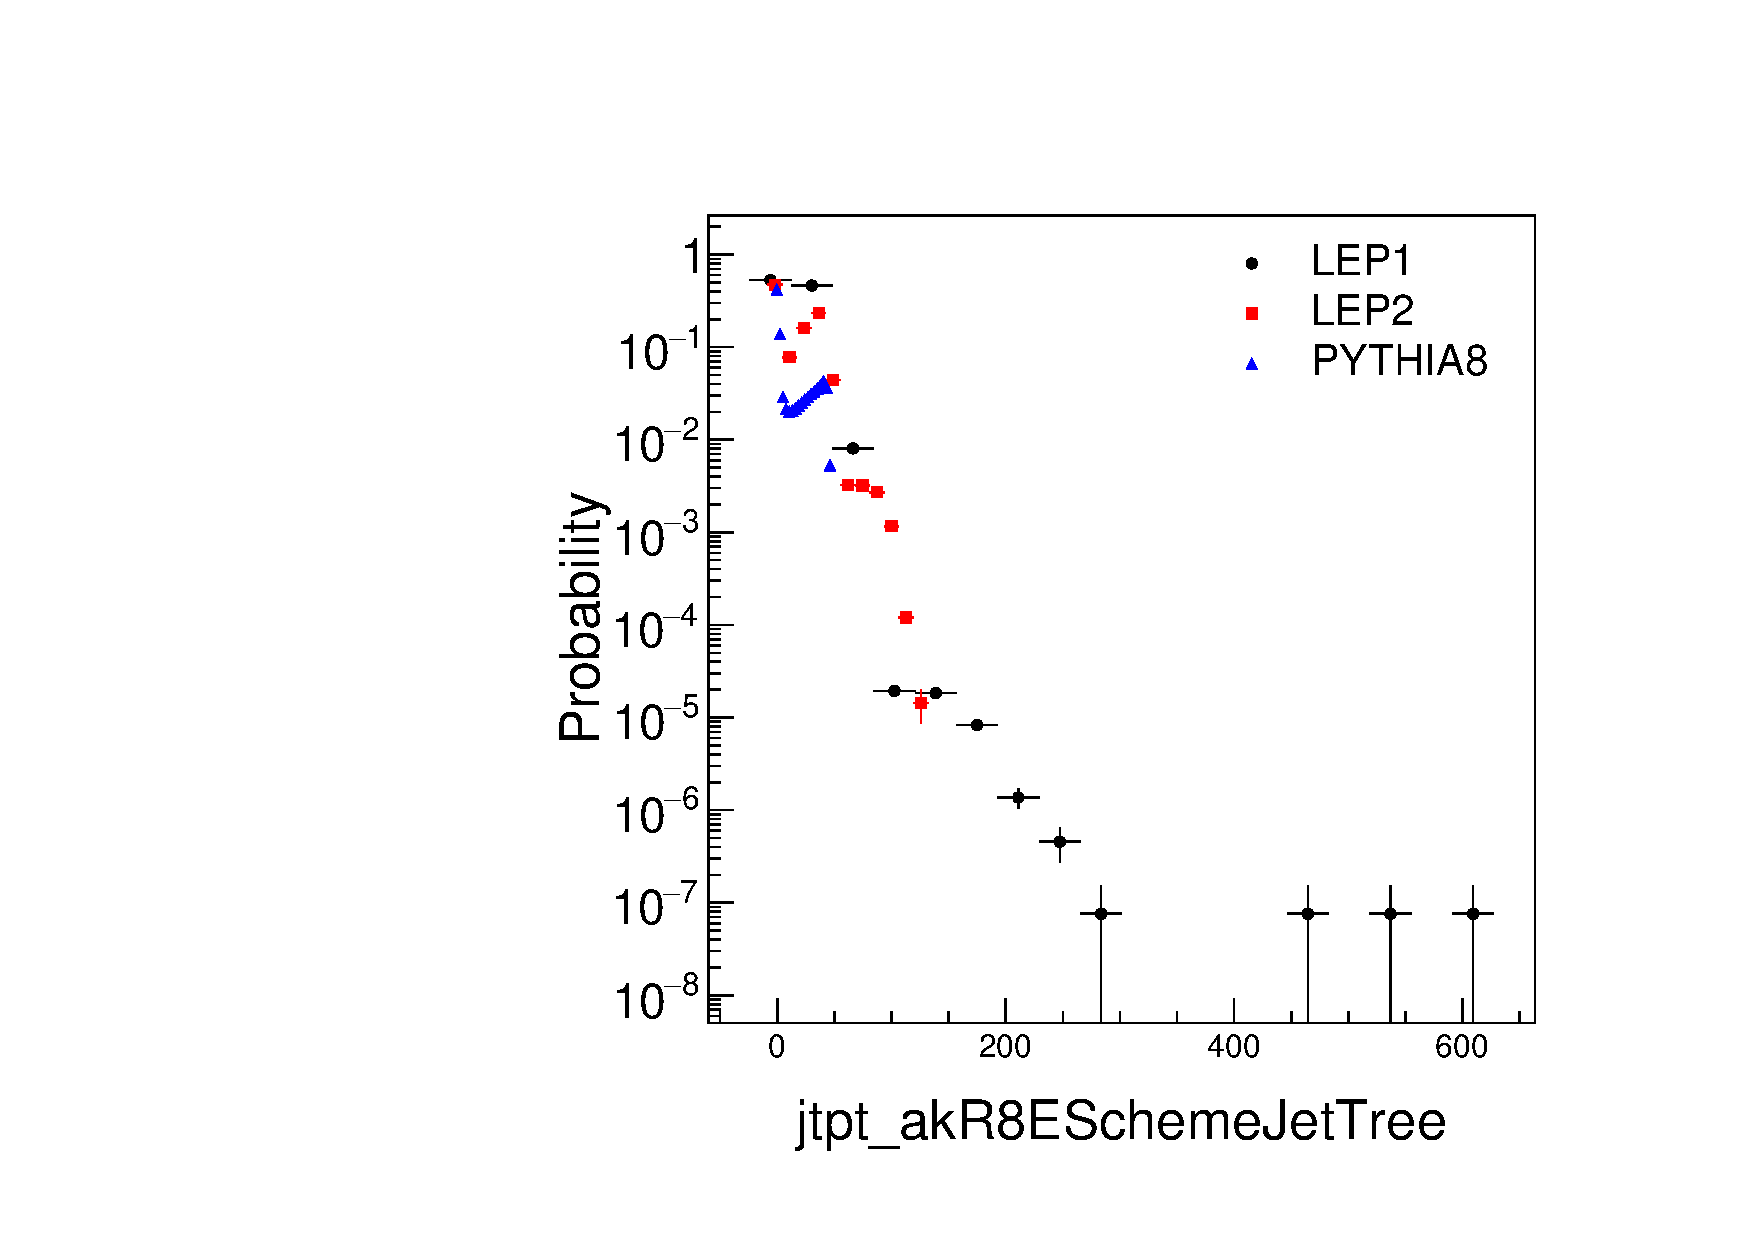
\includegraphics[width=.25\textwidth]{images/DQC/LEP1MC/jtpt_akR8ESchemeJetTree.pdf}}\hfill
\subfloat{\label{sfig:c}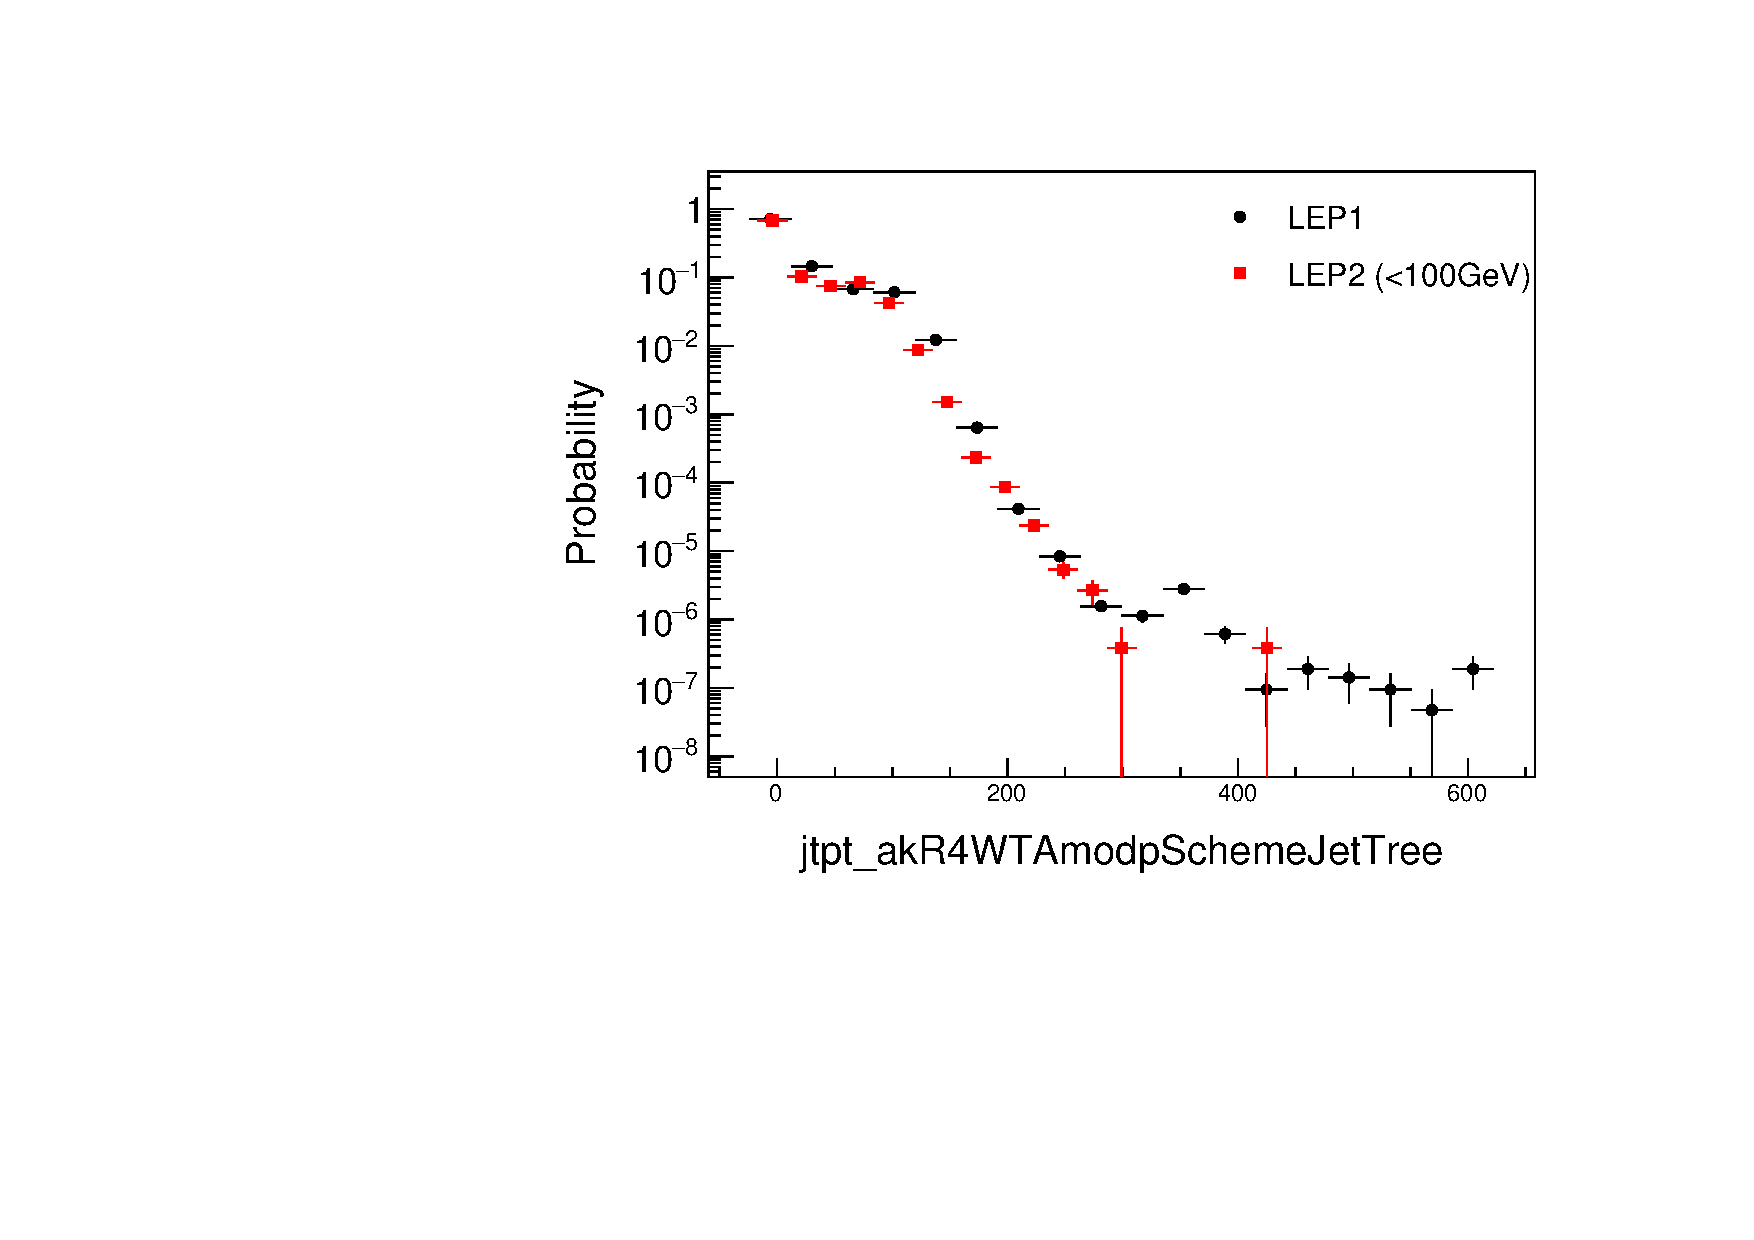
\includegraphics[width=.25\textwidth]{images/DQC/LEP1MC/jtpt_akR4WTAmodpSchemeJetTree.pdf}}\hfill
\subfloat{\label{sfig:d}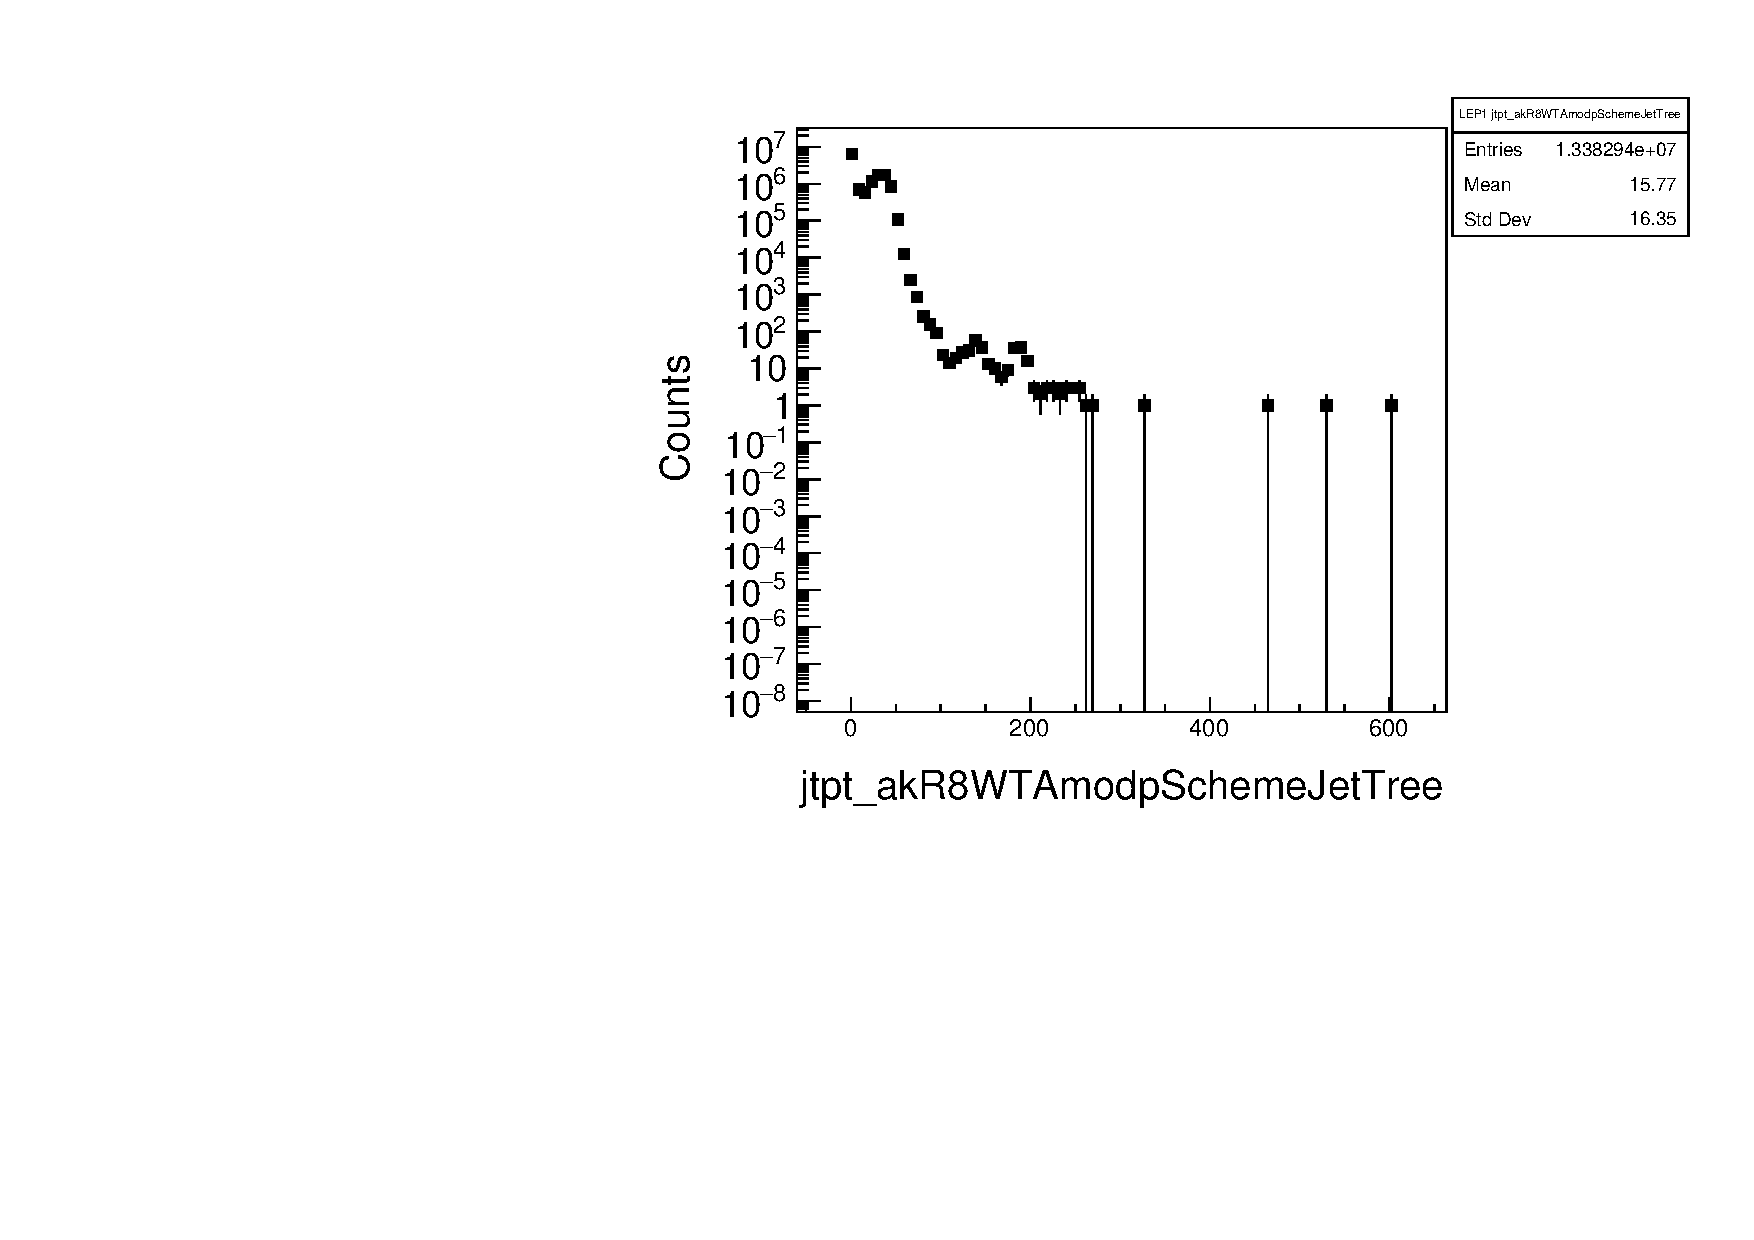
\includegraphics[width=.25\textwidth]{images/DQC/LEP1MC/jtpt_akR8WTAmodpSchemeJetTree.pdf}}\hfill %row end
\subfloat{\label{sfig:e}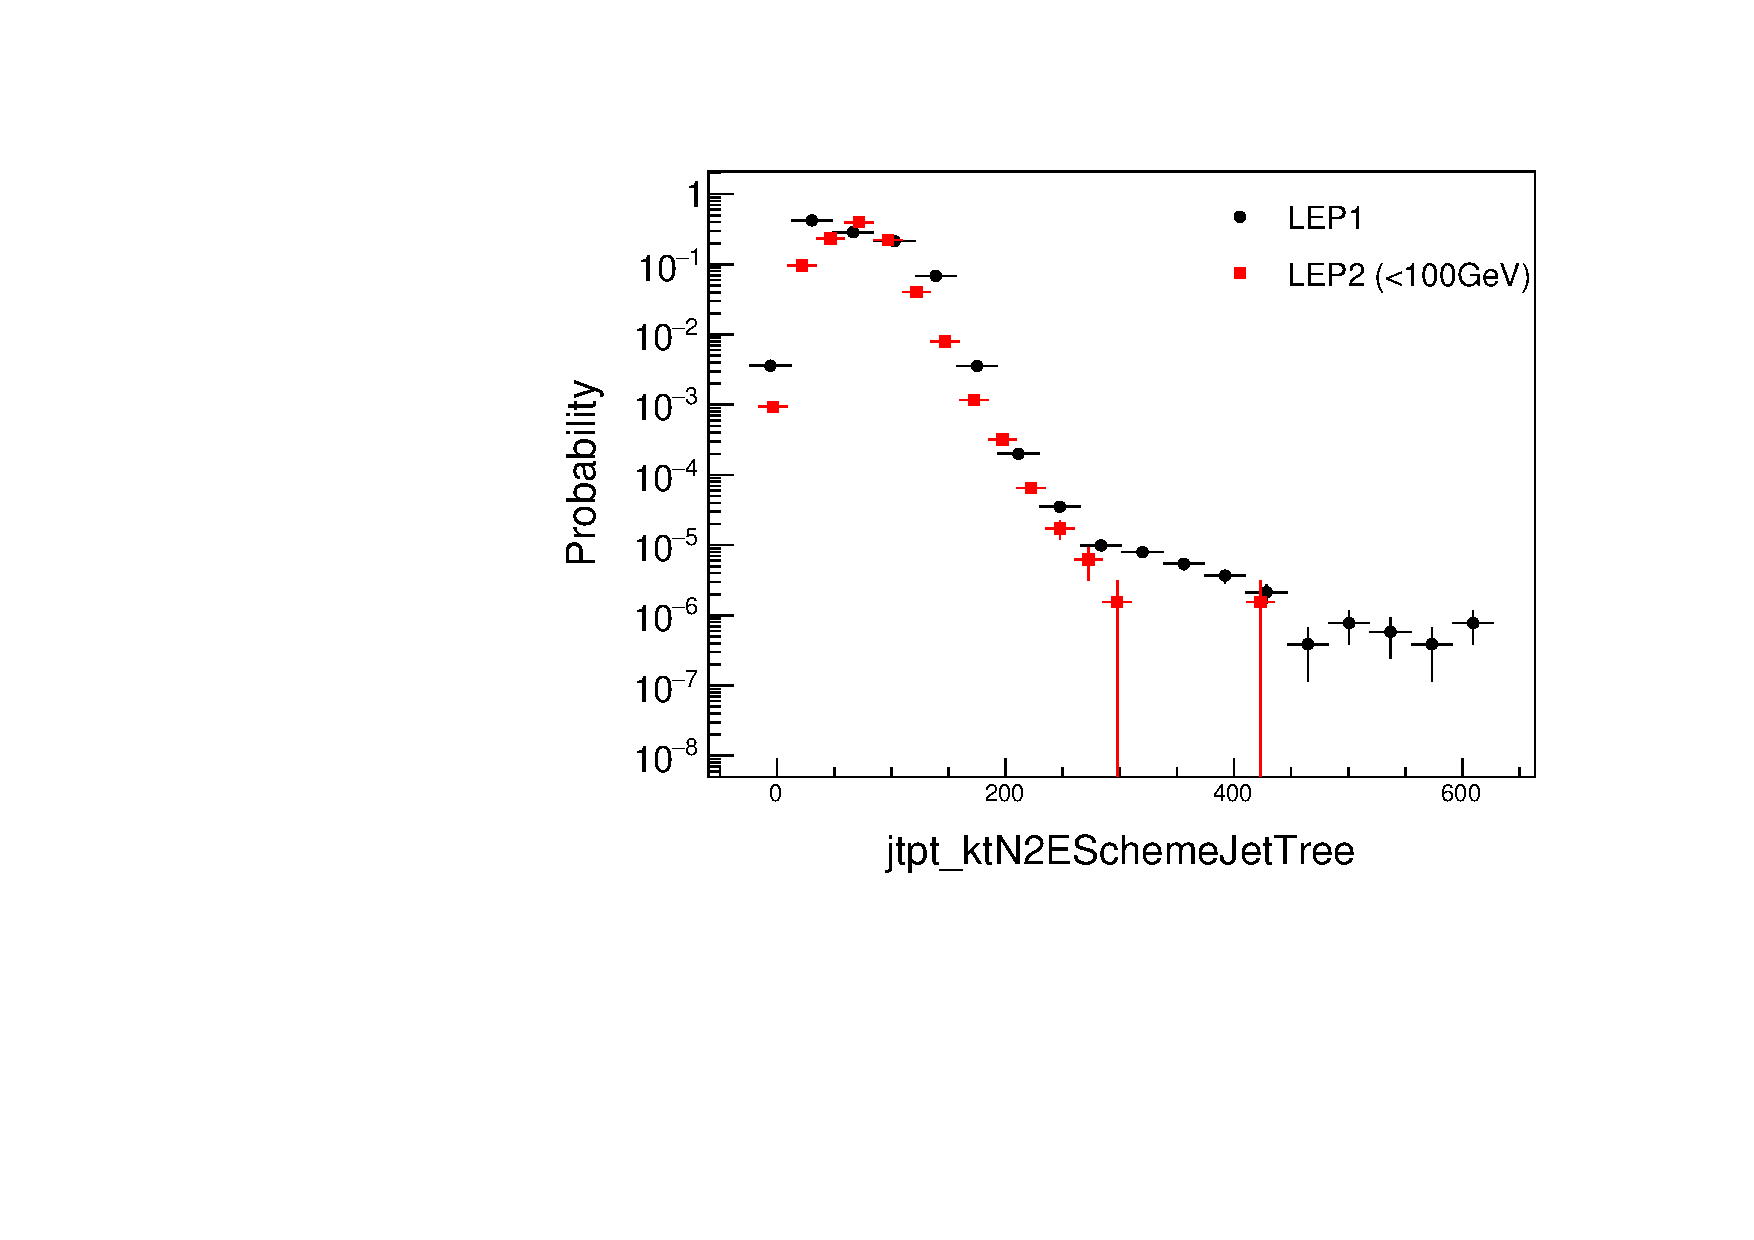
\includegraphics[width=.25\textwidth]{images/DQC/LEP1MC/jtpt_ktN2ESchemeJetTree.pdf}}\hfill
\subfloat{\label{sfig:f}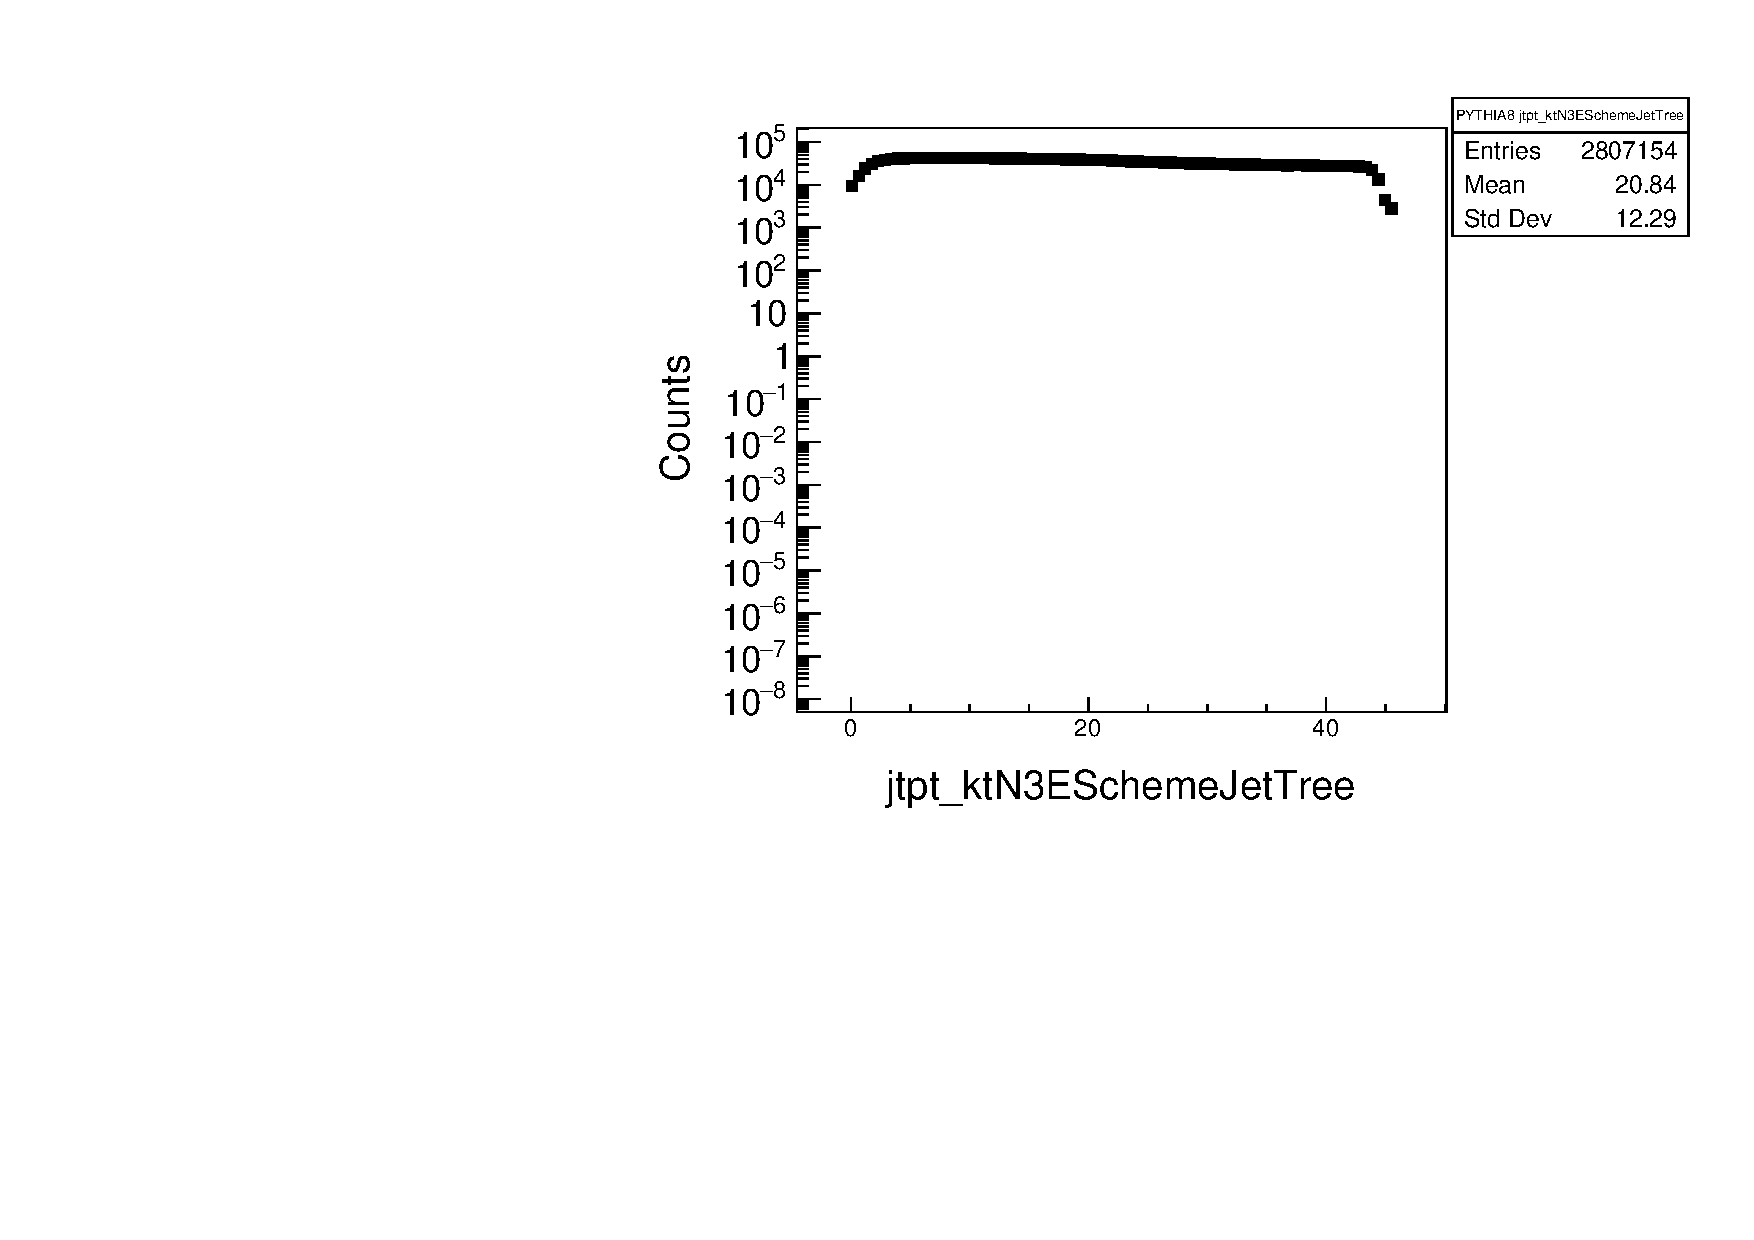
\includegraphics[width=.25\textwidth]{images/DQC/LEP1MC/jtpt_ktN3ESchemeJetTree.pdf}}\hfill
\subfloat{\label{sfig:g}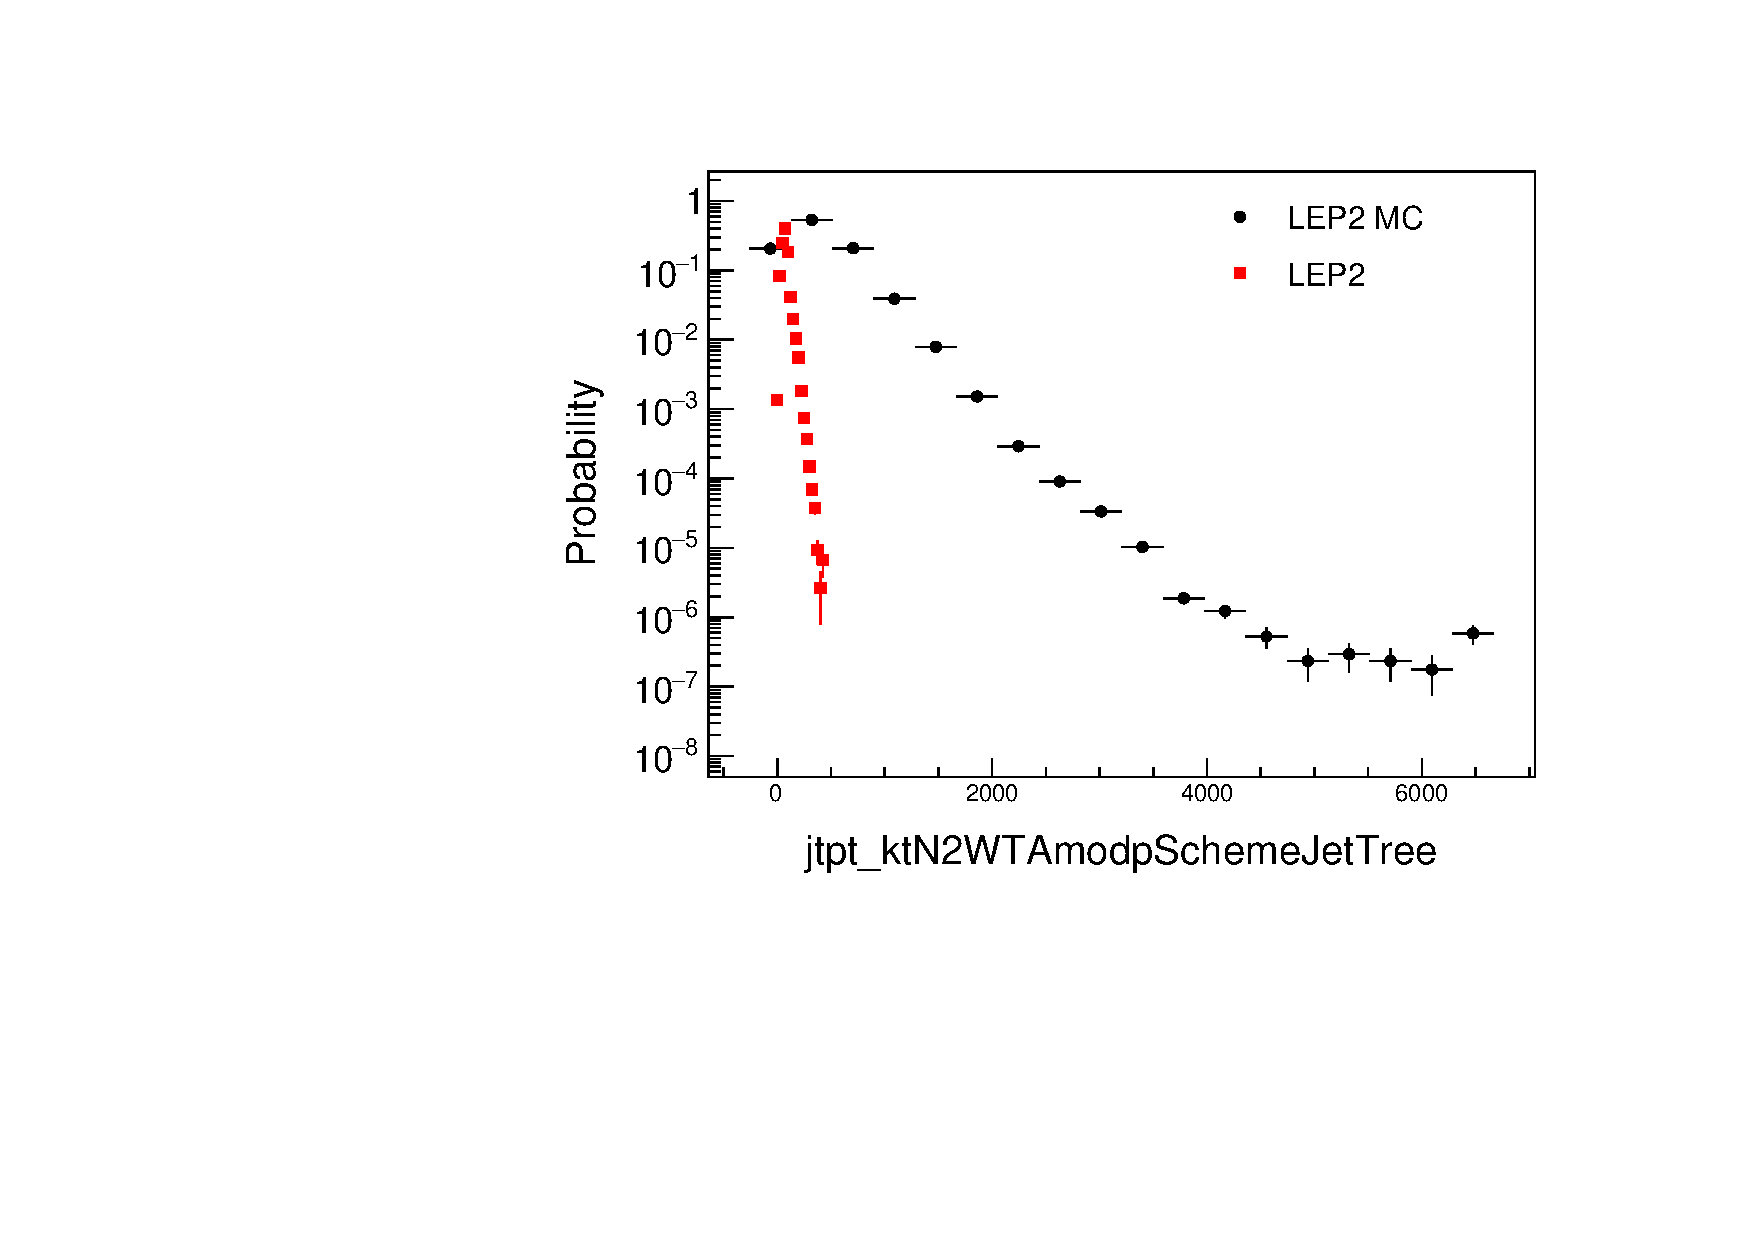
\includegraphics[width=.25\textwidth]{images/DQC/LEP1MC/jtpt_ktN2WTAmodpSchemeJetTree.pdf}}\hfill
\subfloat{\label{sfig:h}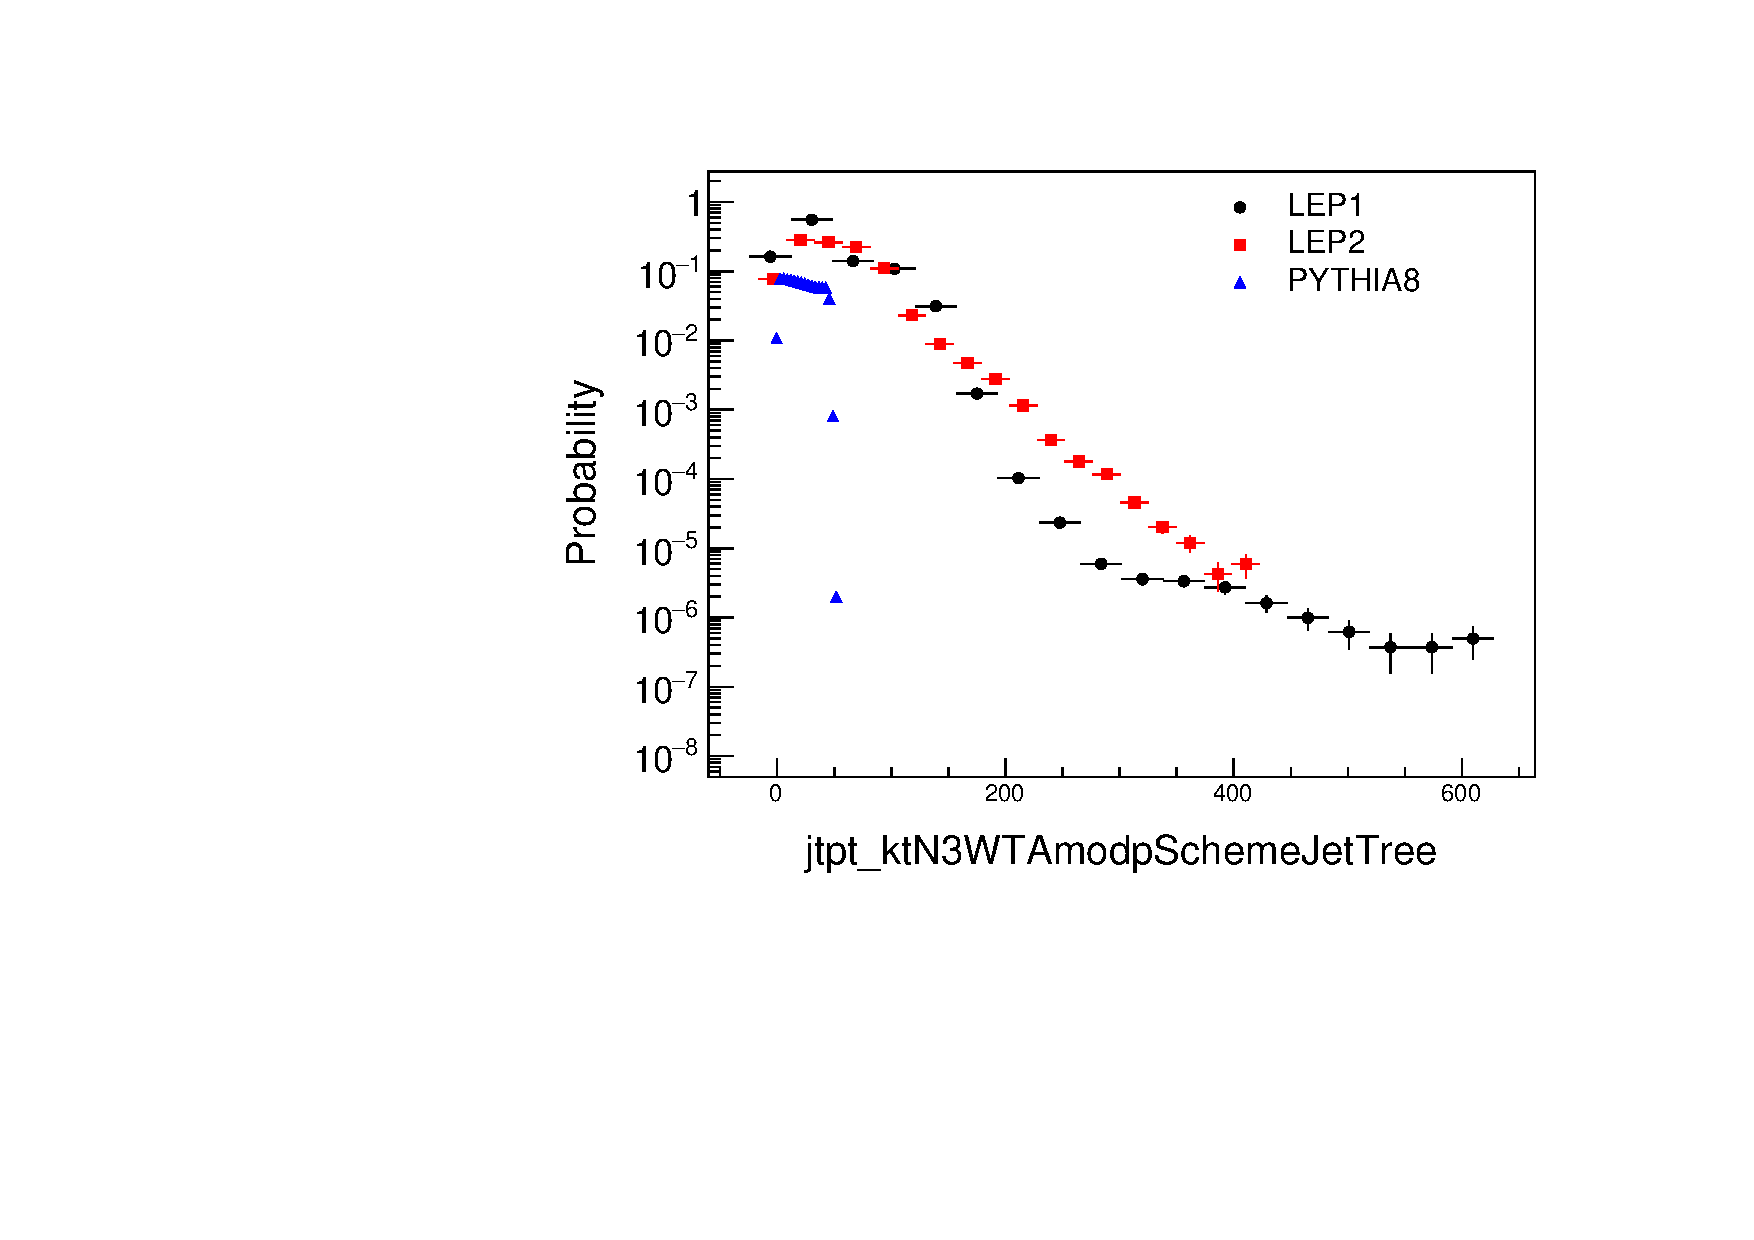
\includegraphics[width=.25\textwidth]{images/DQC/LEP1MC/jtpt_ktN3WTAmodpSchemeJetTree.pdf}}\hfill
\caption{LEP1 vs LEP1 MC Jet $p_t$ distributions. Top row: anti-$k_t$, left to right: $R=0.4$, $E$ scheme; $R=0.8$, $E$ scheme; $R=0.4$, WTA mod p scheme; $R=0.8$, WTA mod p scheme. Bottom row: $k_t$, left to right: $N=2$, $E$ scheme; $N=3$, $E$ scheme; $N=2$, WTA mod p scheme; $N=3$; WTA mod p scheme.}  
\end{figure}

\begin{figure}[H]
\centering
\subfloat{\label{sfig:a}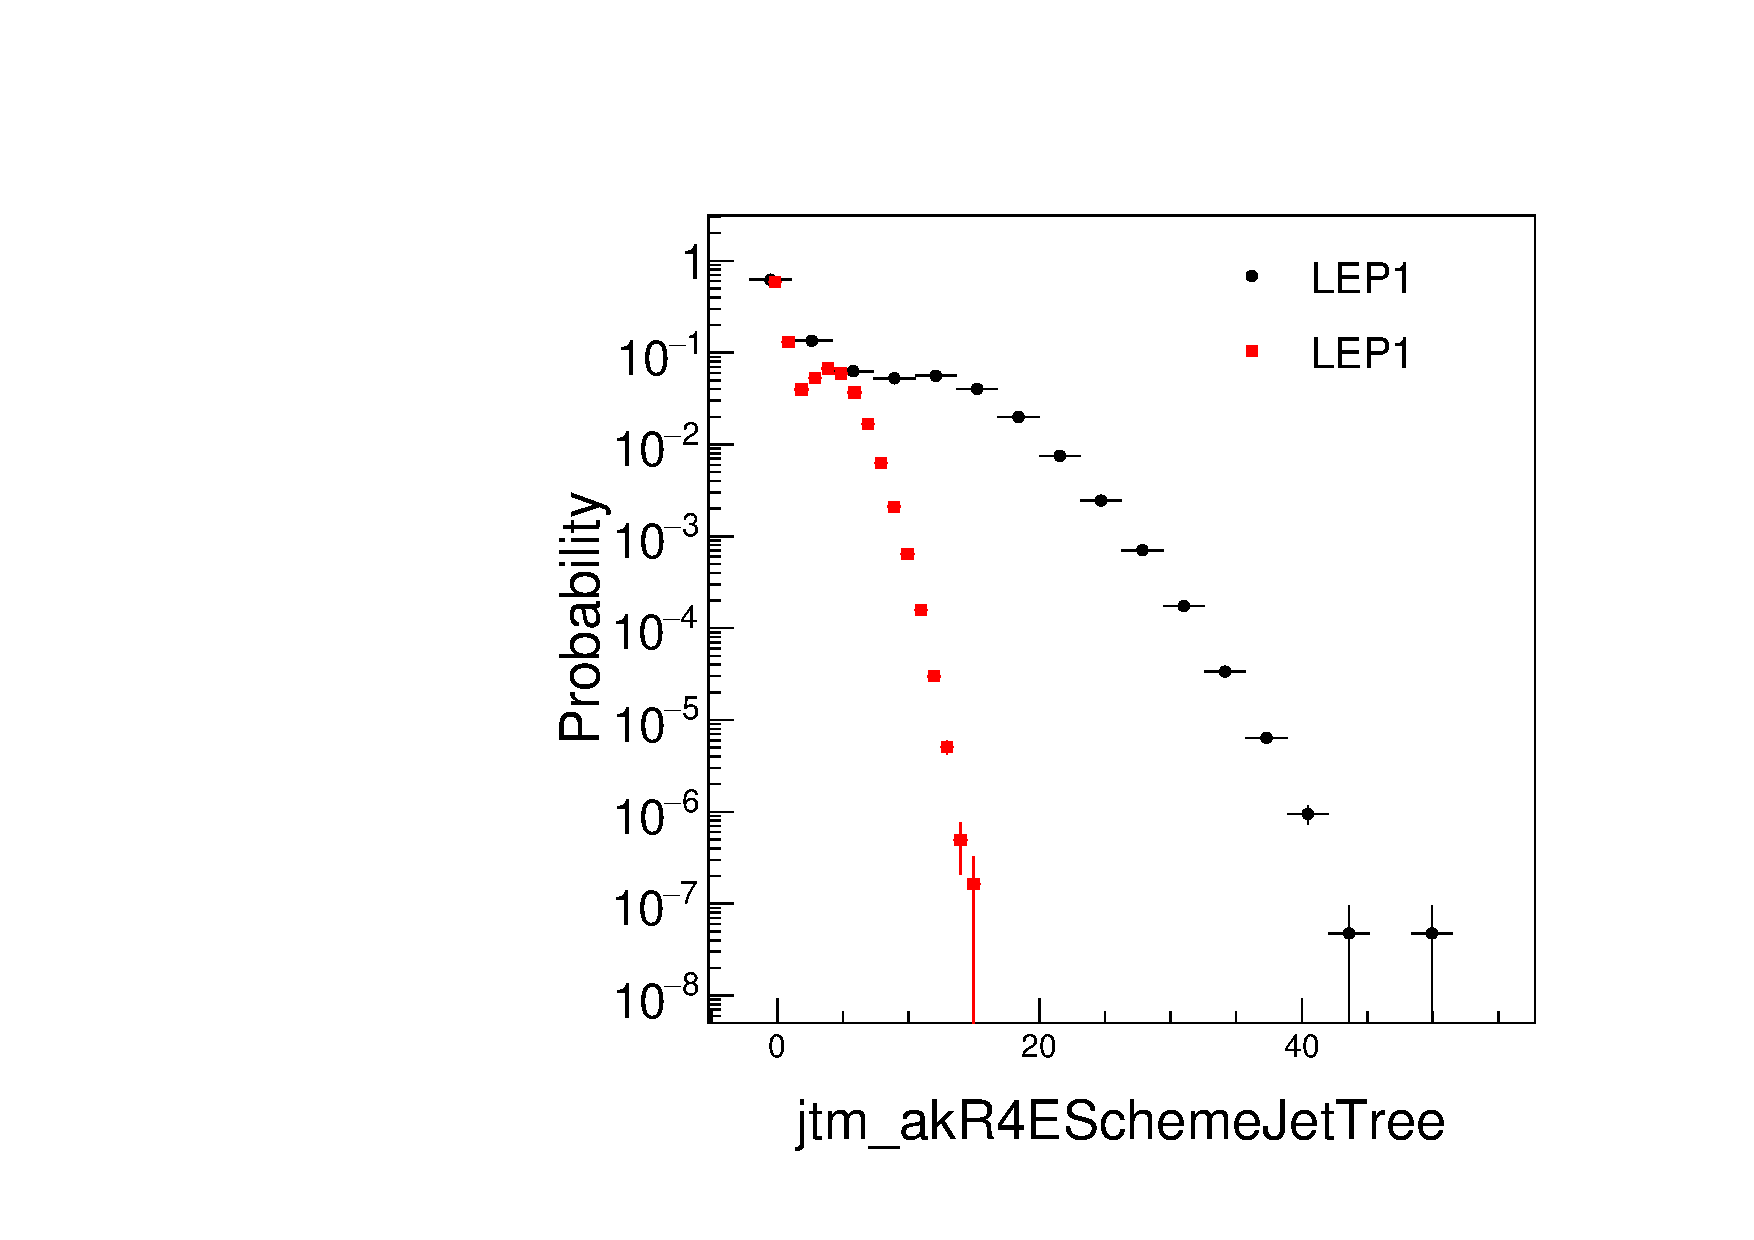
\includegraphics[width=.25\textwidth]{images/DQC/LEP1MC/jtm_akR4ESchemeJetTree.pdf}}\hfill
\subfloat{\label{sfig:b}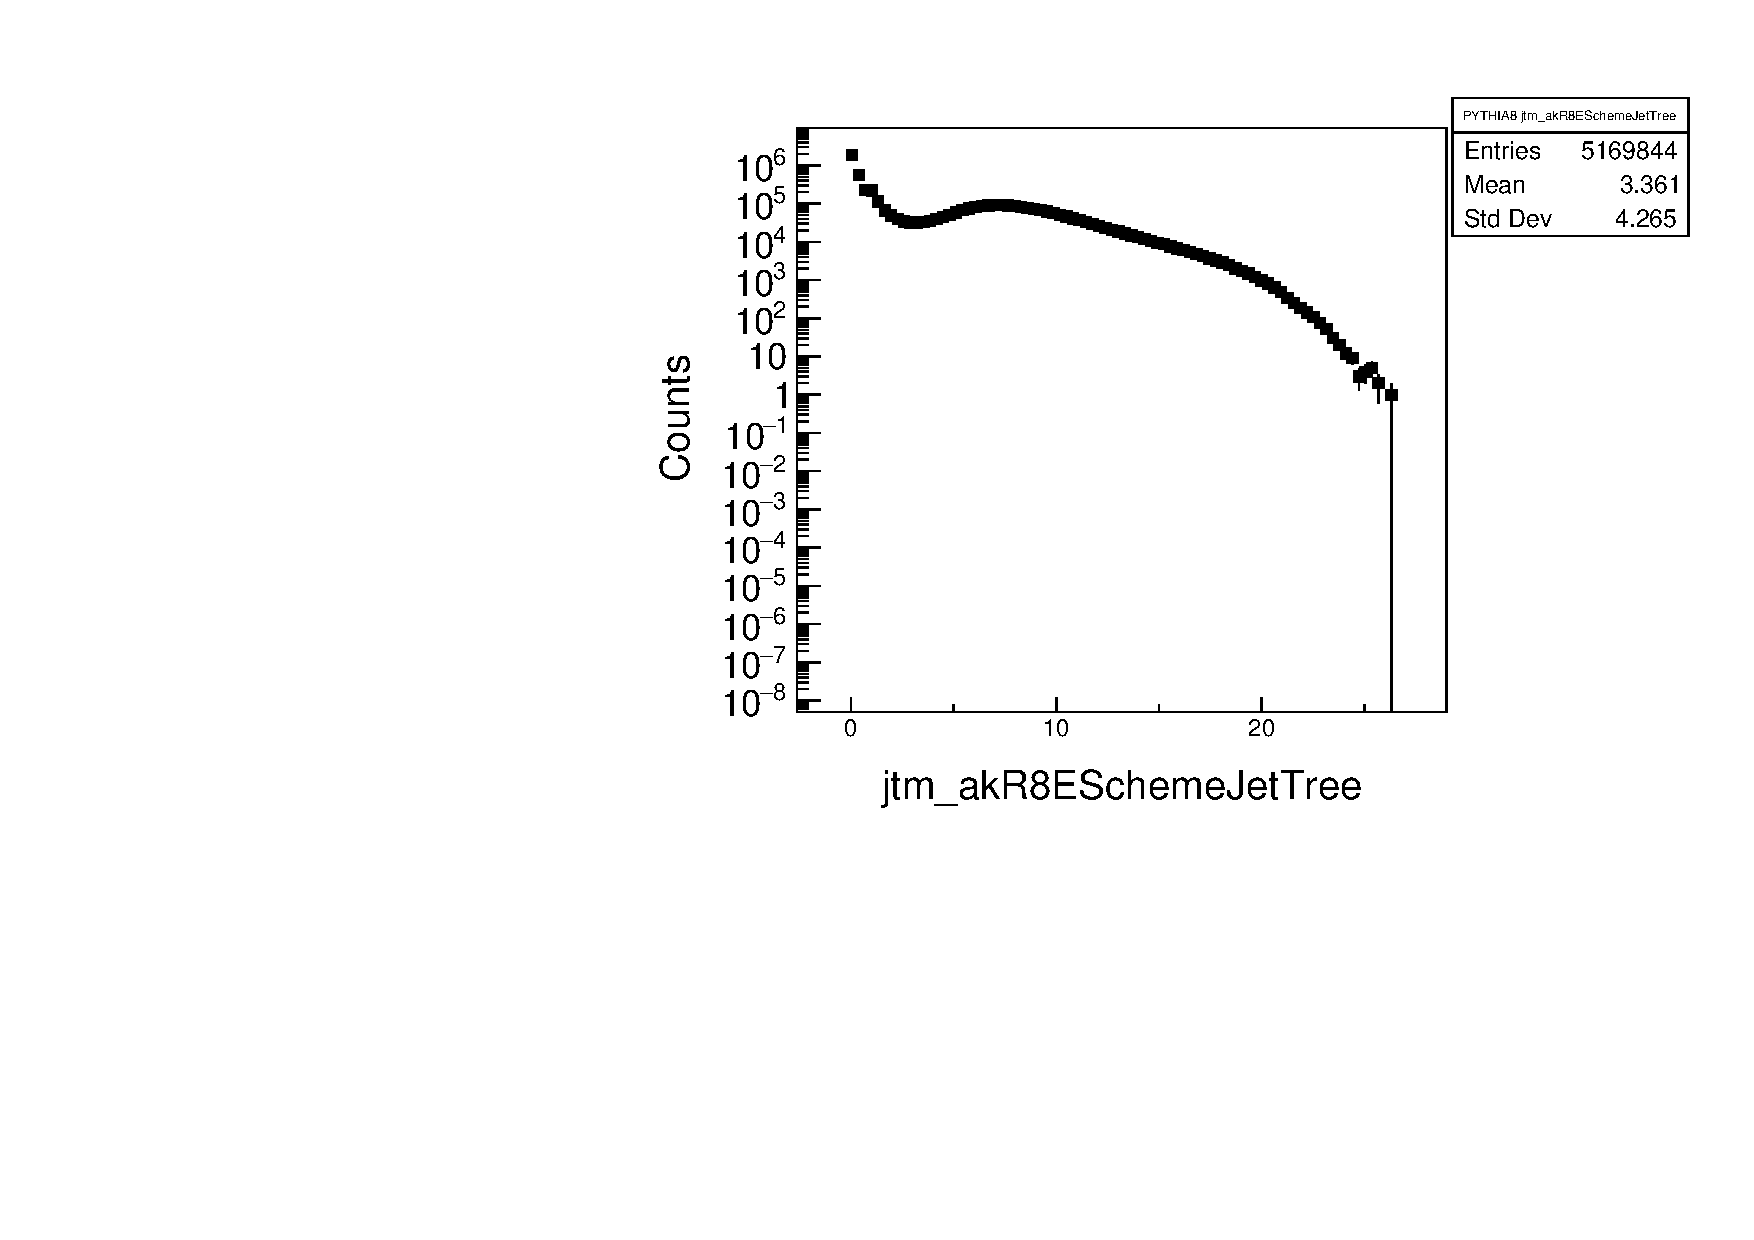
\includegraphics[width=.25\textwidth]{images/DQC/LEP1MC/jtm_akR8ESchemeJetTree.pdf}}\hfill
\subfloat{\label{sfig:c}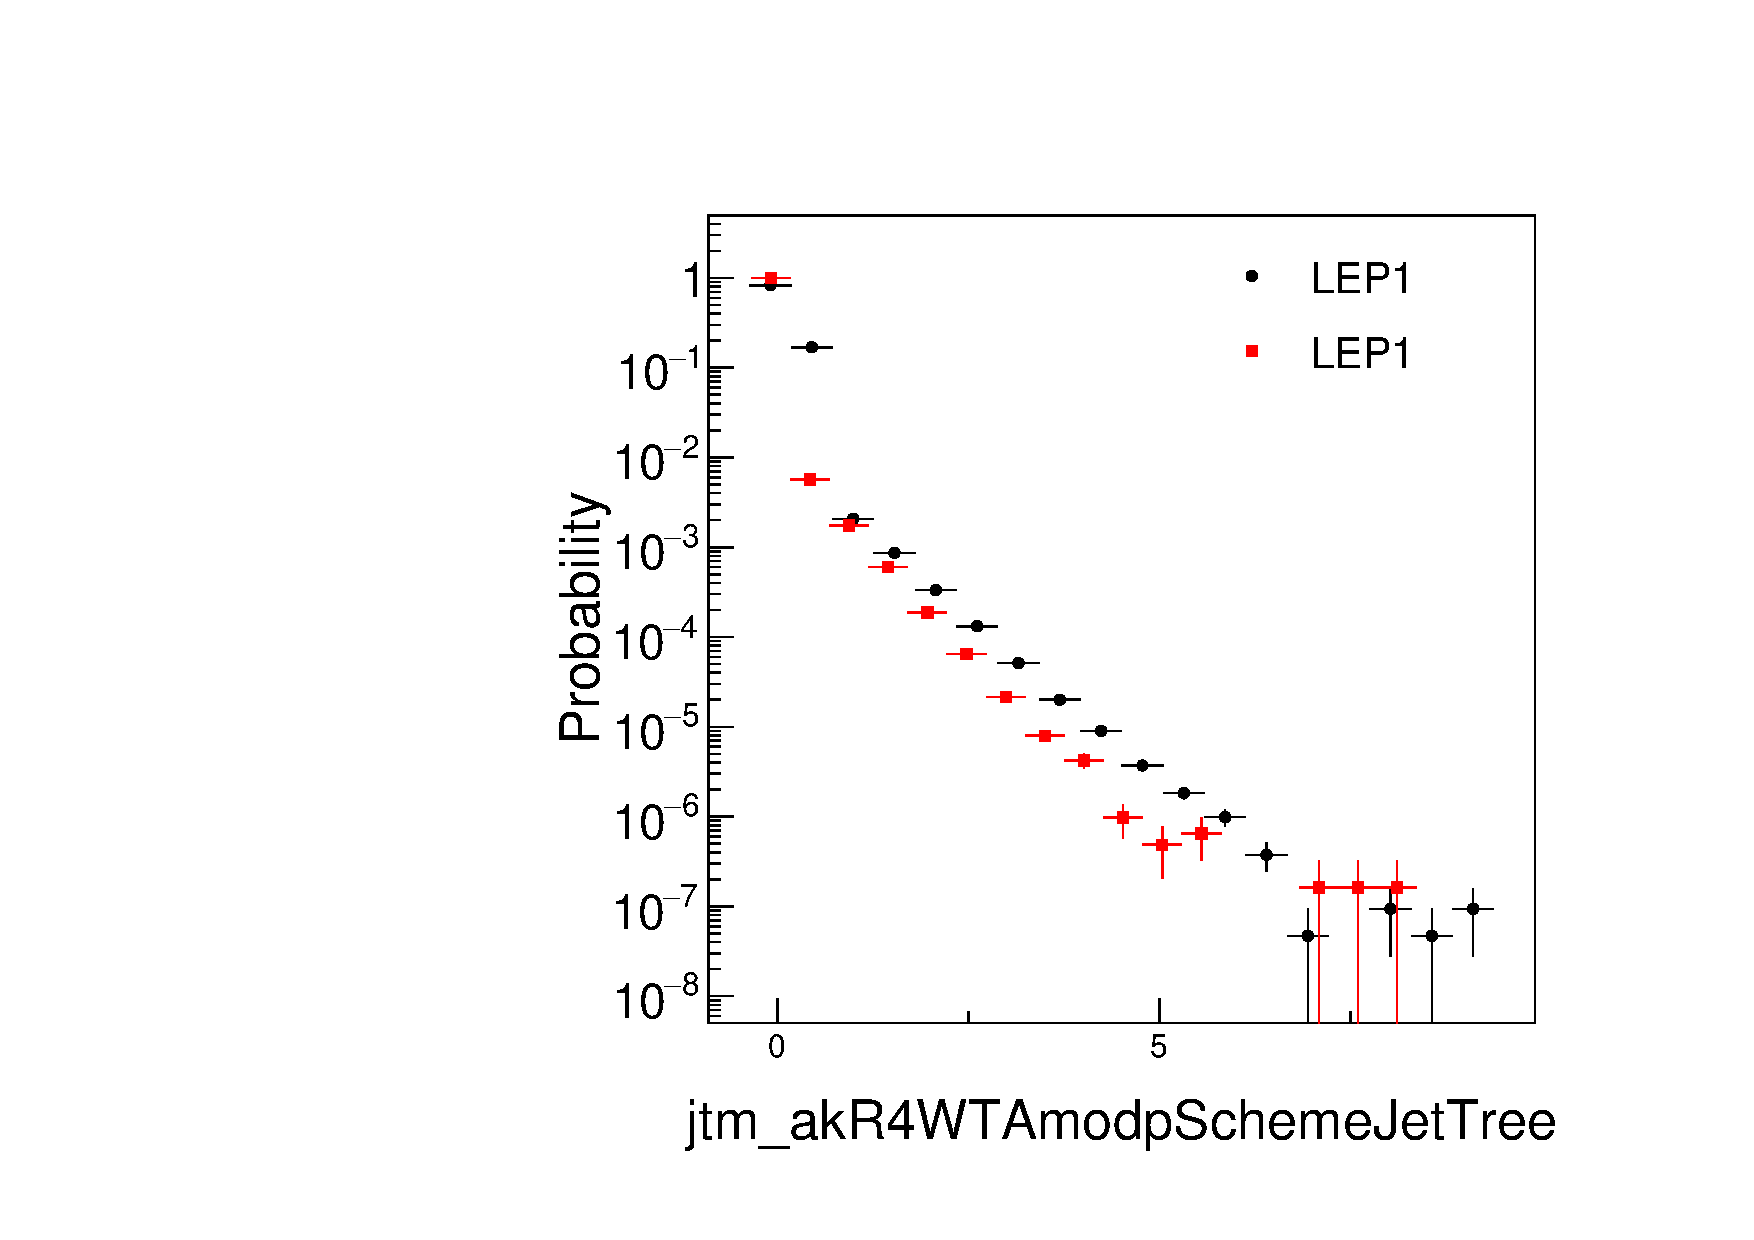
\includegraphics[width=.25\textwidth]{images/DQC/LEP1MC/jtm_akR4WTAmodpSchemeJetTree.pdf}}\hfill
\subfloat{\label{sfig:d}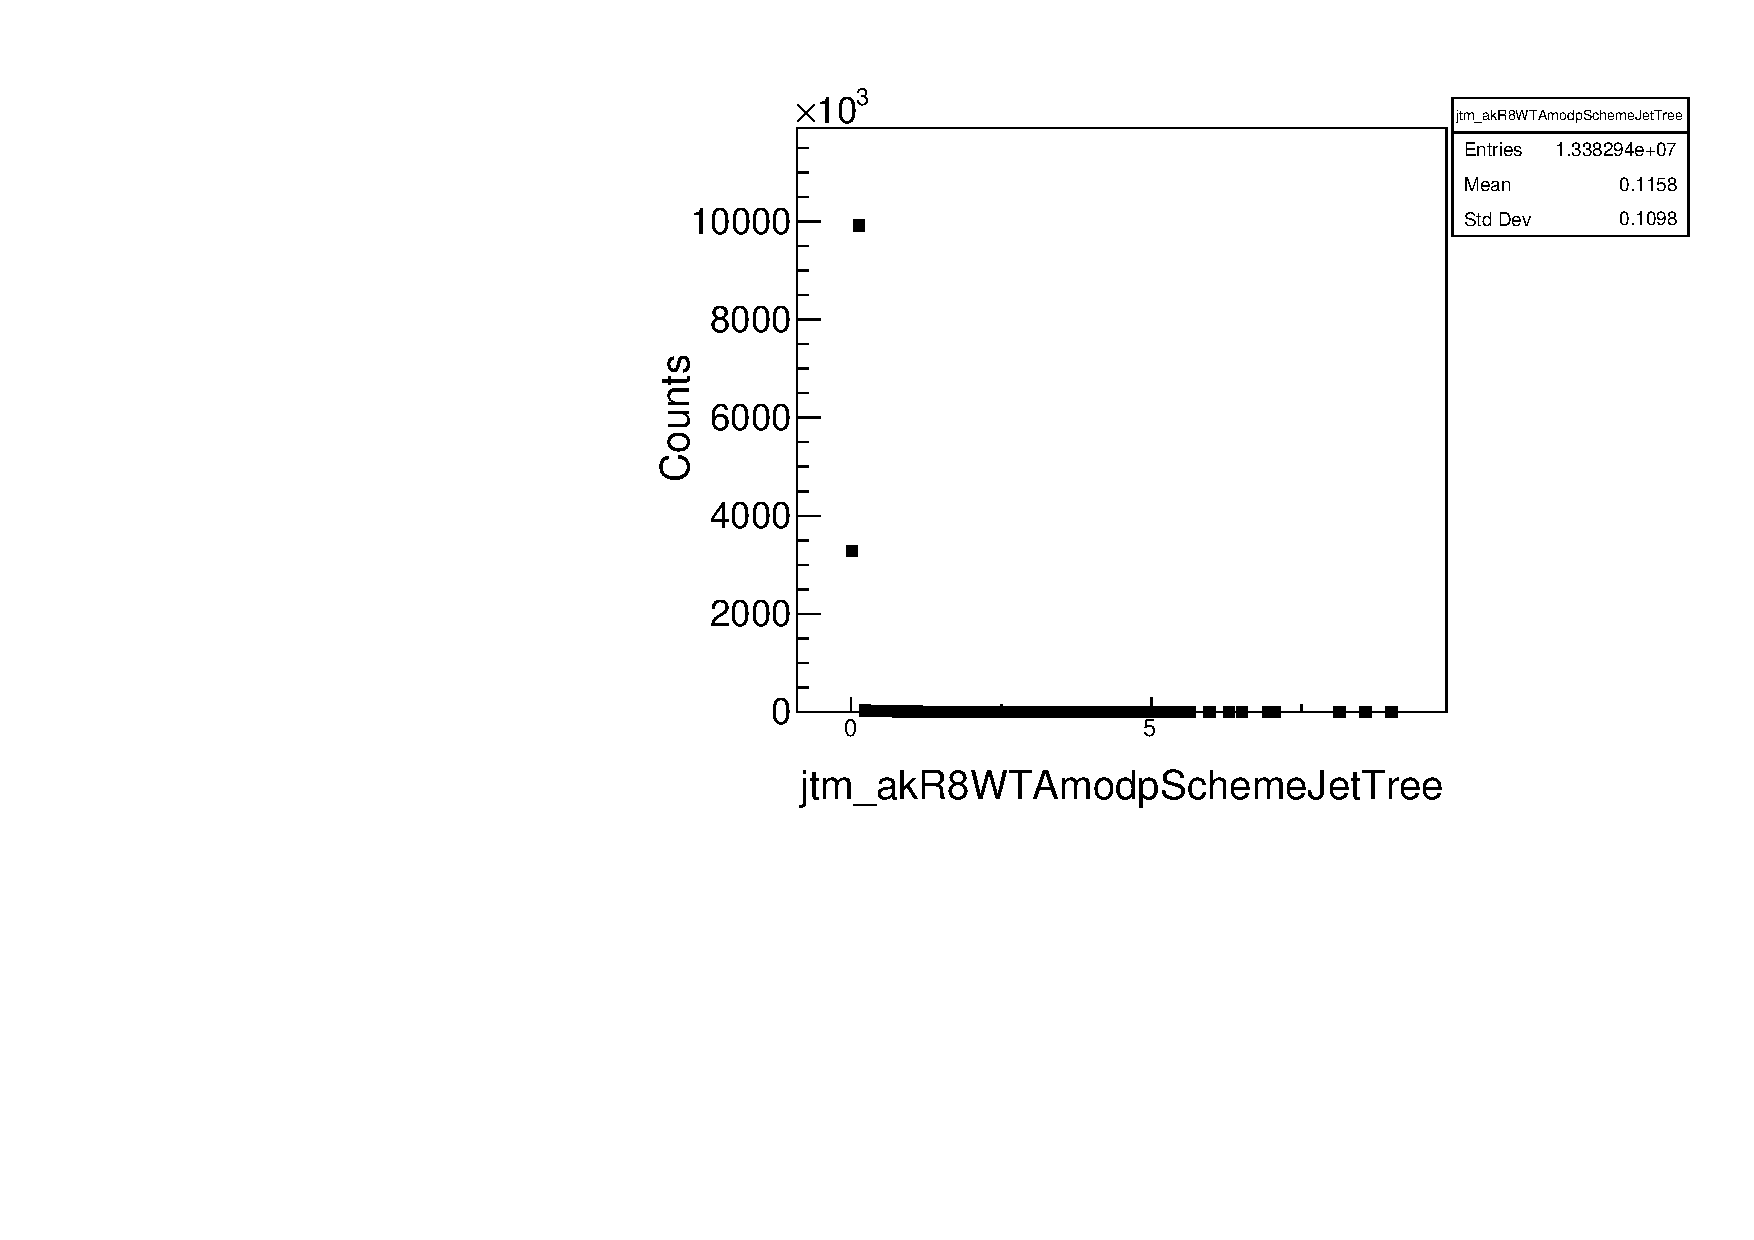
\includegraphics[width=.25\textwidth]{images/DQC/LEP1MC/jtm_akR8WTAmodpSchemeJetTree.pdf}}\hfill %row end
\subfloat{\label{sfig:e}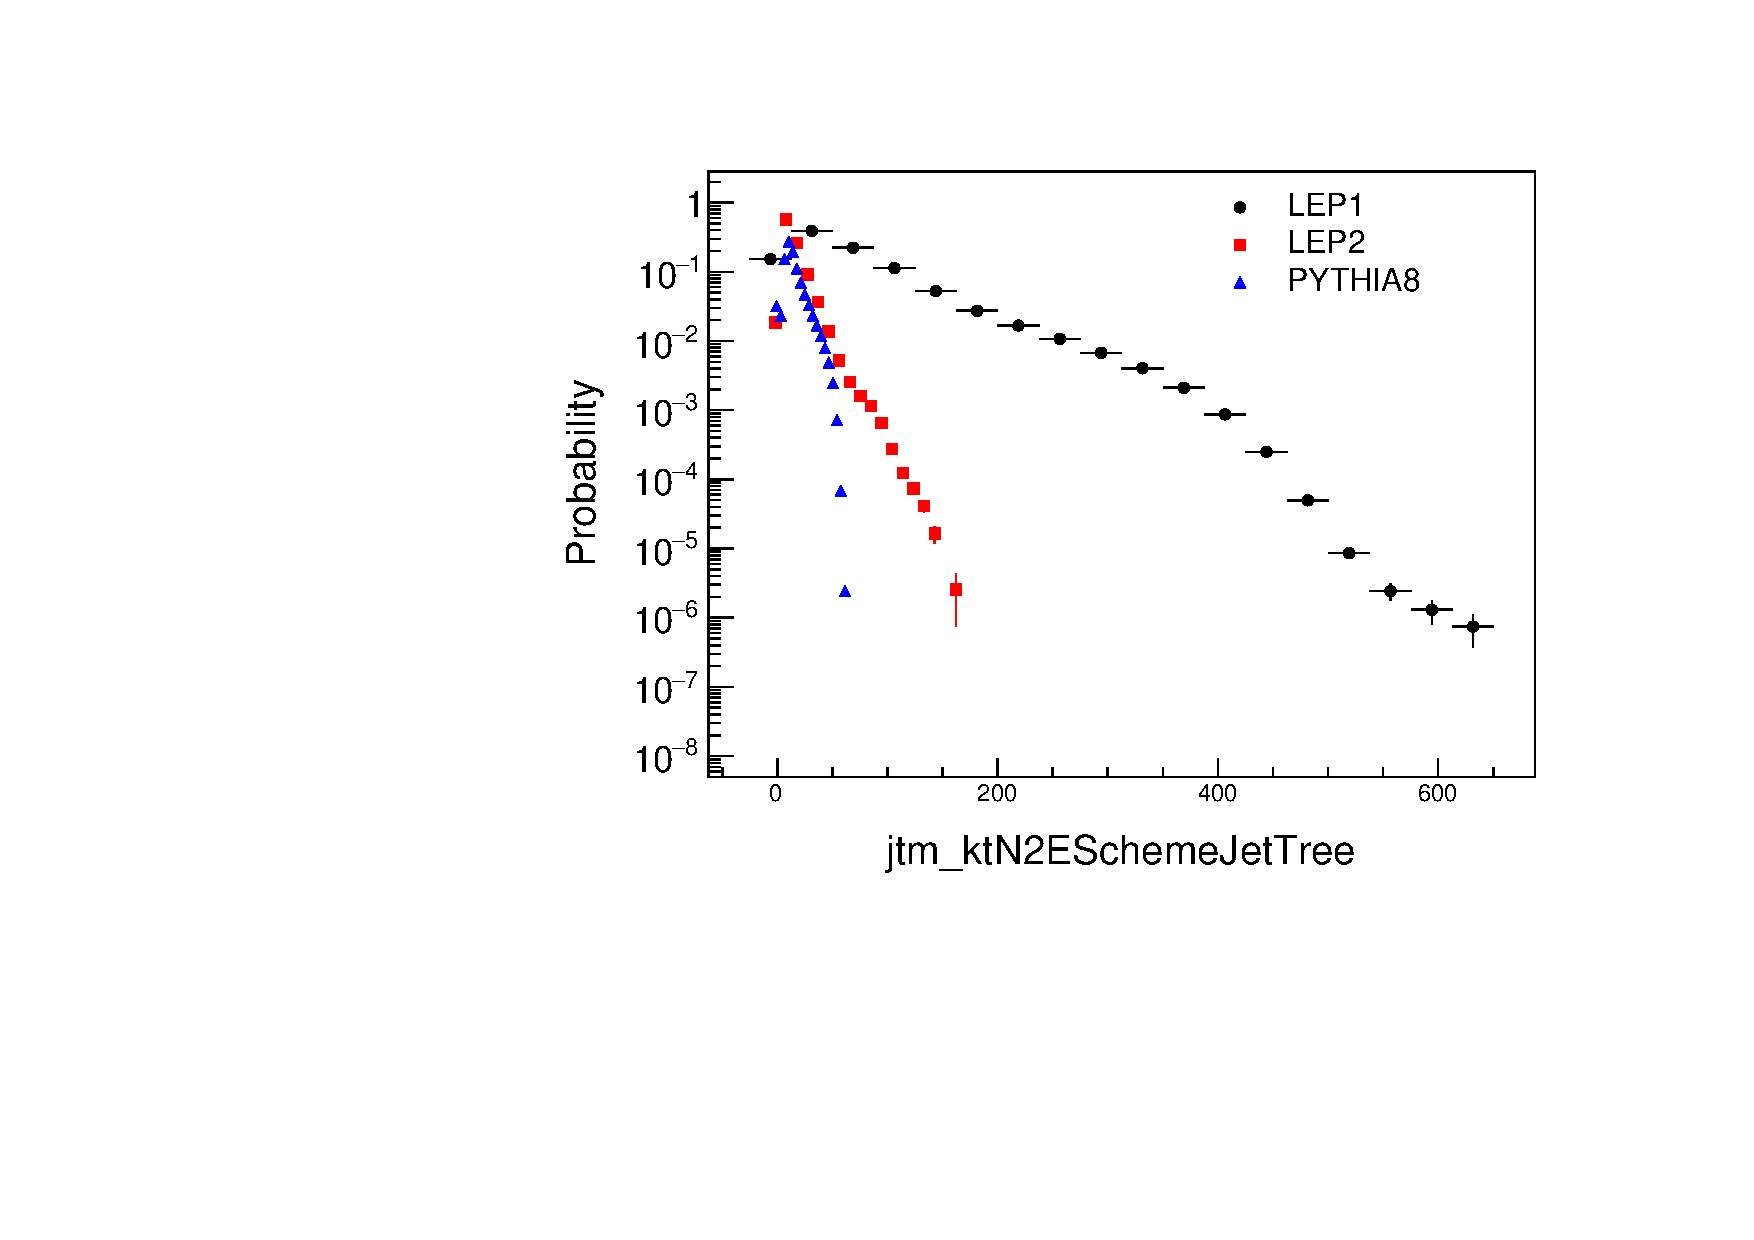
\includegraphics[width=.25\textwidth]{images/DQC/LEP1MC/jtm_ktN2ESchemeJetTree.pdf}}\hfill
\subfloat{\label{sfig:f}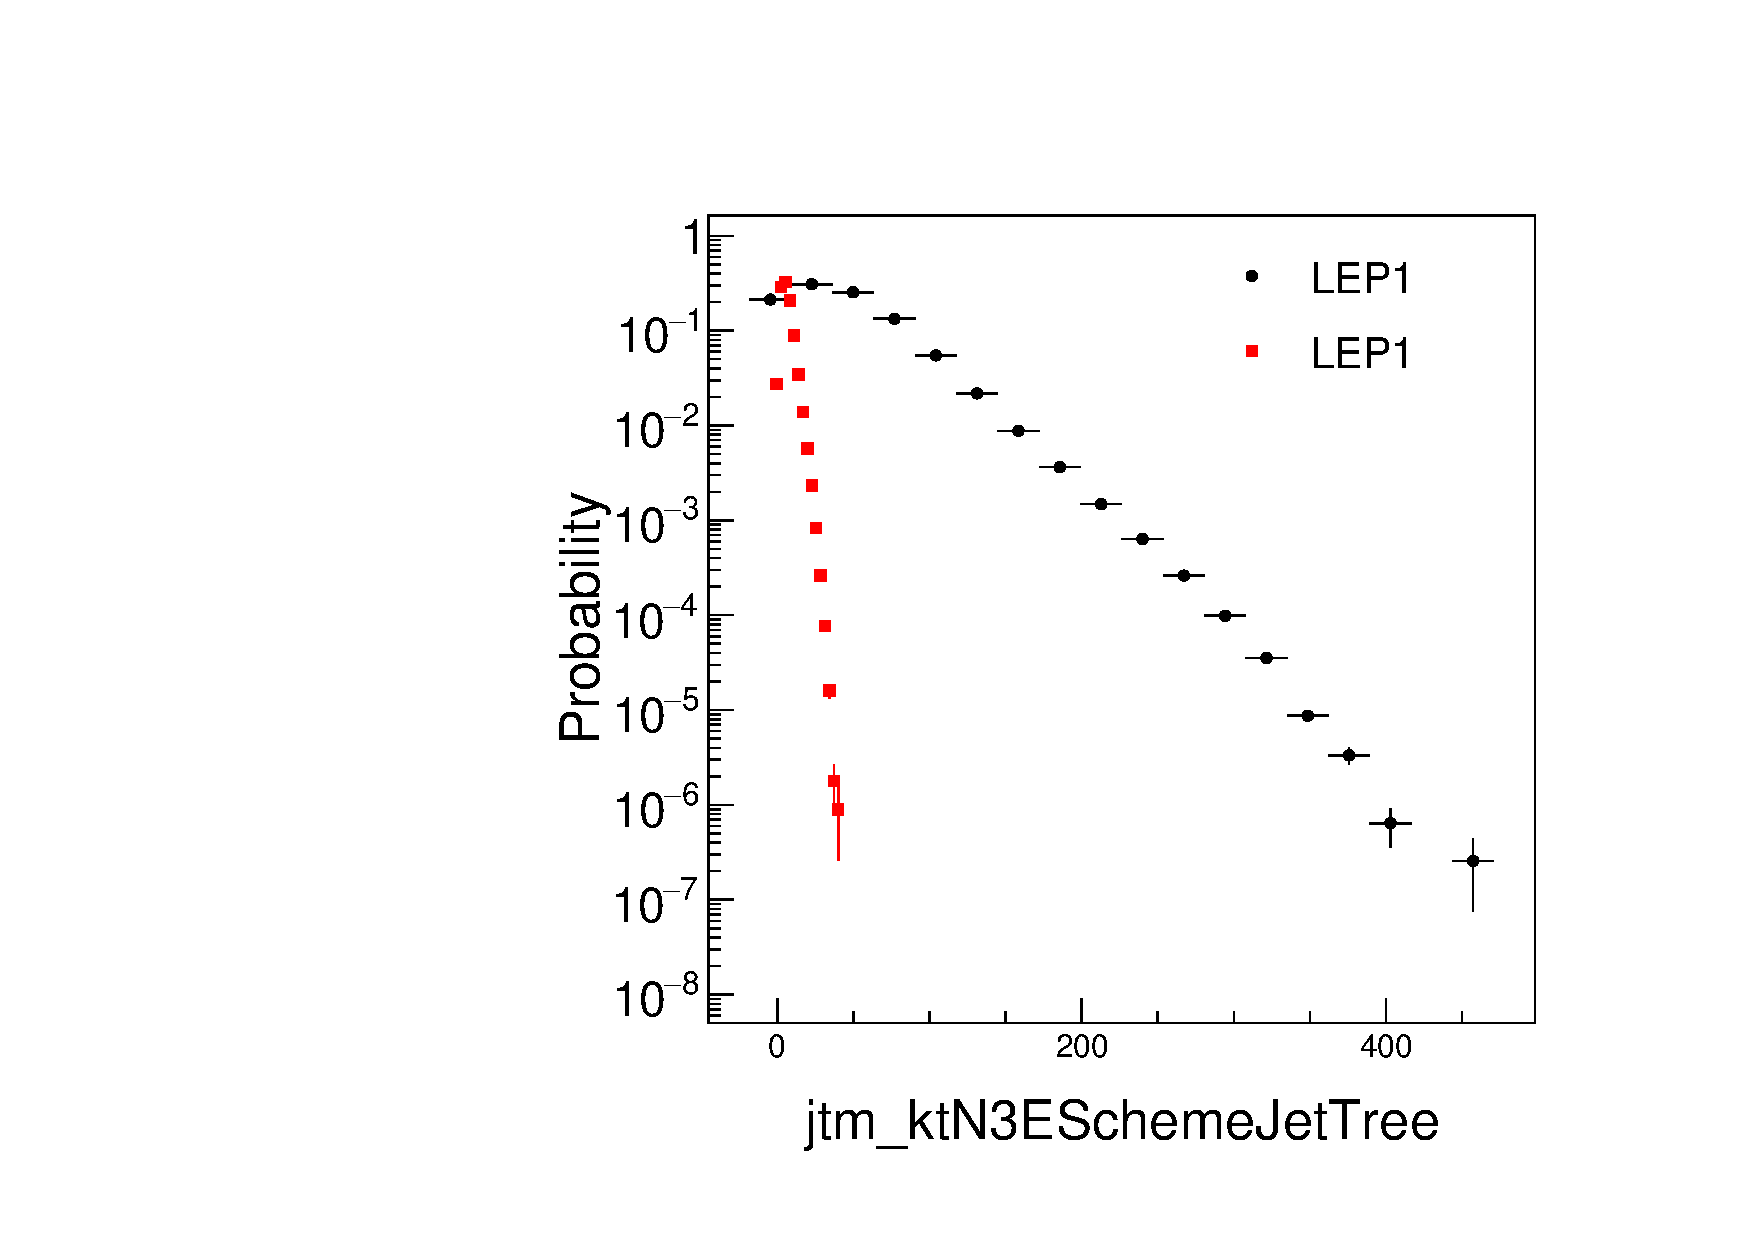
\includegraphics[width=.25\textwidth]{images/DQC/LEP1MC/jtm_ktN3ESchemeJetTree.pdf}}\hfill
\subfloat{\label{sfig:g}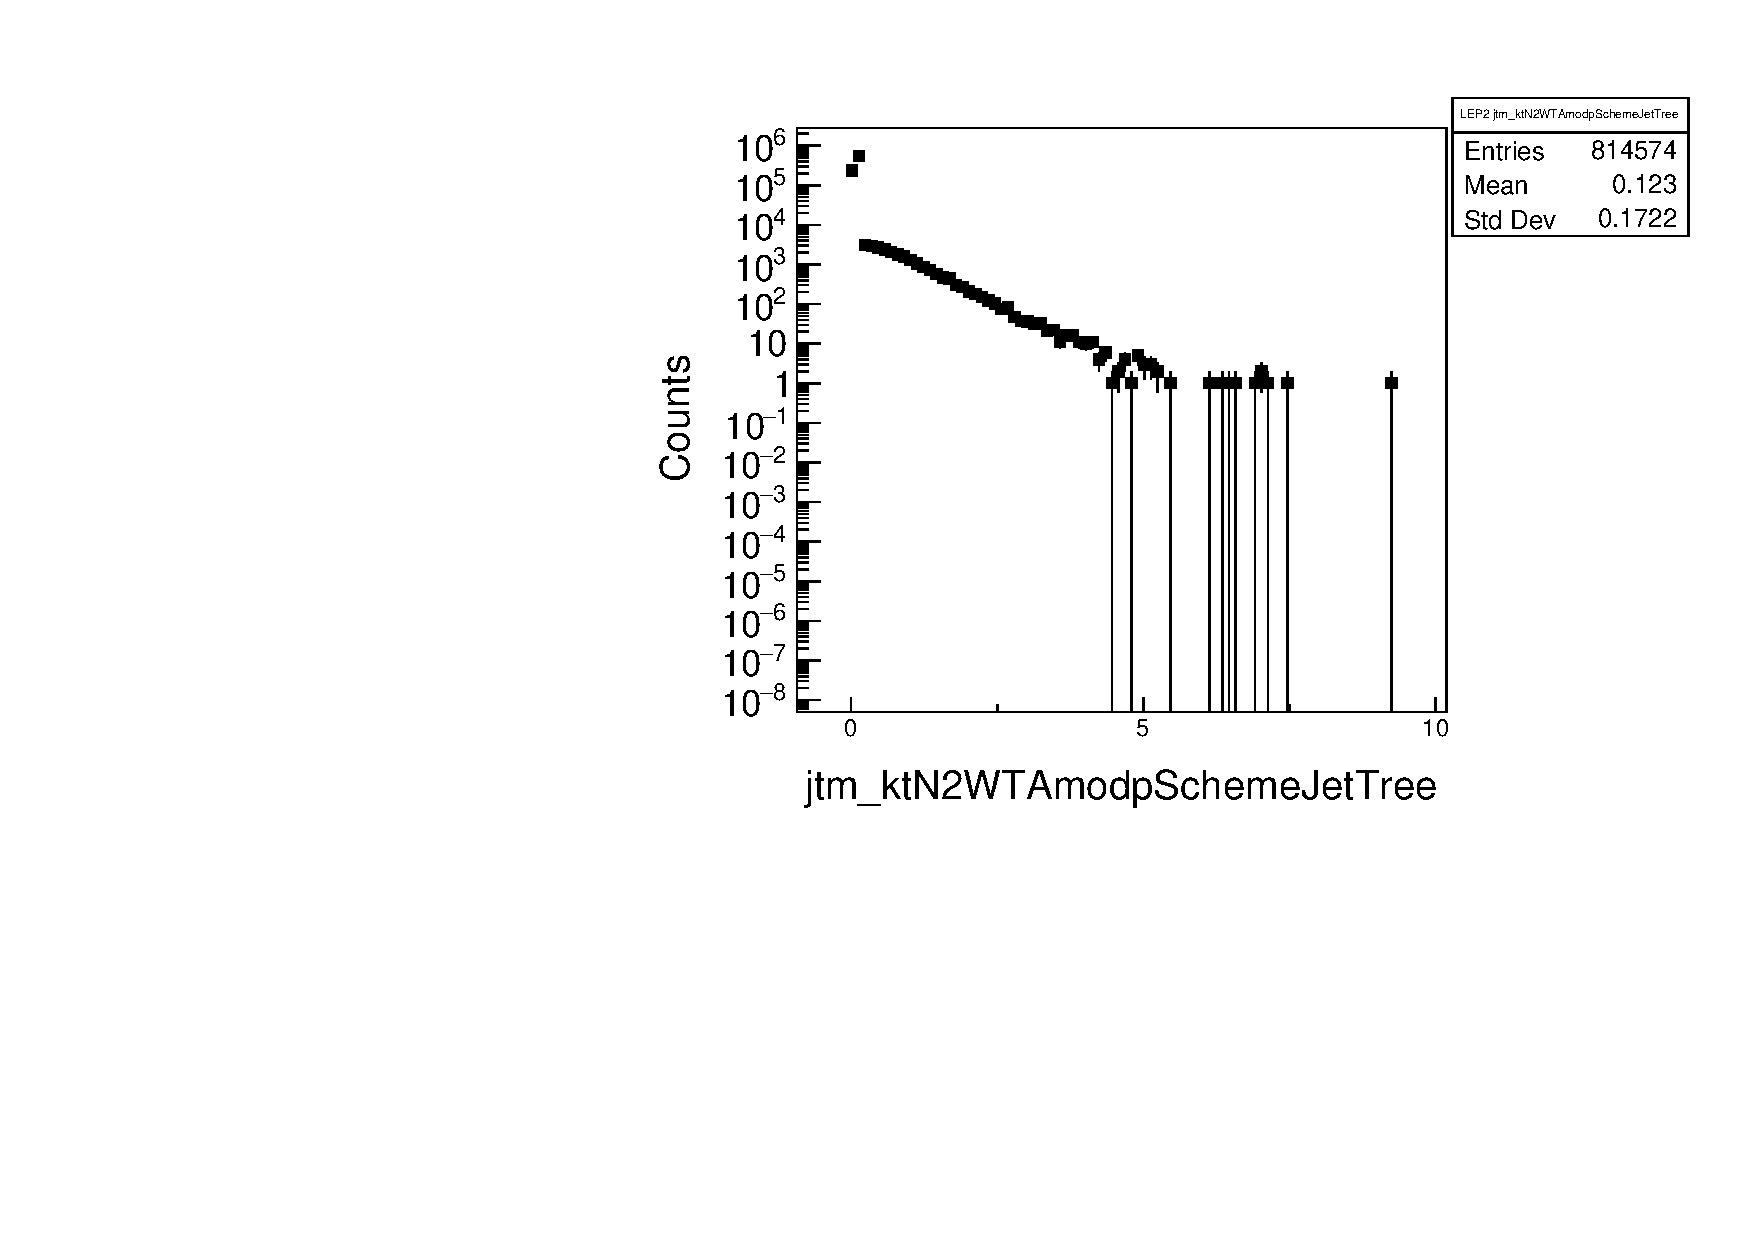
\includegraphics[width=.25\textwidth]{images/DQC/LEP1MC/jtm_ktN2WTAmodpSchemeJetTree.pdf}}\hfill
\subfloat{\label{sfig:h}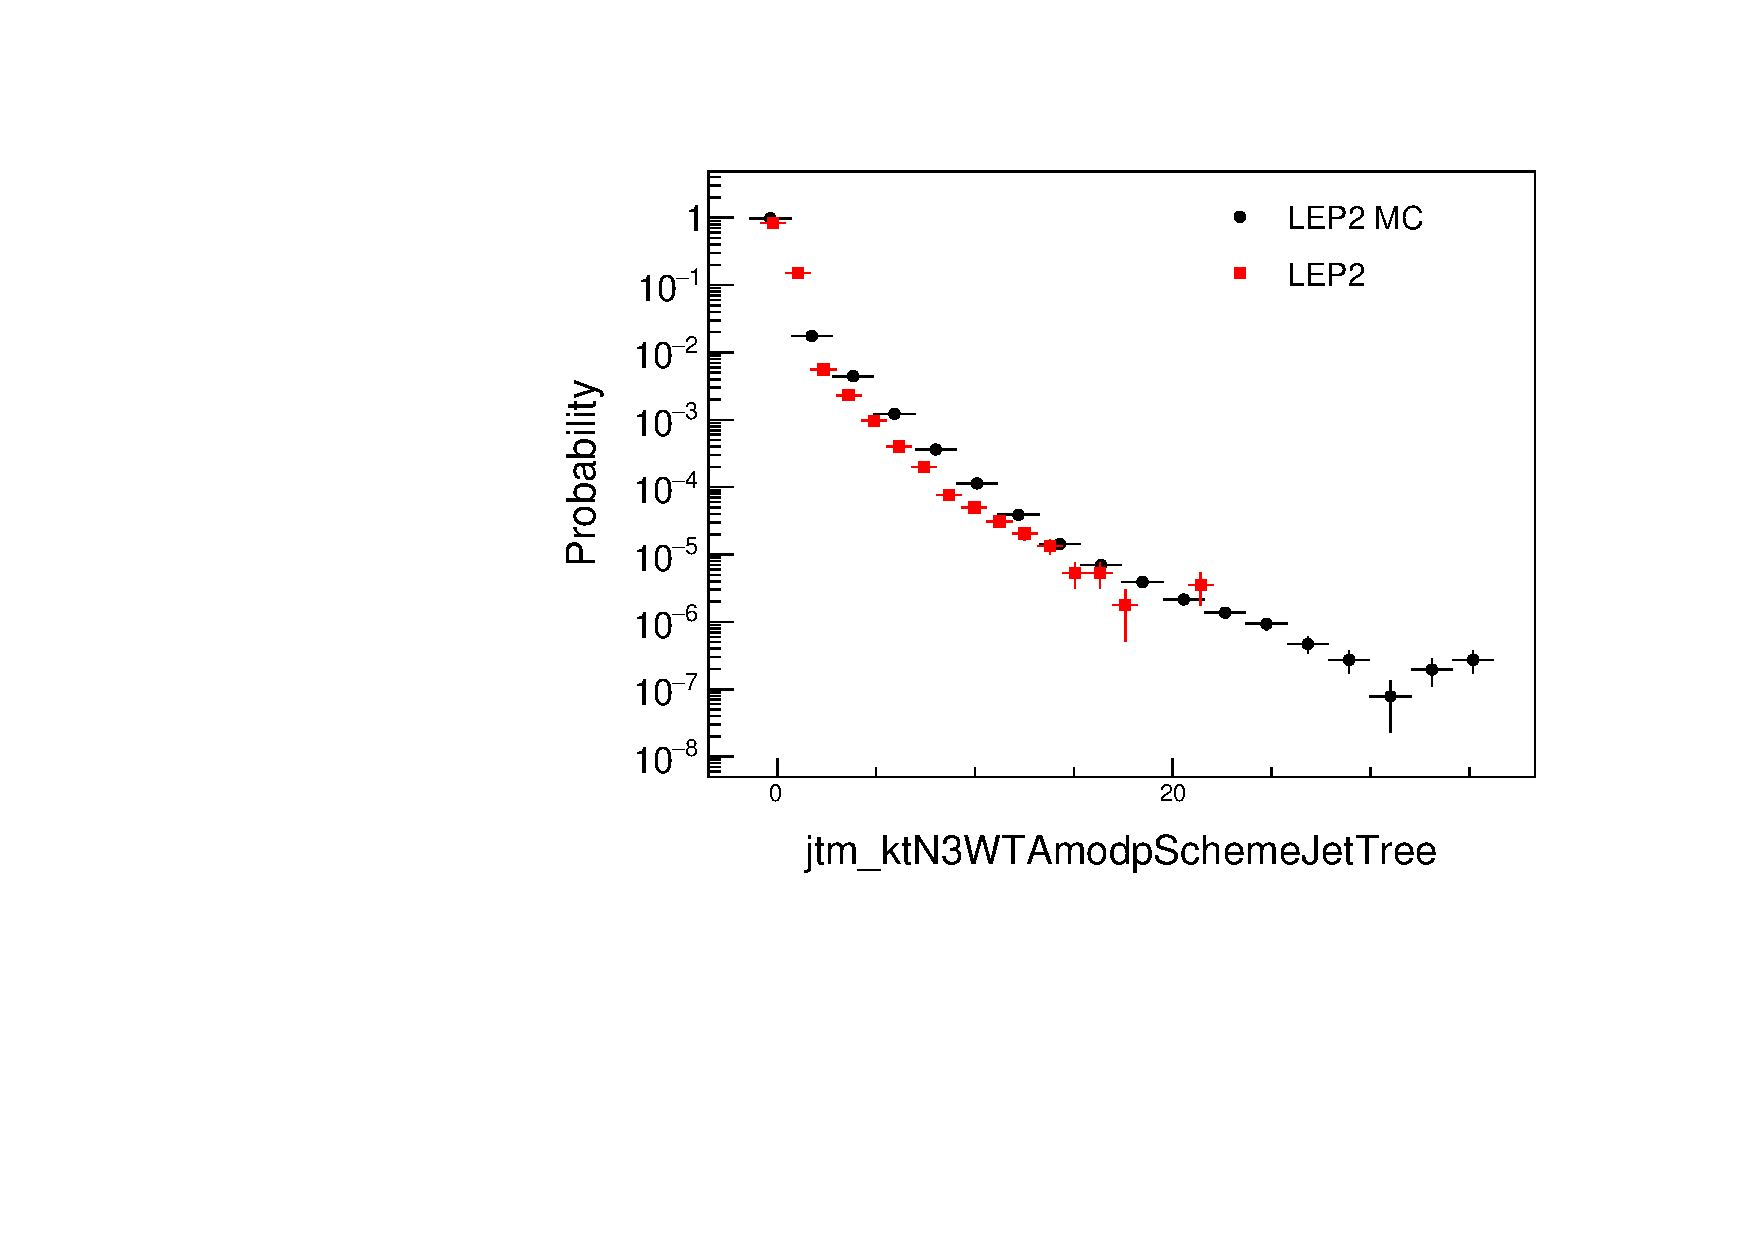
\includegraphics[width=.25\textwidth]{images/DQC/LEP1MC/jtm_ktN3WTAmodpSchemeJetTree.pdf}}\hfill
\caption{LEP1 vs LEP1 MC Jet mass distributions. Top row: anti-$k_t$, left to right: $R=0.4$, $E$ scheme; $R=0.8$, $E$ scheme; $R=0.4$, WTA mod p scheme; $R=0.8$, WTA mod p scheme. Bottom row: $k_t$, left to right: $N=2$, $E$ scheme; $N=3$, $E$ scheme; $N=2$, WTA mod p scheme; $N=3$; WTA mod p scheme.}  
\end{figure}

\begin{figure}[H]
\centering
\subfloat{\label{sfig:a}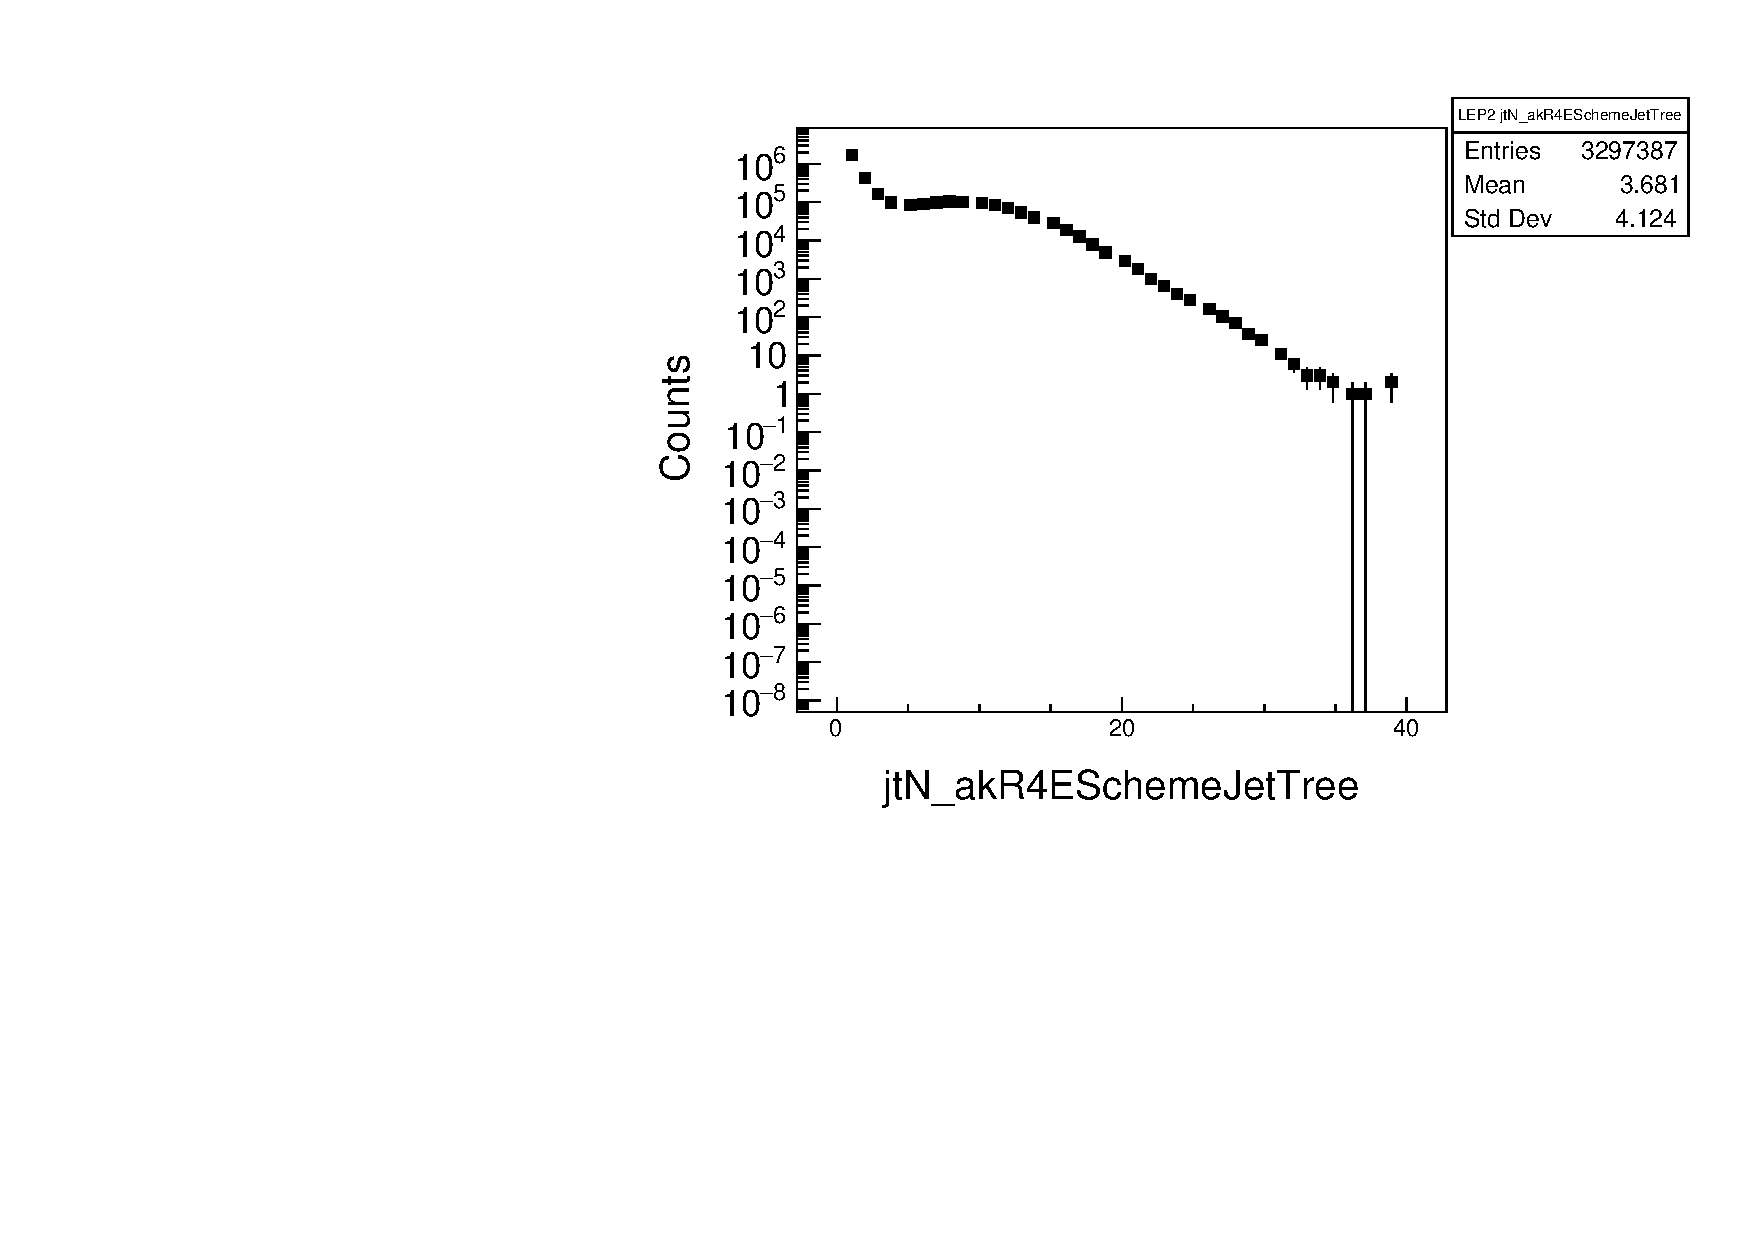
\includegraphics[width=.25\textwidth]{images/DQC/LEP1MC/jtN_akR4ESchemeJetTree.pdf}}\hfill
\subfloat{\label{sfig:b}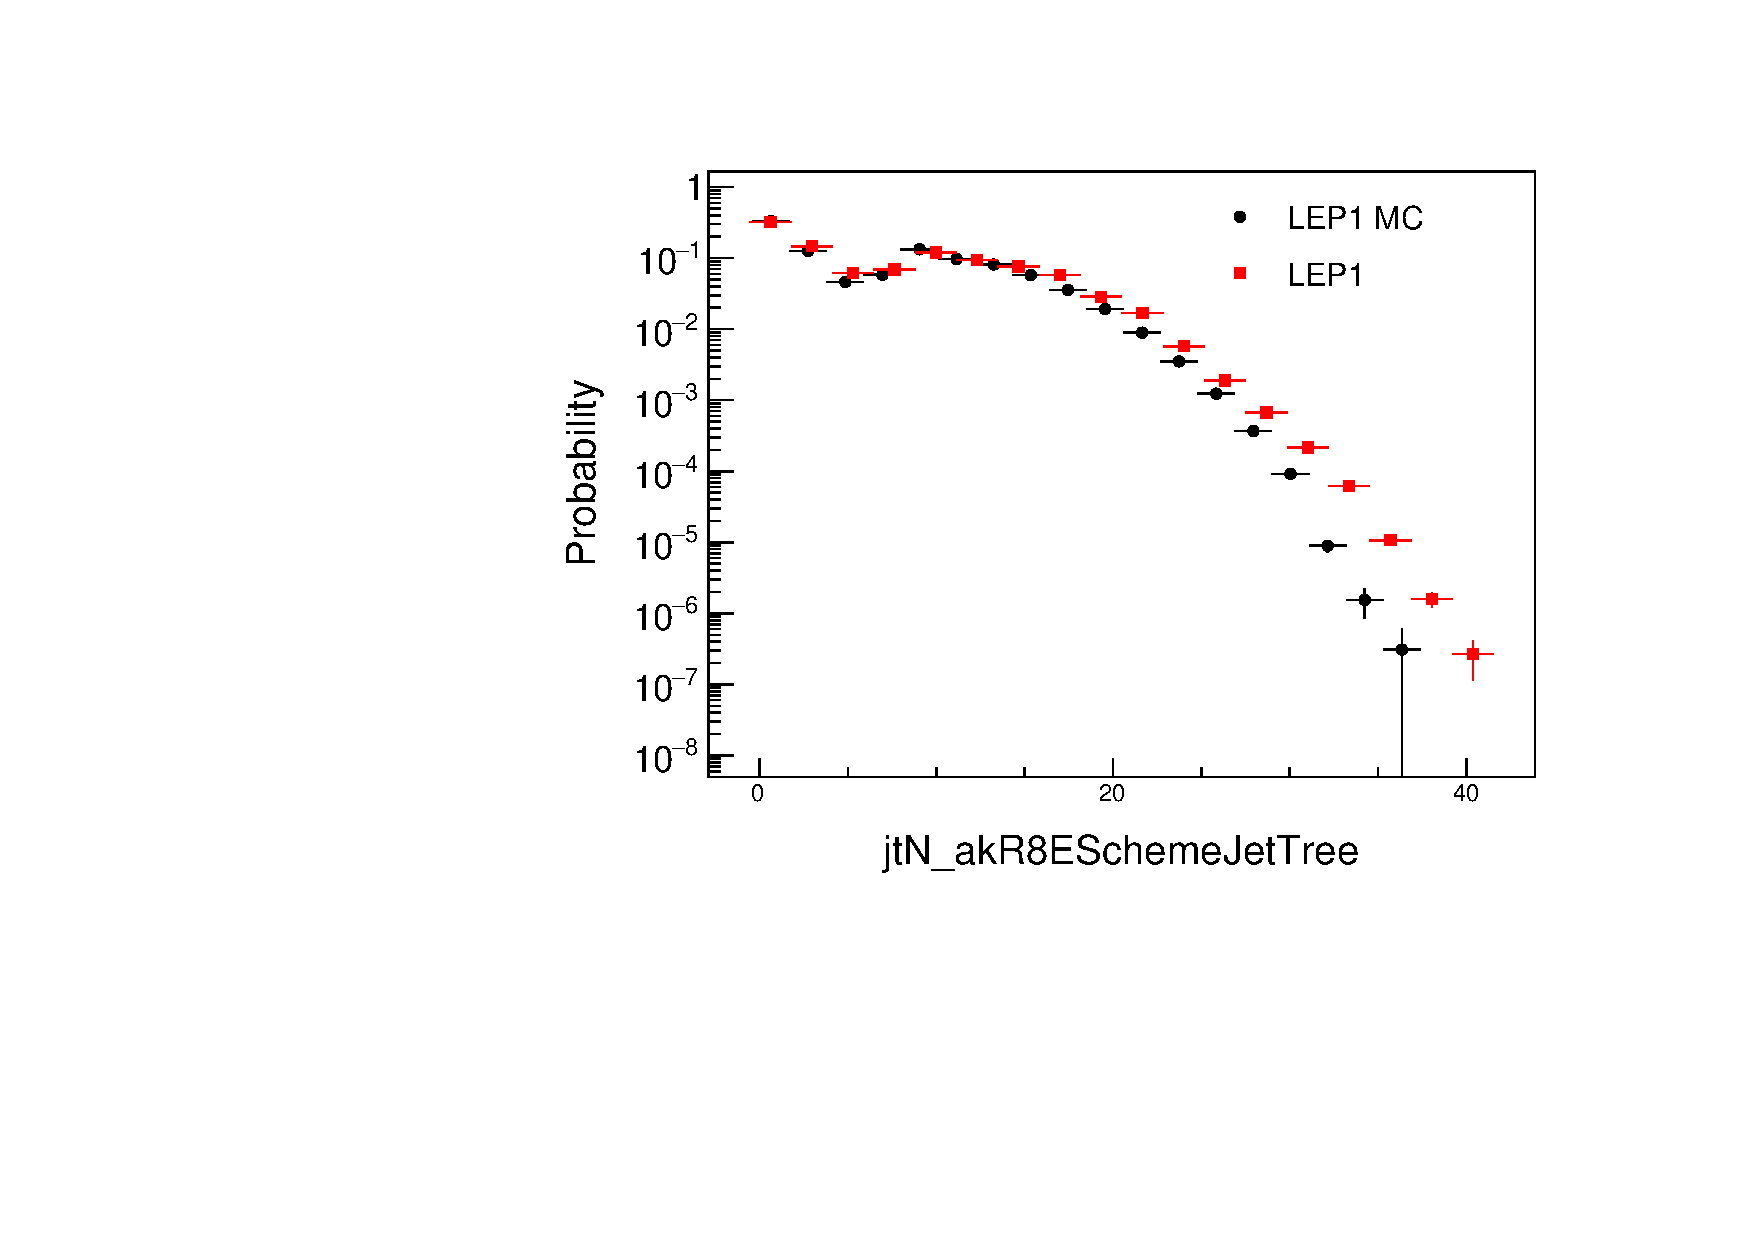
\includegraphics[width=.25\textwidth]{images/DQC/LEP1MC/jtN_akR8ESchemeJetTree.pdf}}\hfill
\subfloat{\label{sfig:c}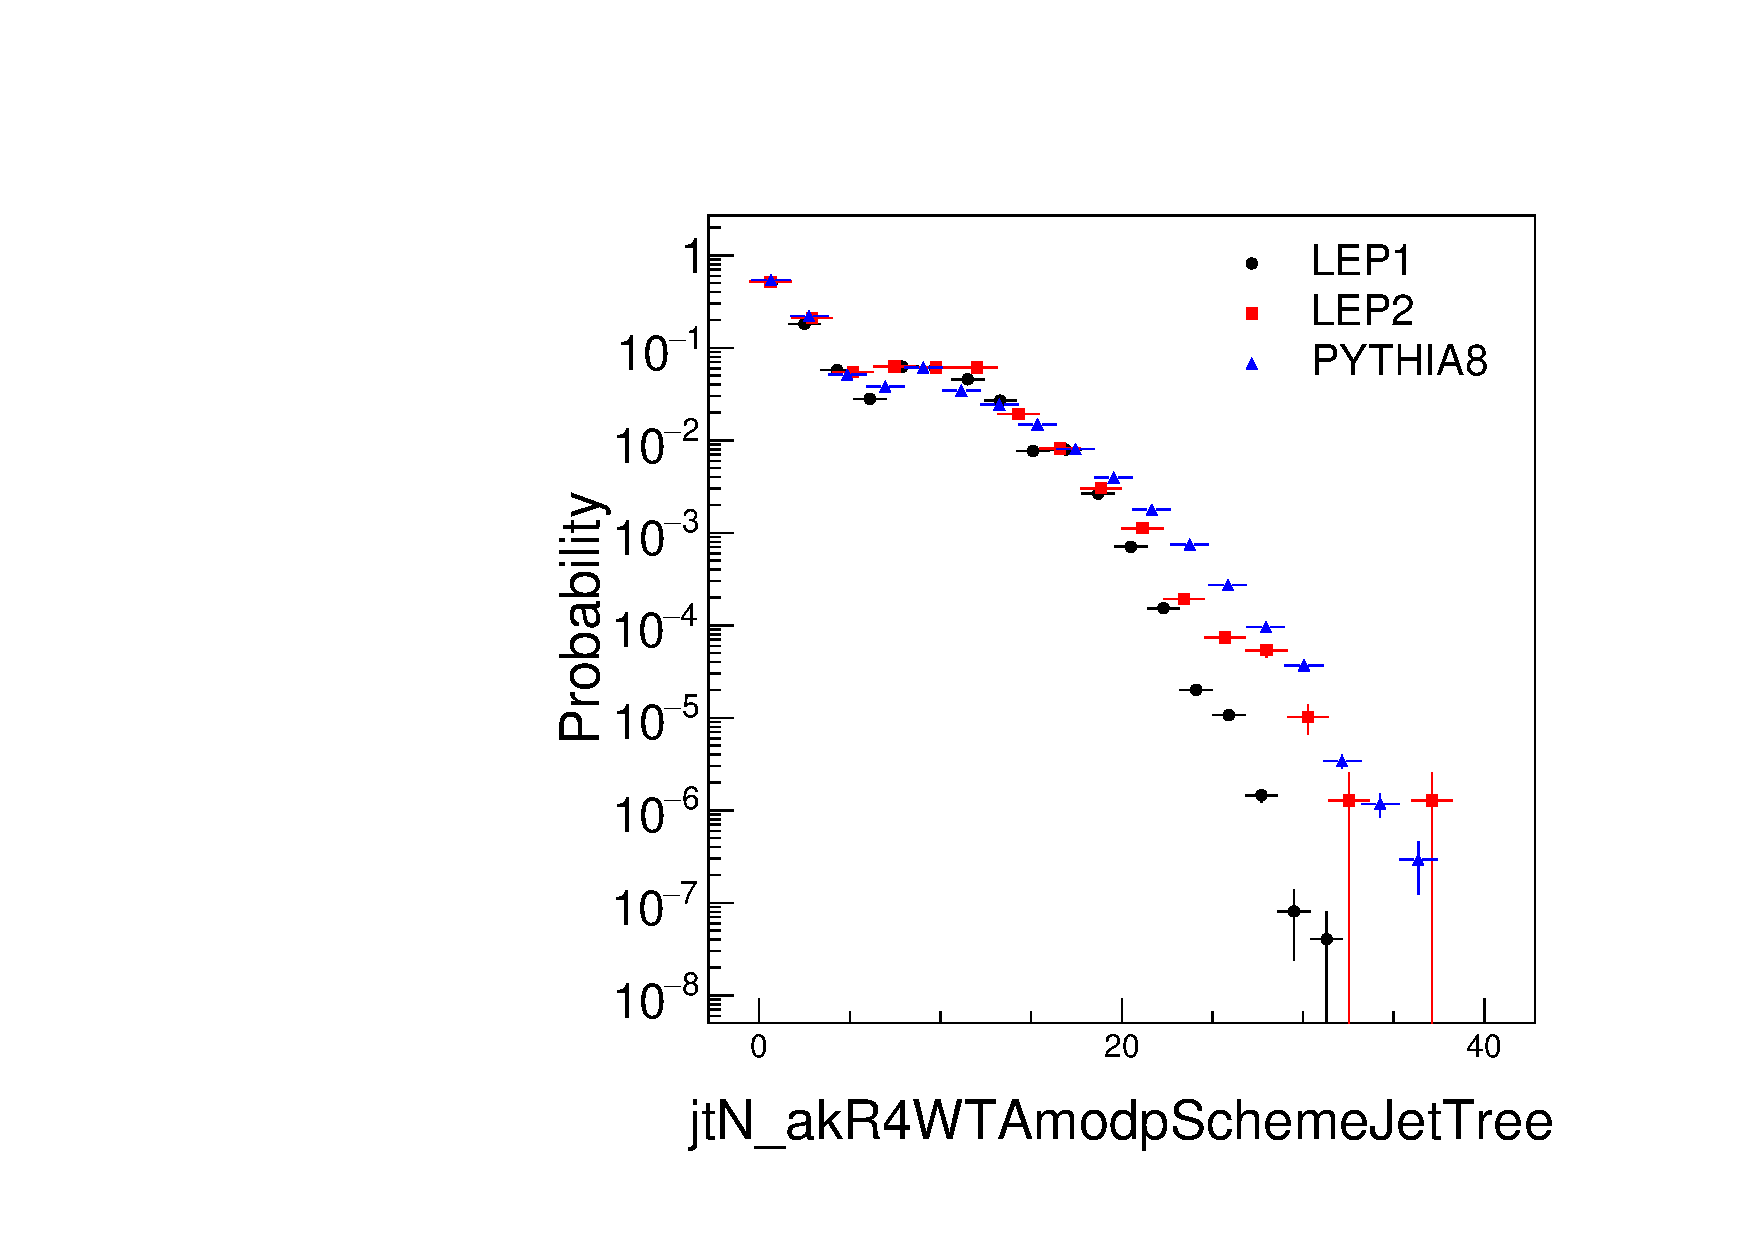
\includegraphics[width=.25\textwidth]{images/DQC/LEP1MC/jtN_akR4WTAmodpSchemeJetTree.pdf}}\hfill
\subfloat{\label{sfig:d}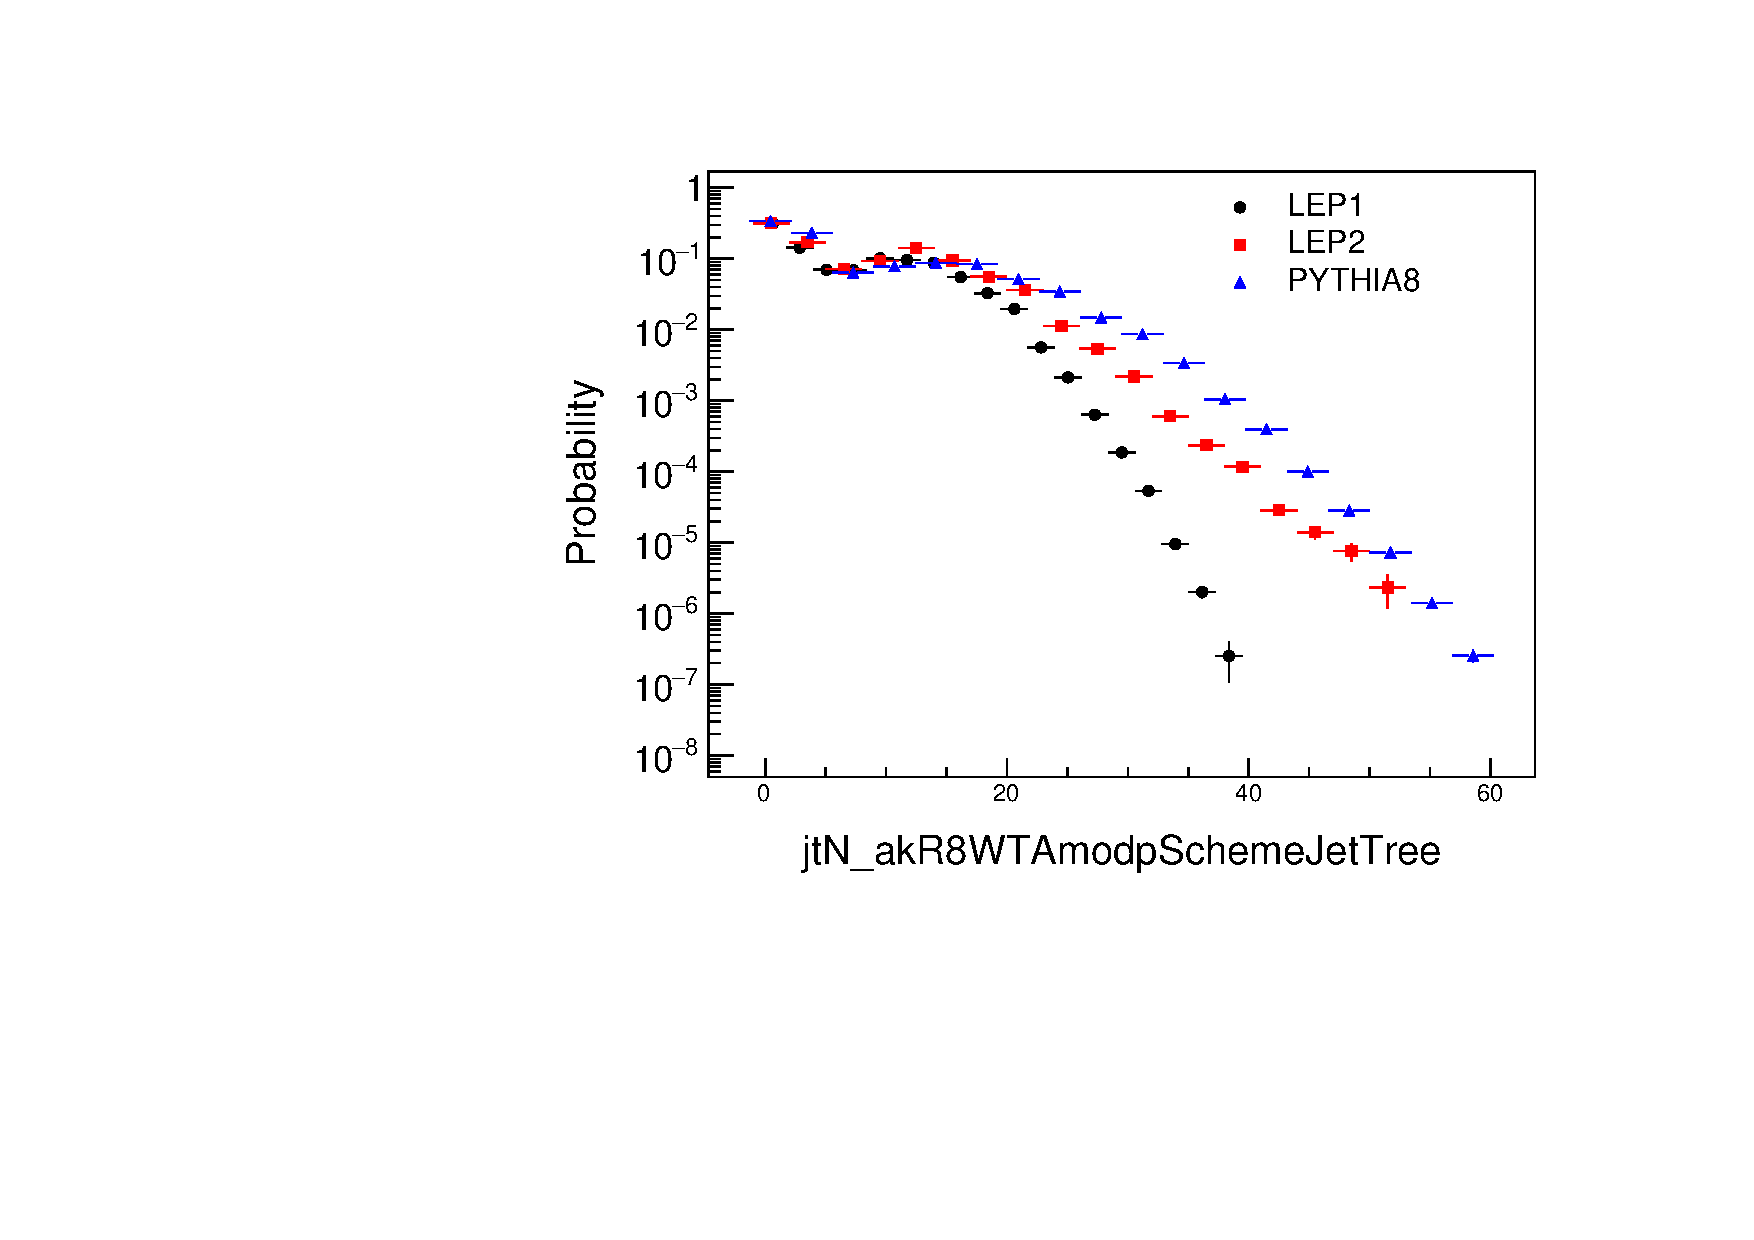
\includegraphics[width=.25\textwidth]{images/DQC/LEP1MC/jtN_akR8WTAmodpSchemeJetTree.pdf}}\hfill %row end
\subfloat{\label{sfig:e}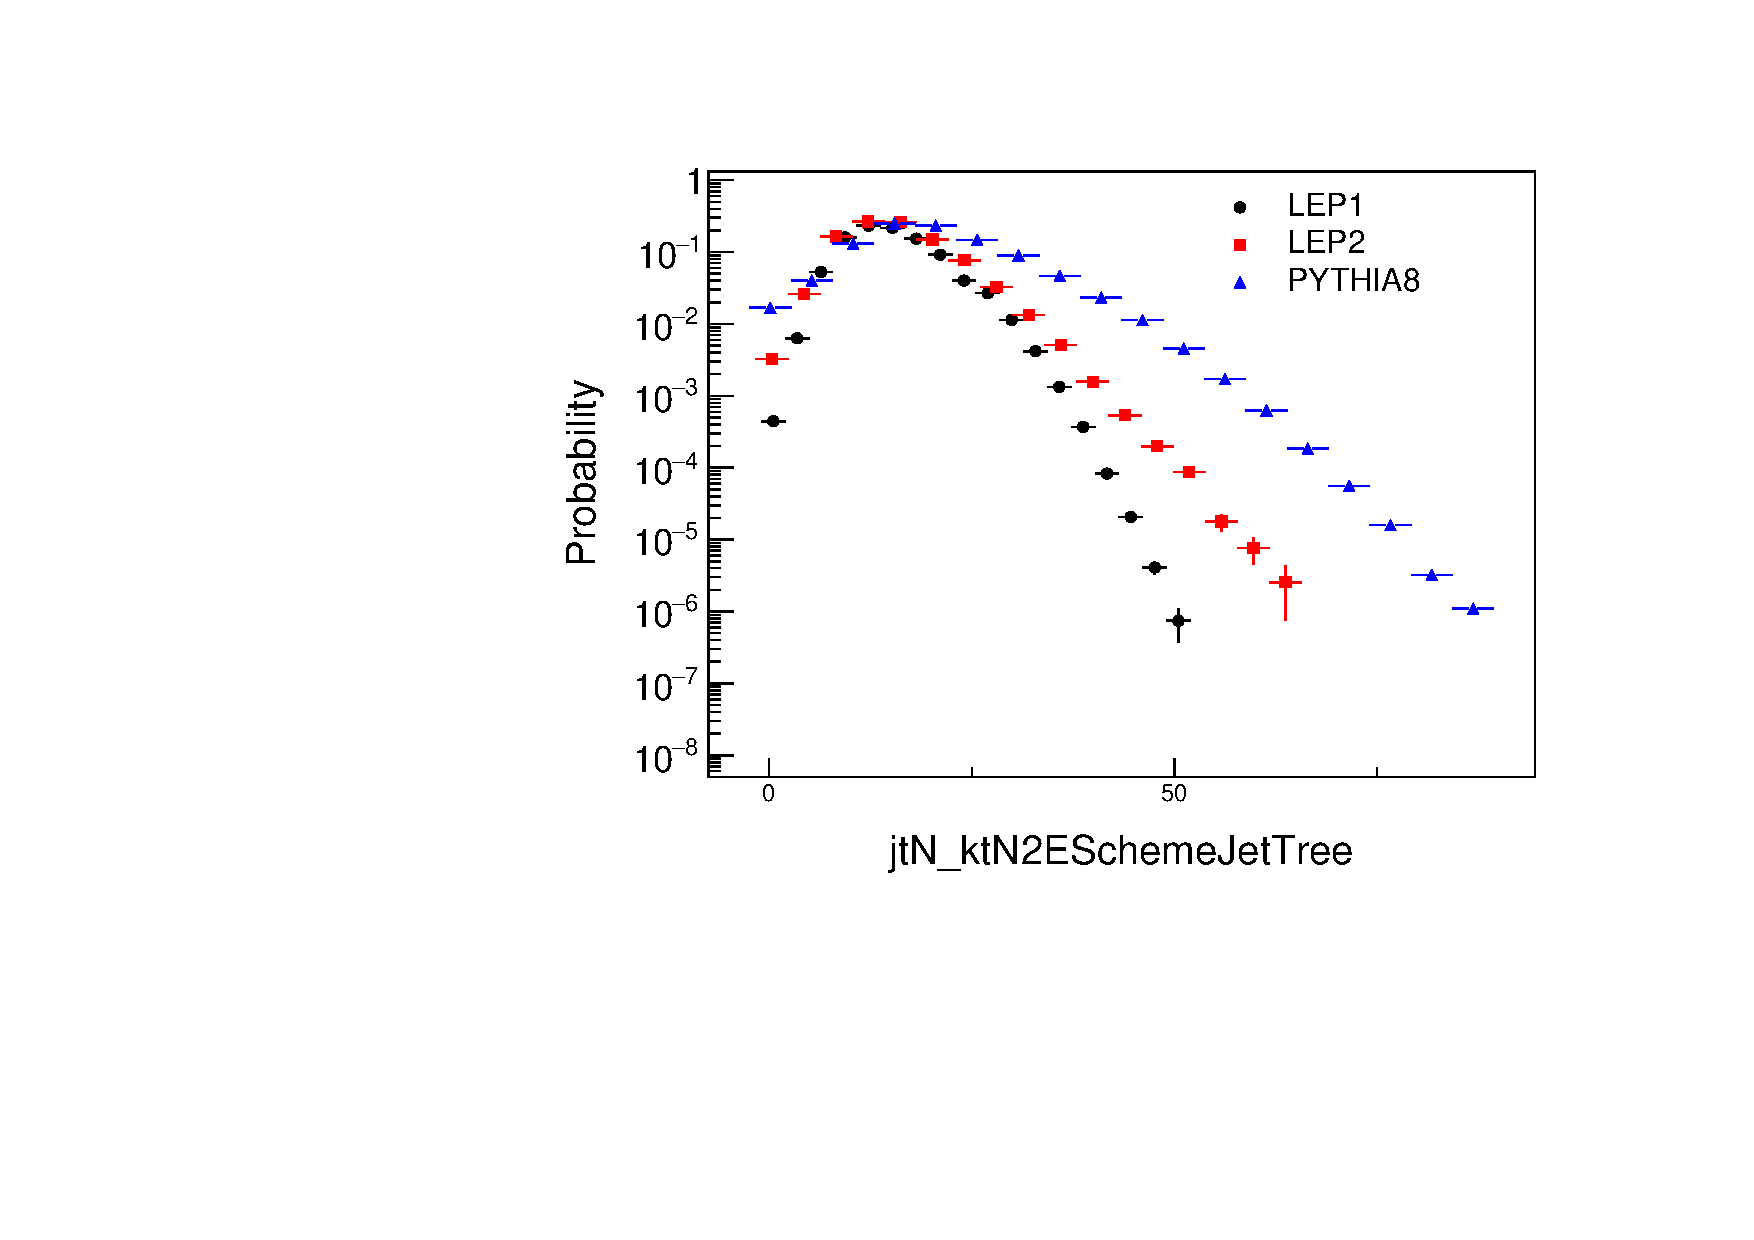
\includegraphics[width=.25\textwidth]{images/DQC/LEP1MC/jtN_ktN2ESchemeJetTree.pdf}}\hfill
\subfloat{\label{sfig:f}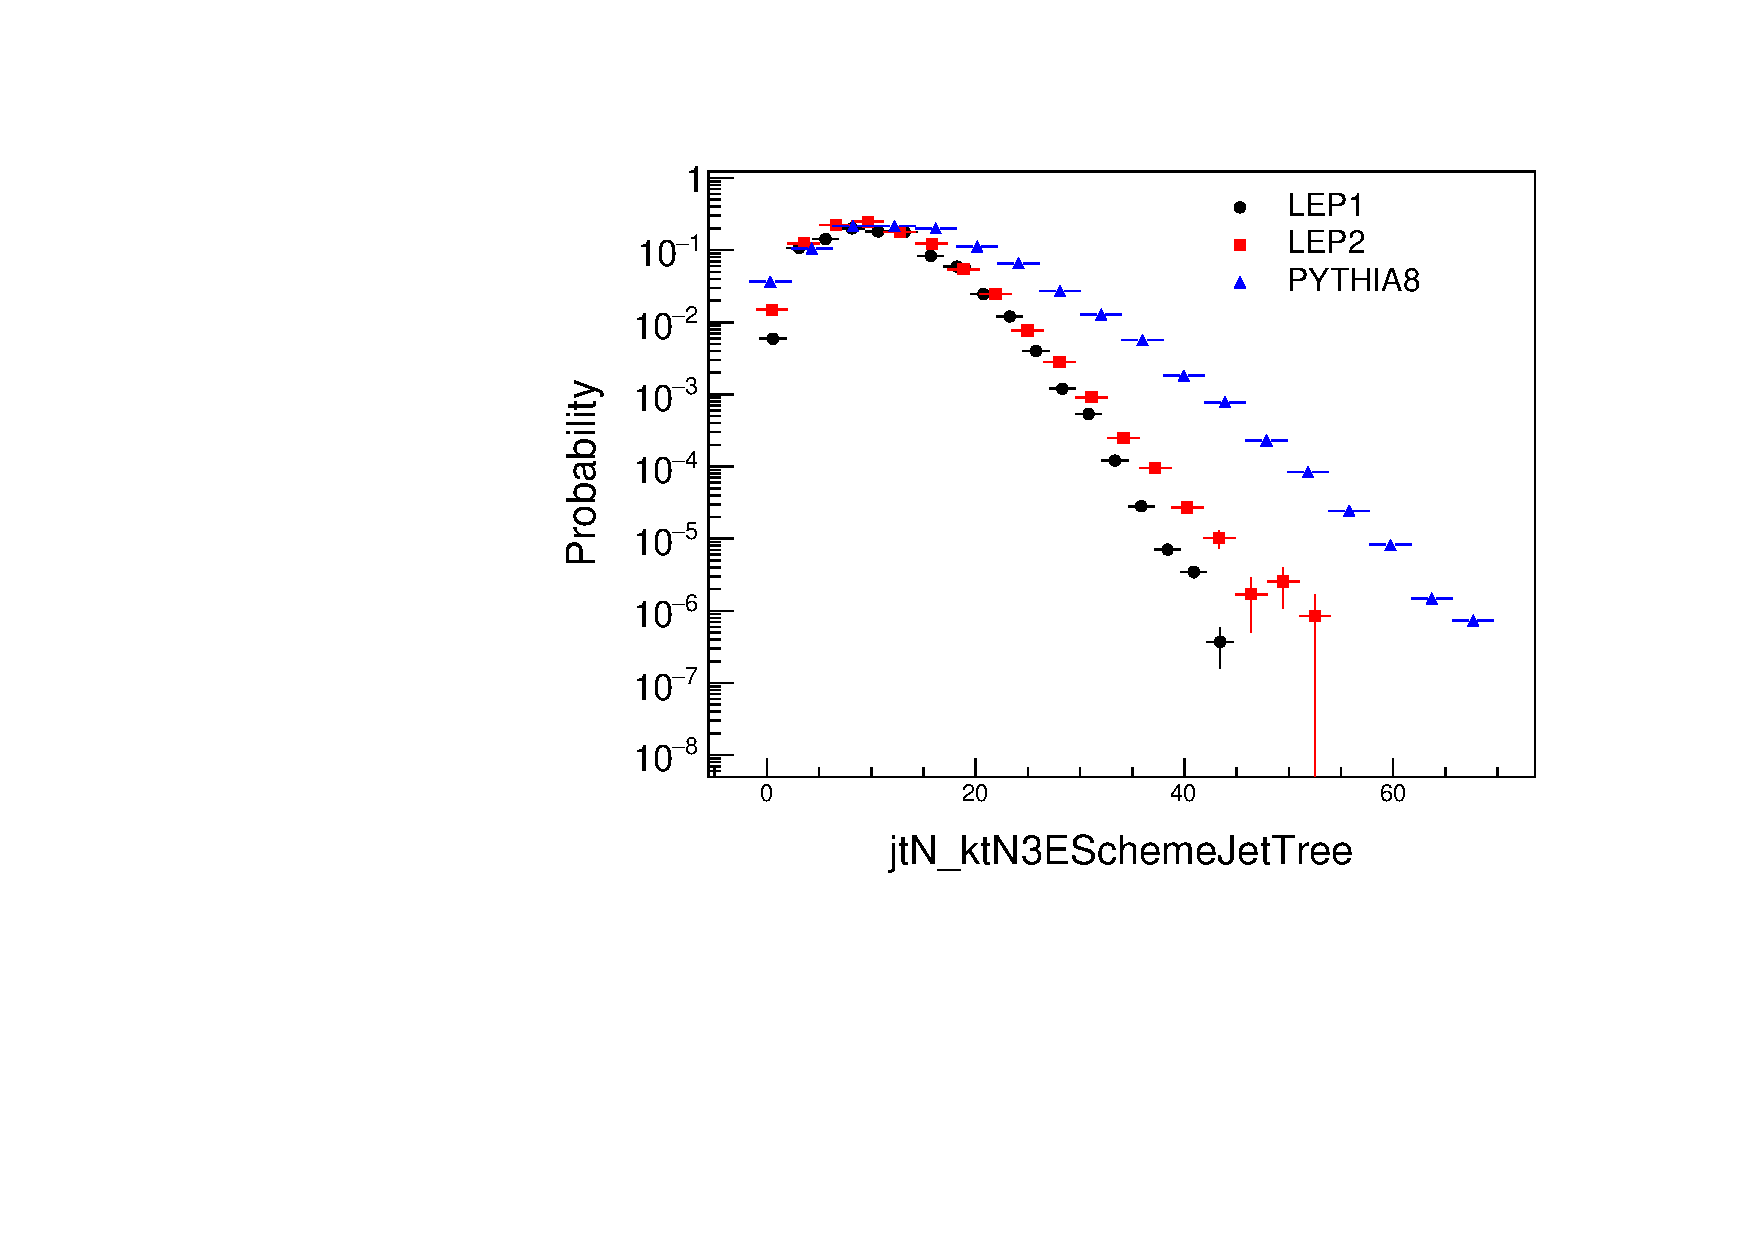
\includegraphics[width=.25\textwidth]{images/DQC/LEP1MC/jtN_ktN3ESchemeJetTree.pdf}}\hfill
\subfloat{\label{sfig:g}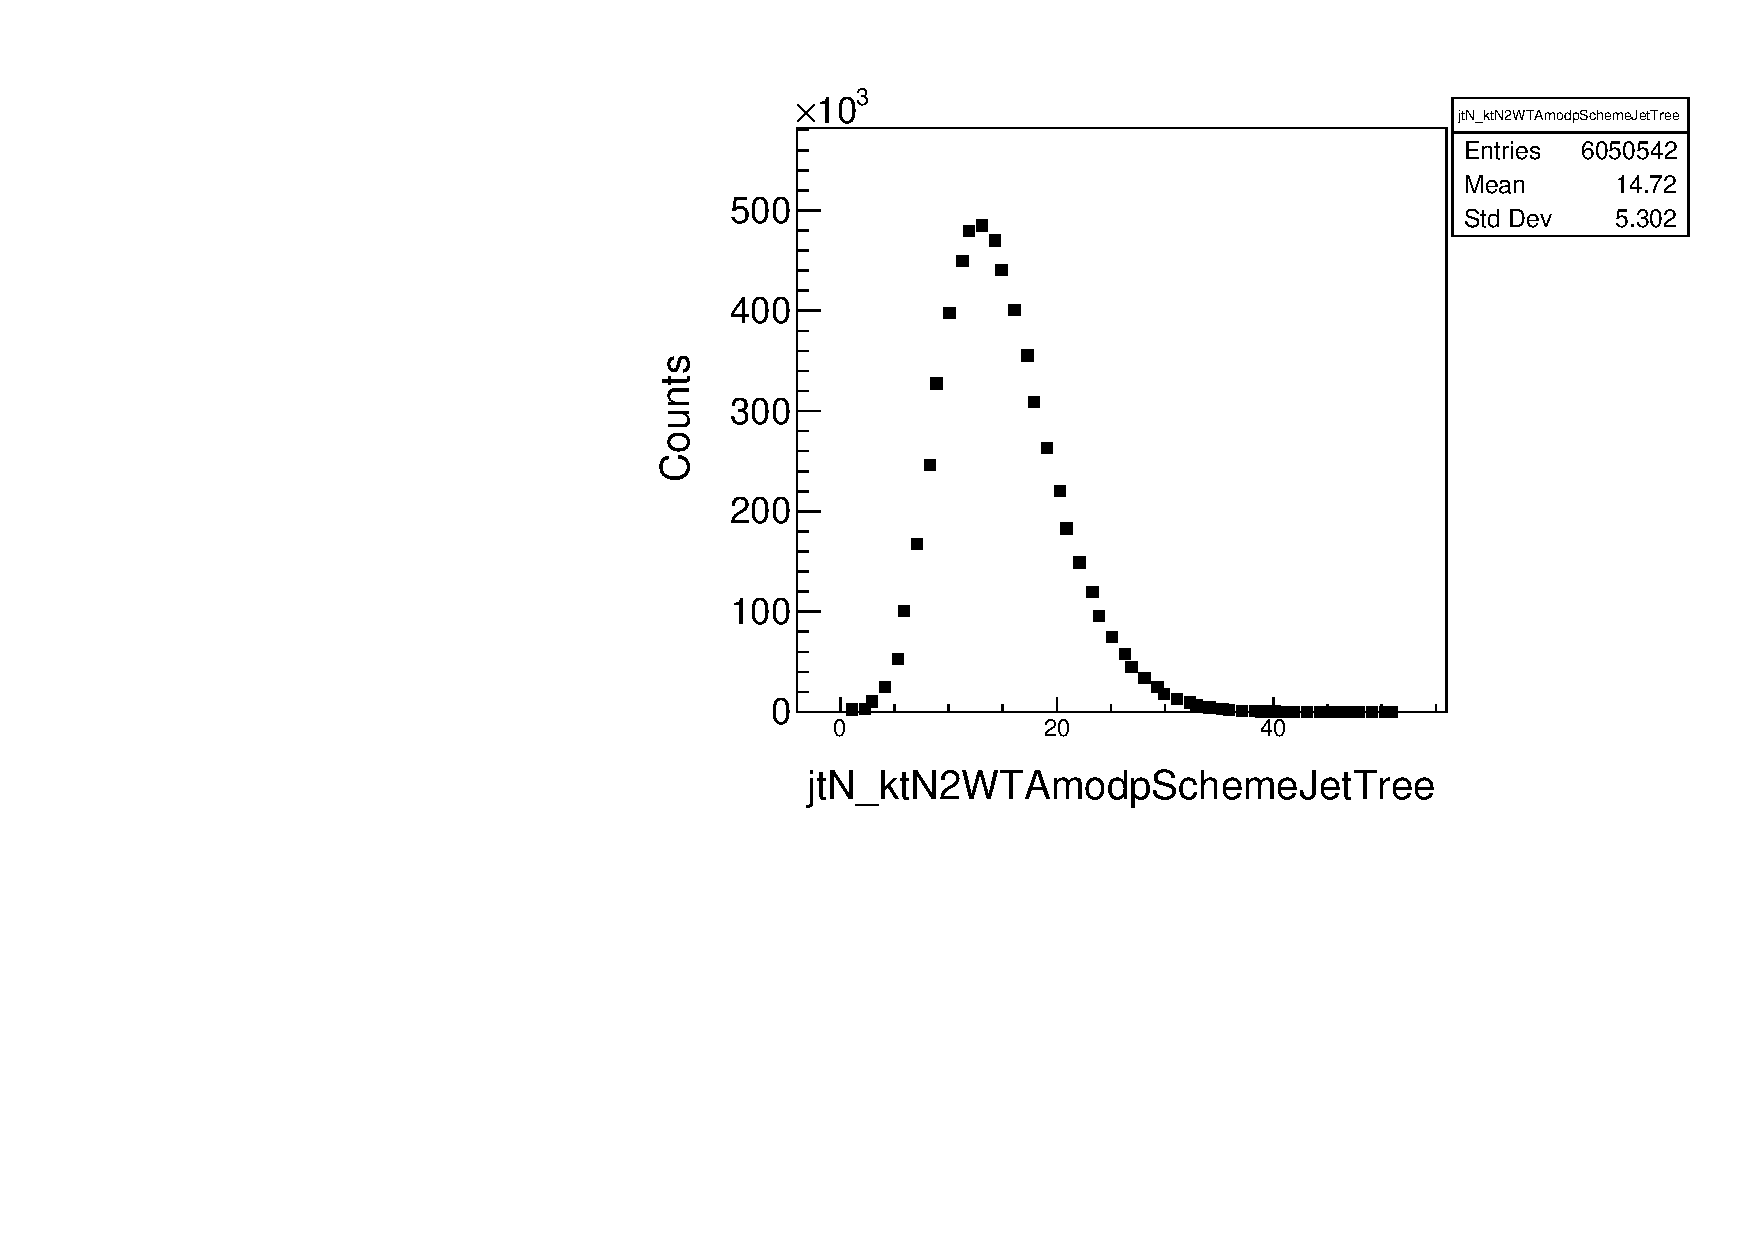
\includegraphics[width=.25\textwidth]{images/DQC/LEP1MC/jtN_ktN2WTAmodpSchemeJetTree.pdf}}\hfill
\subfloat{\label{sfig:h}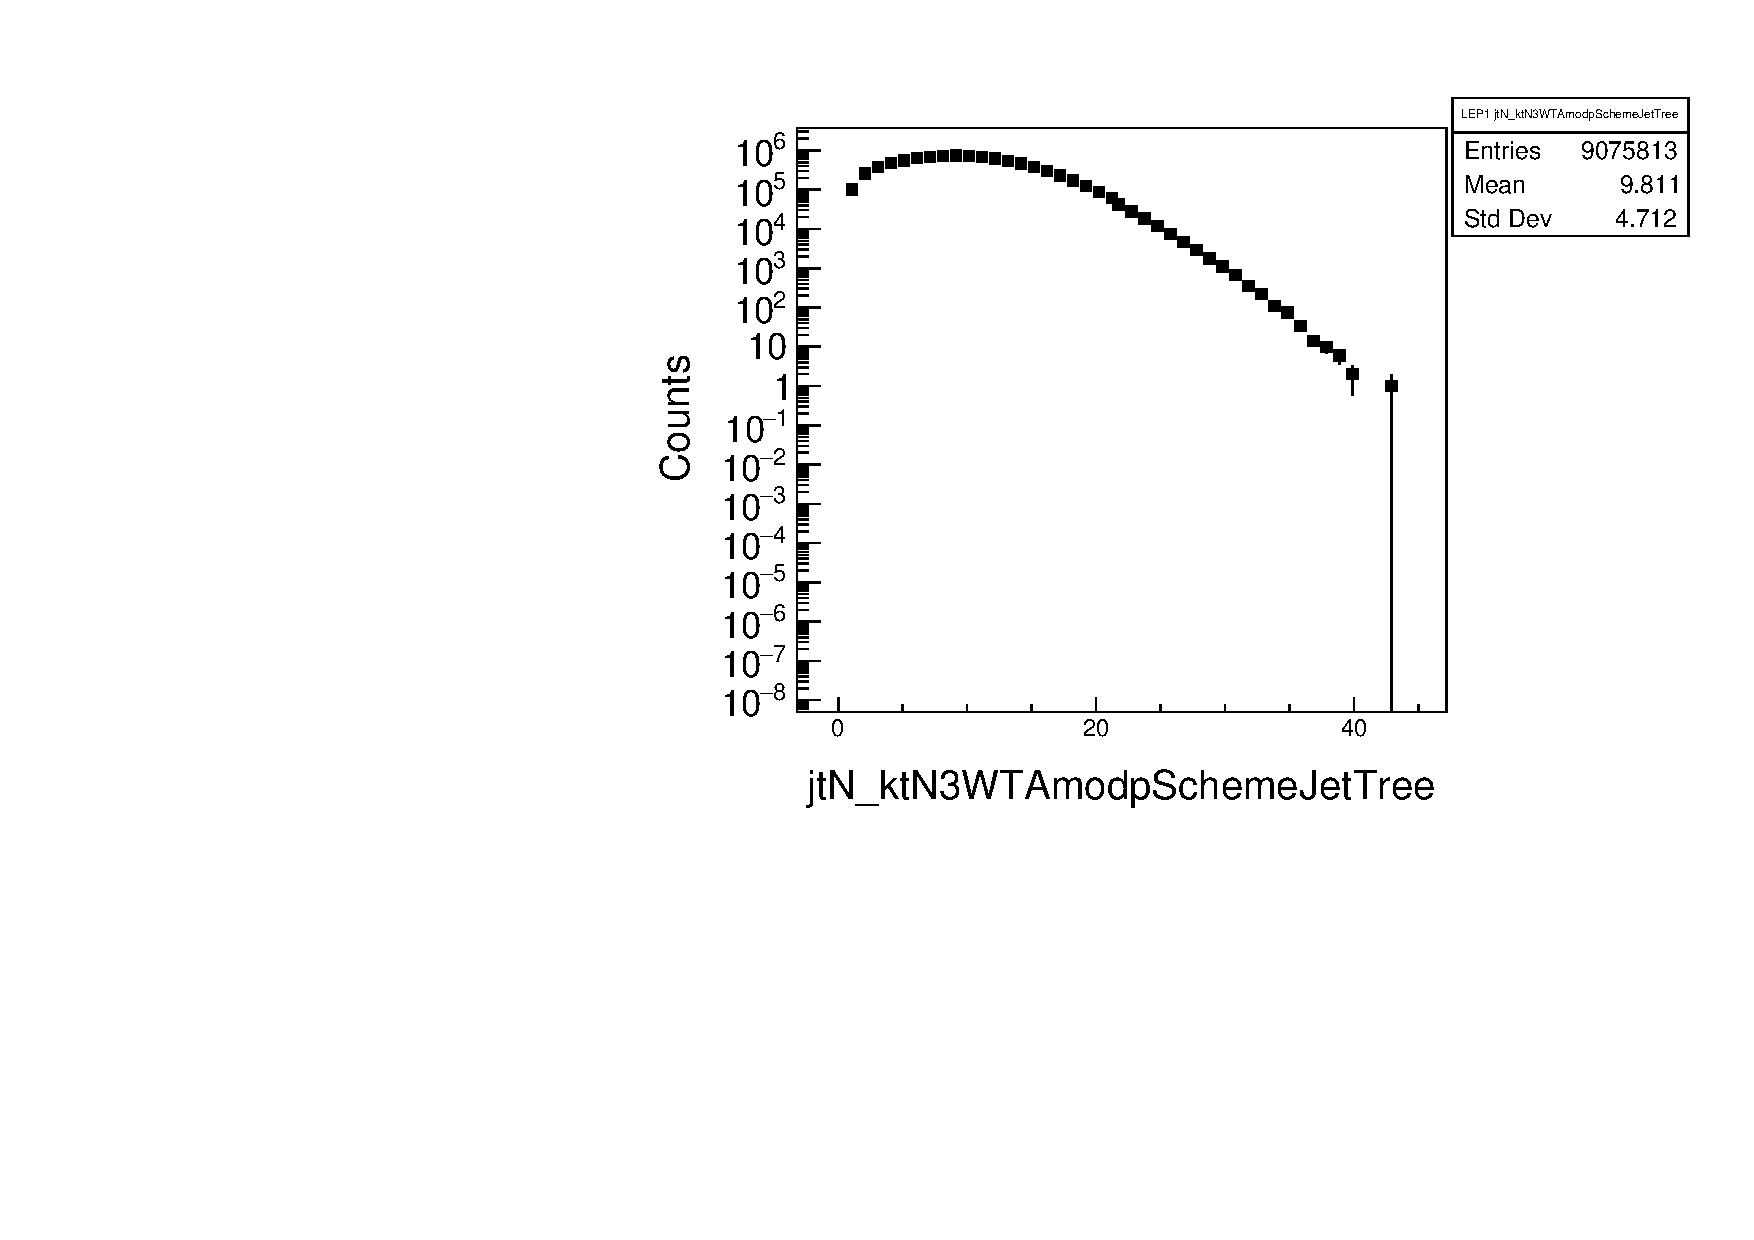
\includegraphics[width=.25\textwidth]{images/DQC/LEP1MC/jtN_ktN3WTAmodpSchemeJetTree.pdf}}\hfill
\caption{LEP1 vs LEP1 MC Jet $N$ distributions. Top row: anti-$k_t$, left to right: $R=0.4$, $E$ scheme; $R=0.8$, $E$ scheme; $R=0.4$, WTA mod p scheme; $R=0.8$, WTA mod p scheme. Bottom row: $k_t$, left to right: $N=2$, $E$ scheme; $N=3$, $E$ scheme; $N=2$, WTA mod p scheme; $N=3$; WTA mod p scheme.}  
\end{figure} 

\begin{figure}[H]
\centering
\subfloat{\label{sfig:a}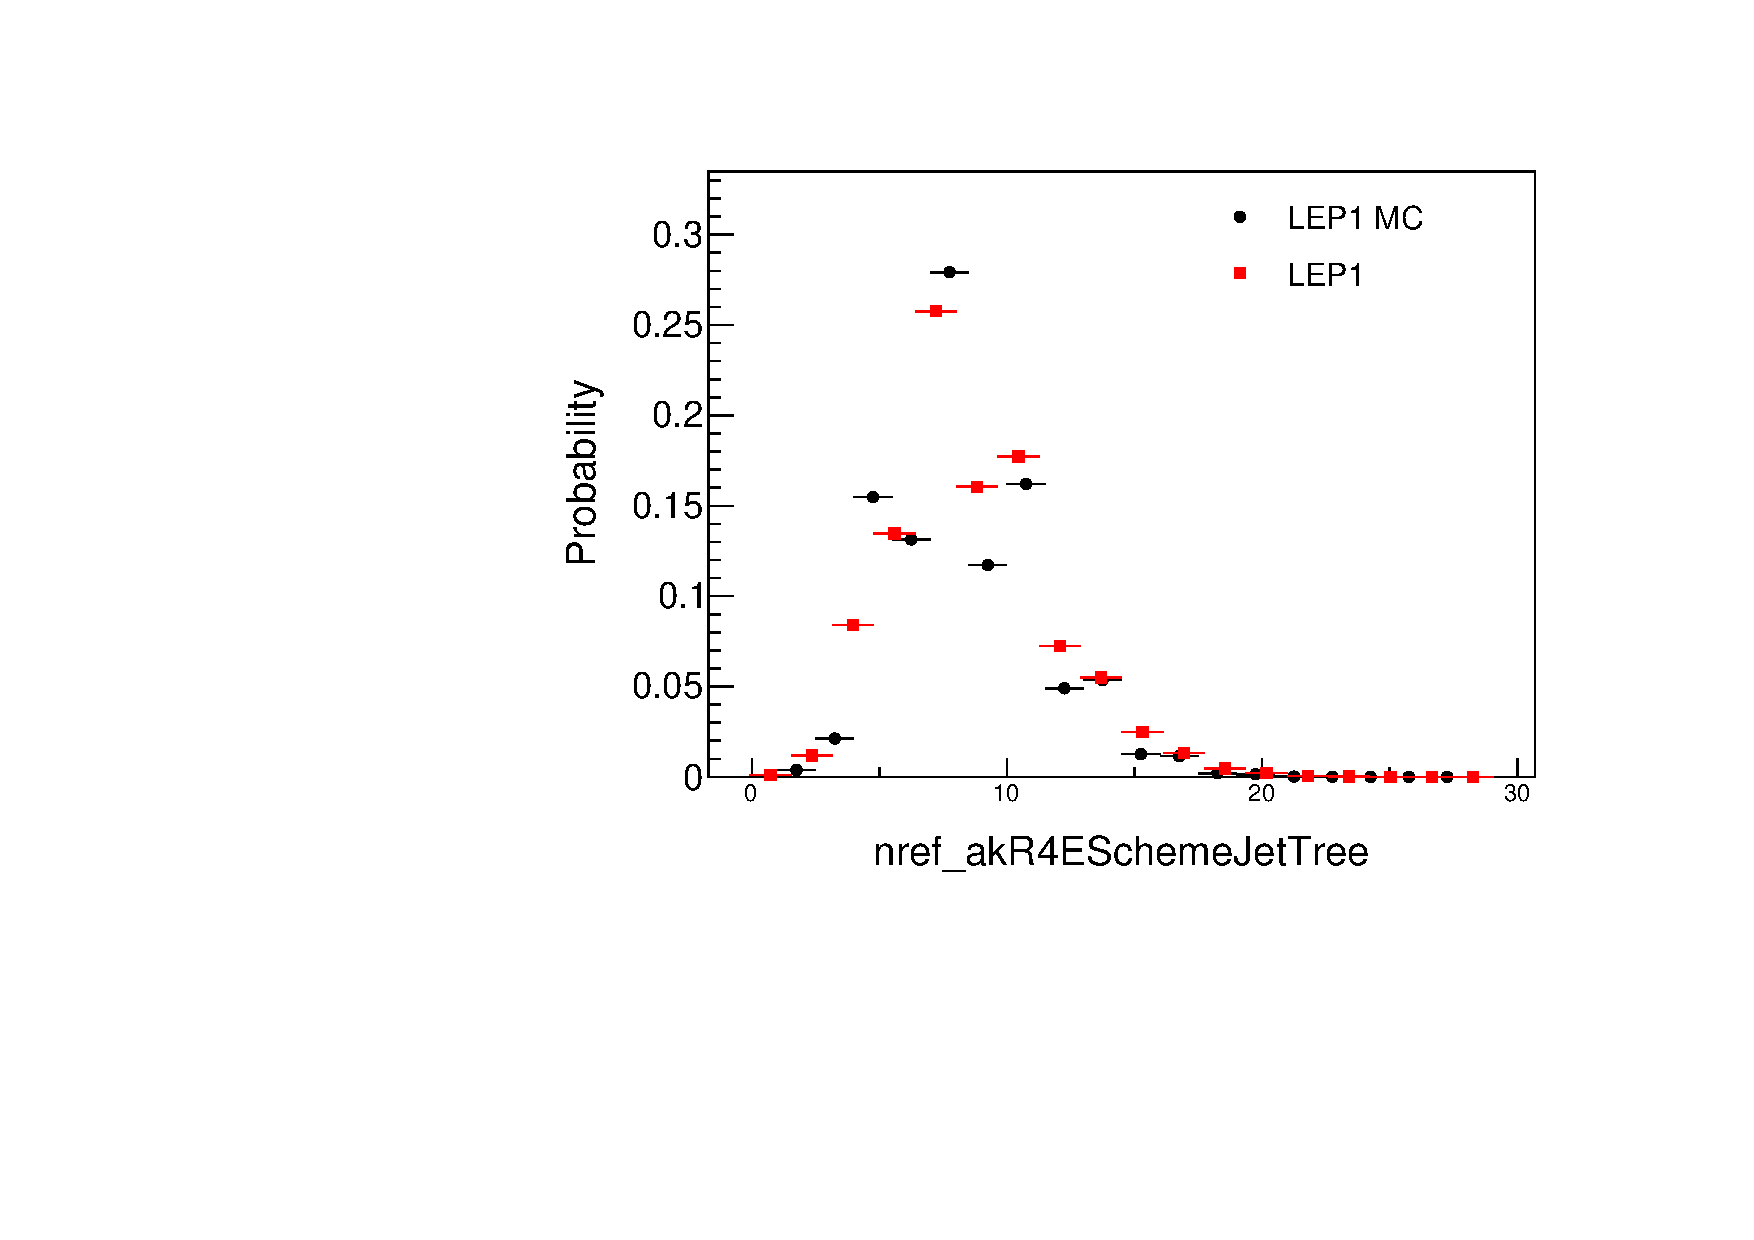
\includegraphics[width=.25\textwidth]{images/DQC/LEP1MC/nref_akR4ESchemeJetTree.pdf}}\hfill
\subfloat{\label{sfig:b}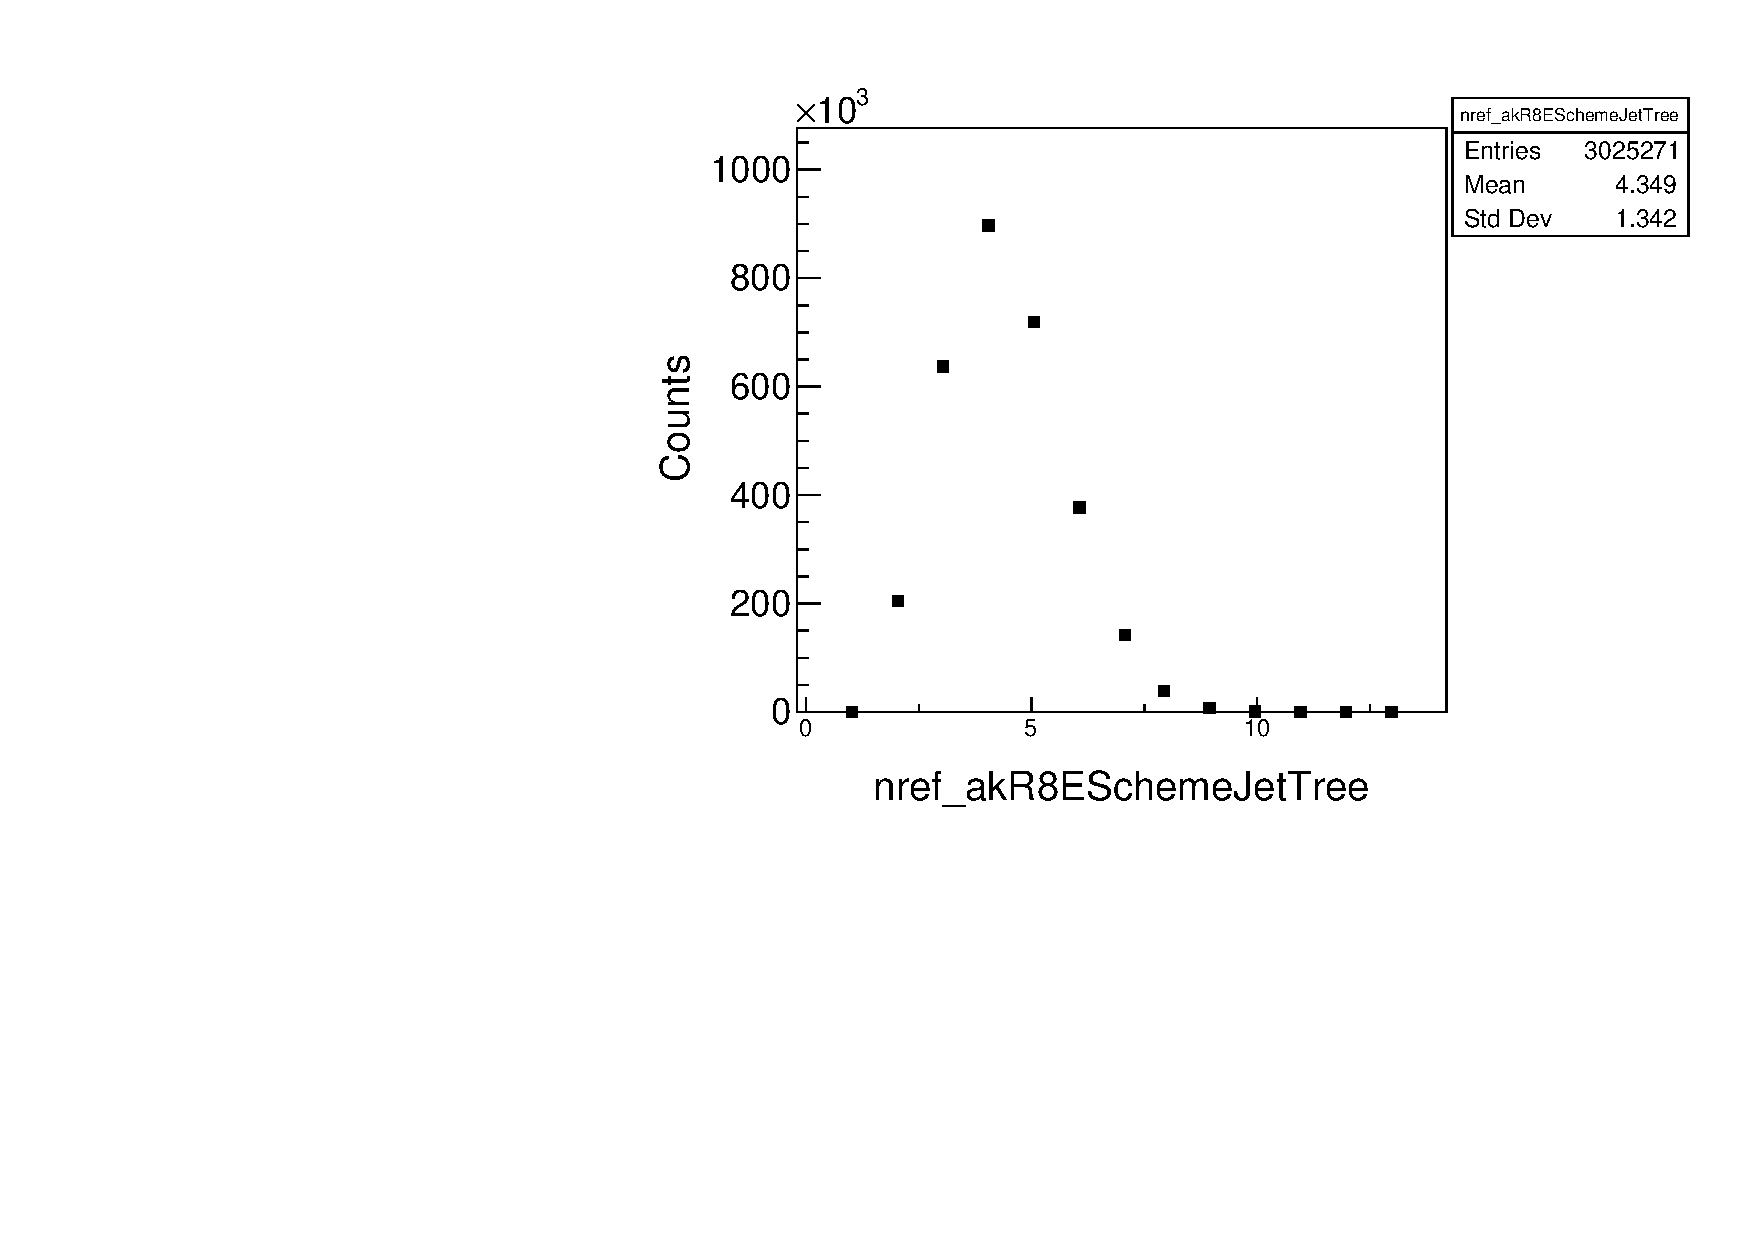
\includegraphics[width=.25\textwidth]{images/DQC/LEP1MC/nref_akR8ESchemeJetTree.pdf}}\hfill
\subfloat{\label{sfig:c}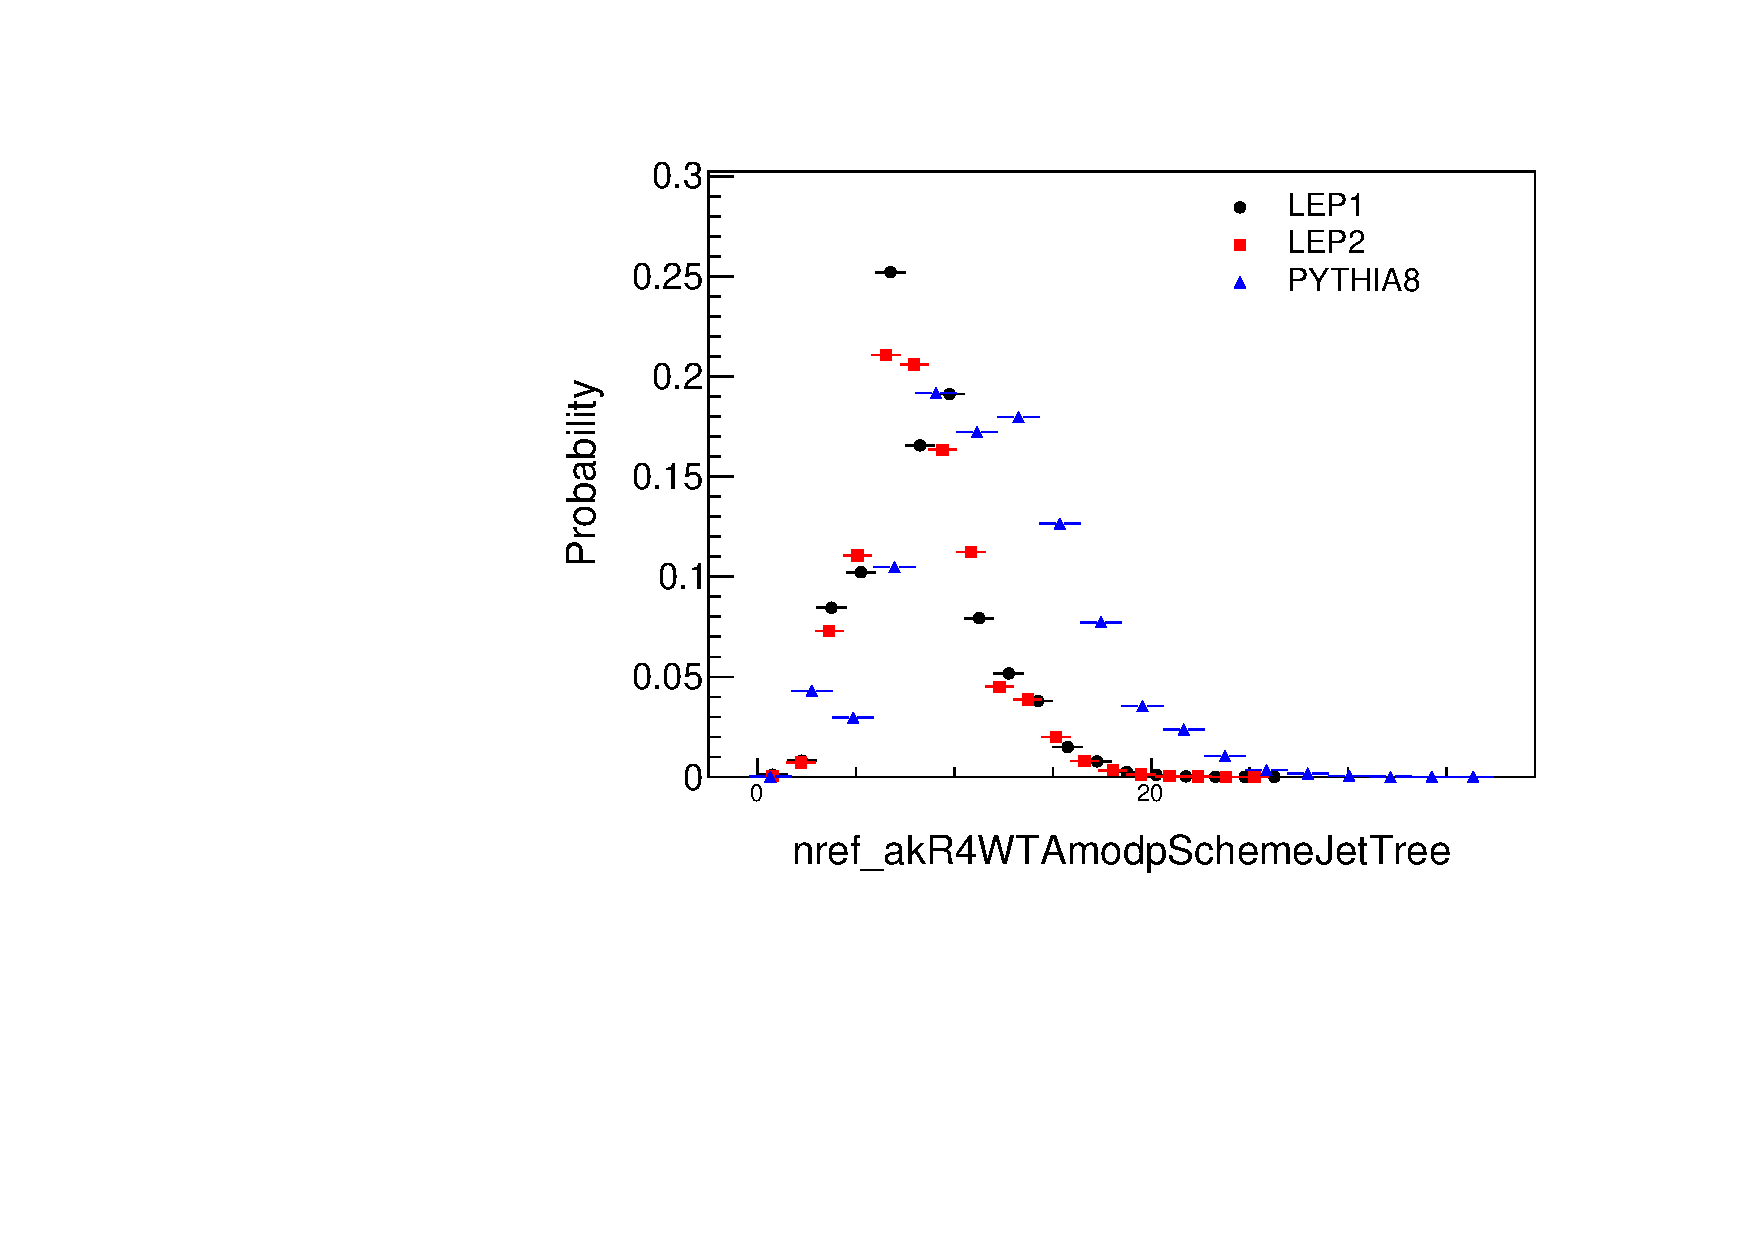
\includegraphics[width=.25\textwidth]{images/DQC/LEP1MC/nref_akR4WTAmodpSchemeJetTree.pdf}}\hfill
\subfloat{\label{sfig:d}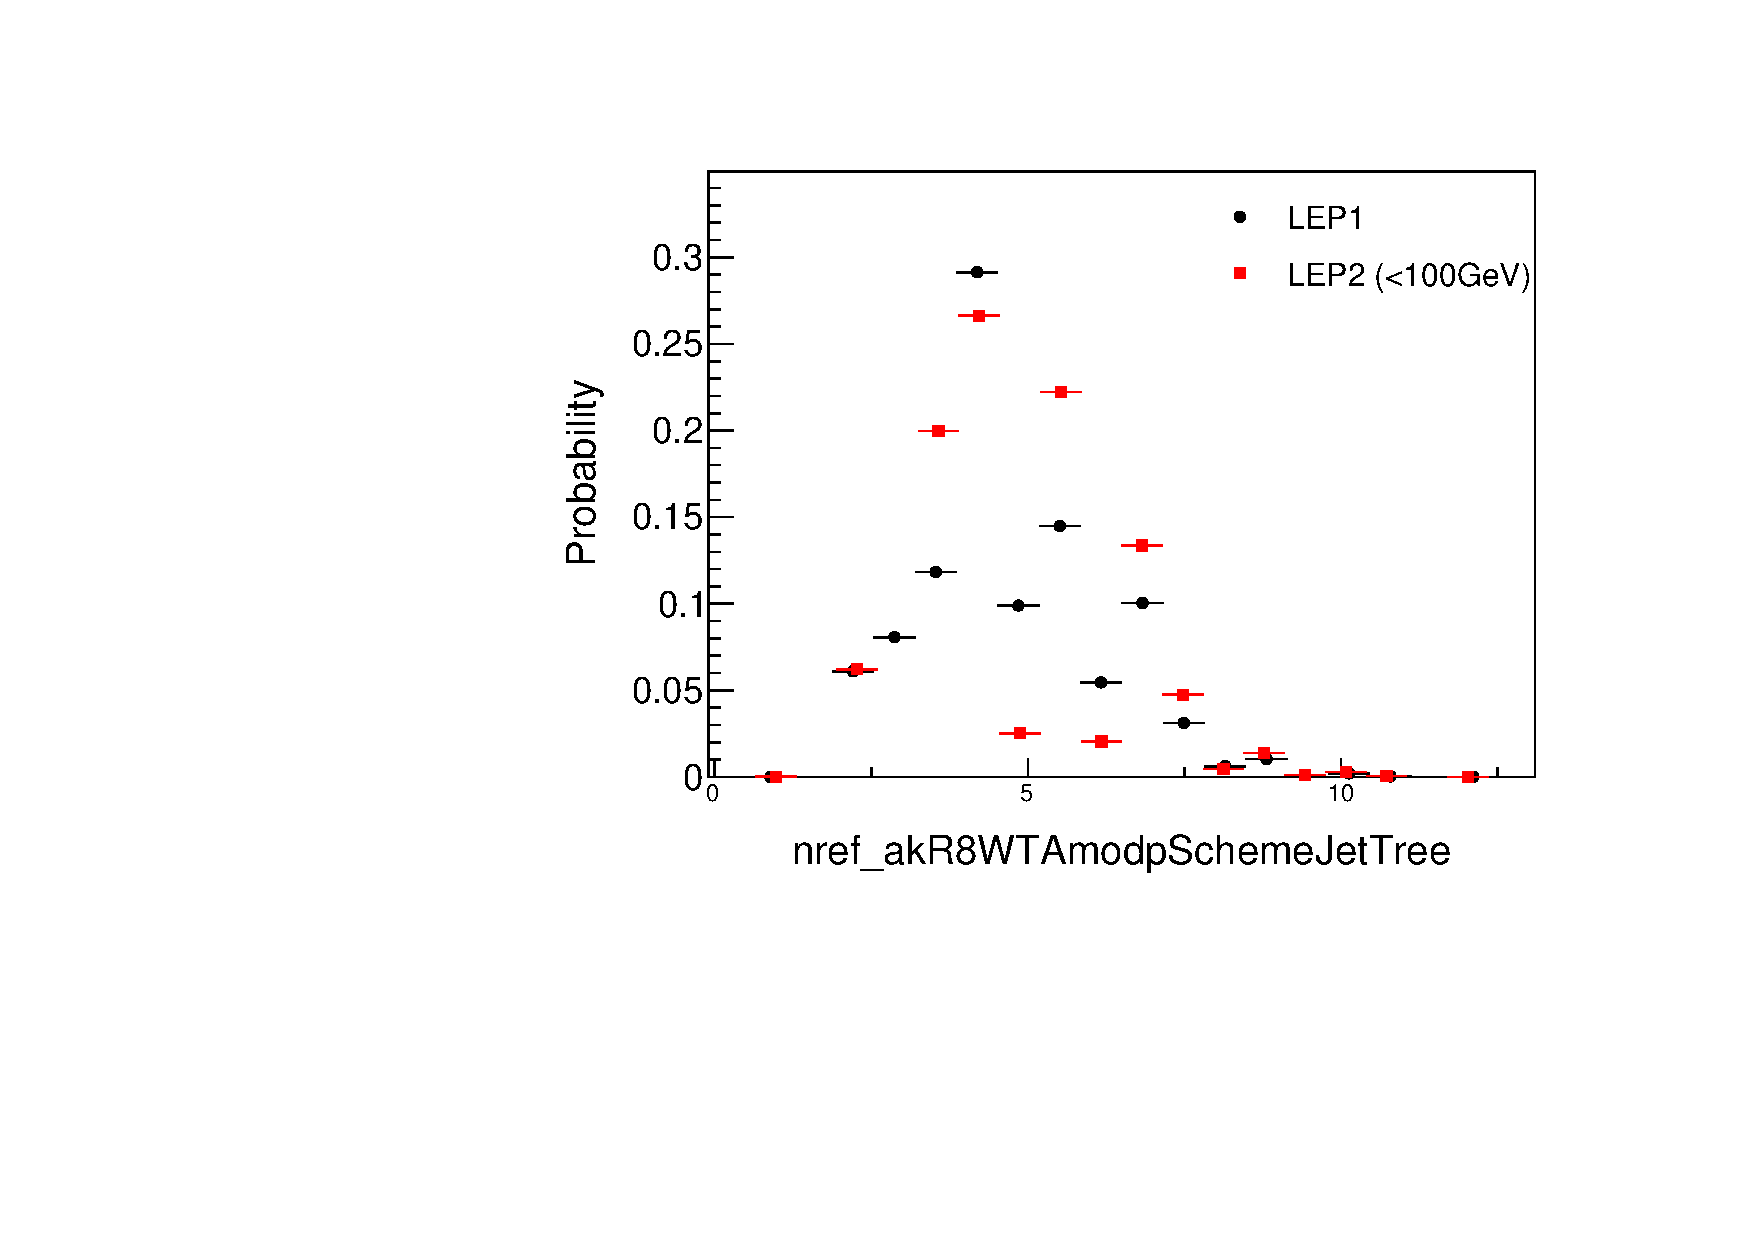
\includegraphics[width=.25\textwidth]{images/DQC/LEP1MC/nref_akR8WTAmodpSchemeJetTree.pdf}}\hfill %row end
\subfloat{\label{sfig:e}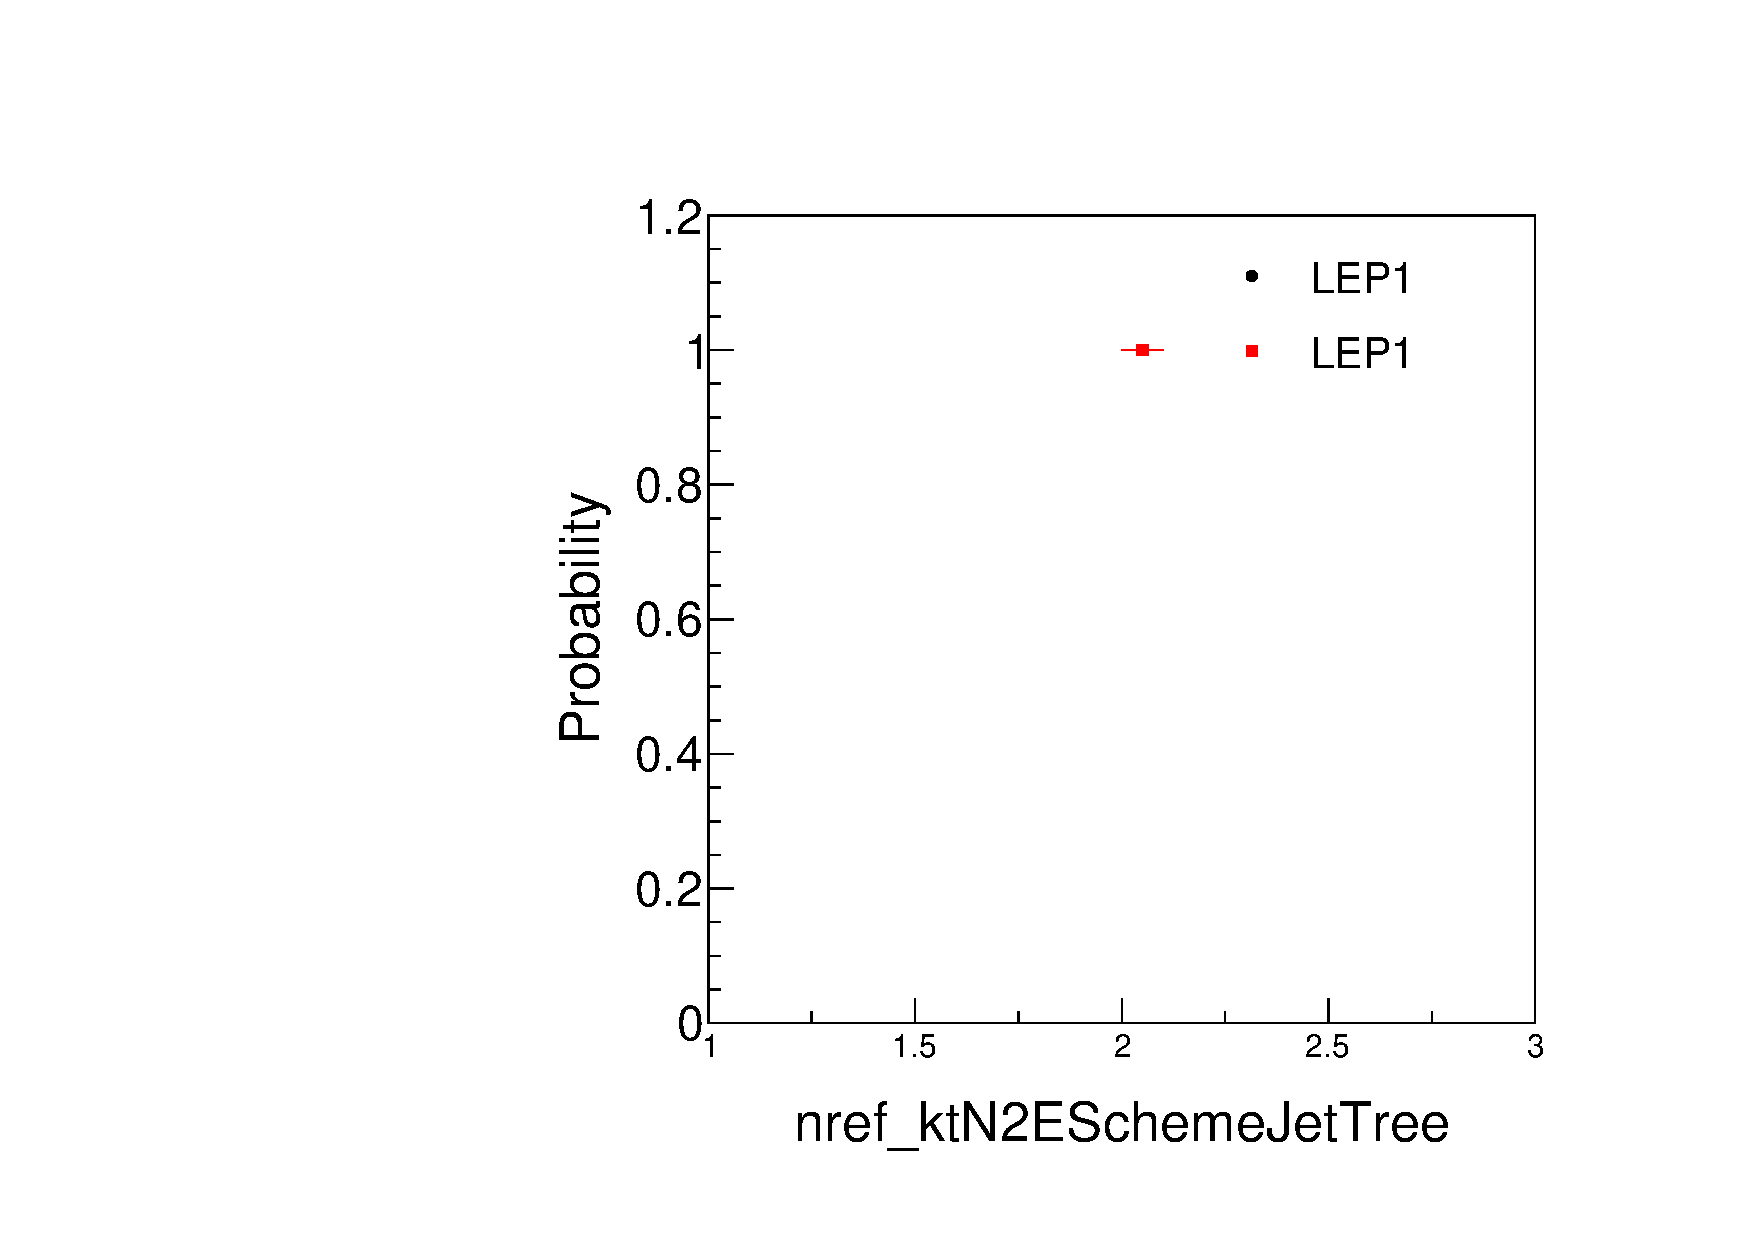
\includegraphics[width=.25\textwidth]{images/DQC/LEP1MC/nref_ktN2ESchemeJetTree.pdf}}\hfill
\subfloat{\label{sfig:f}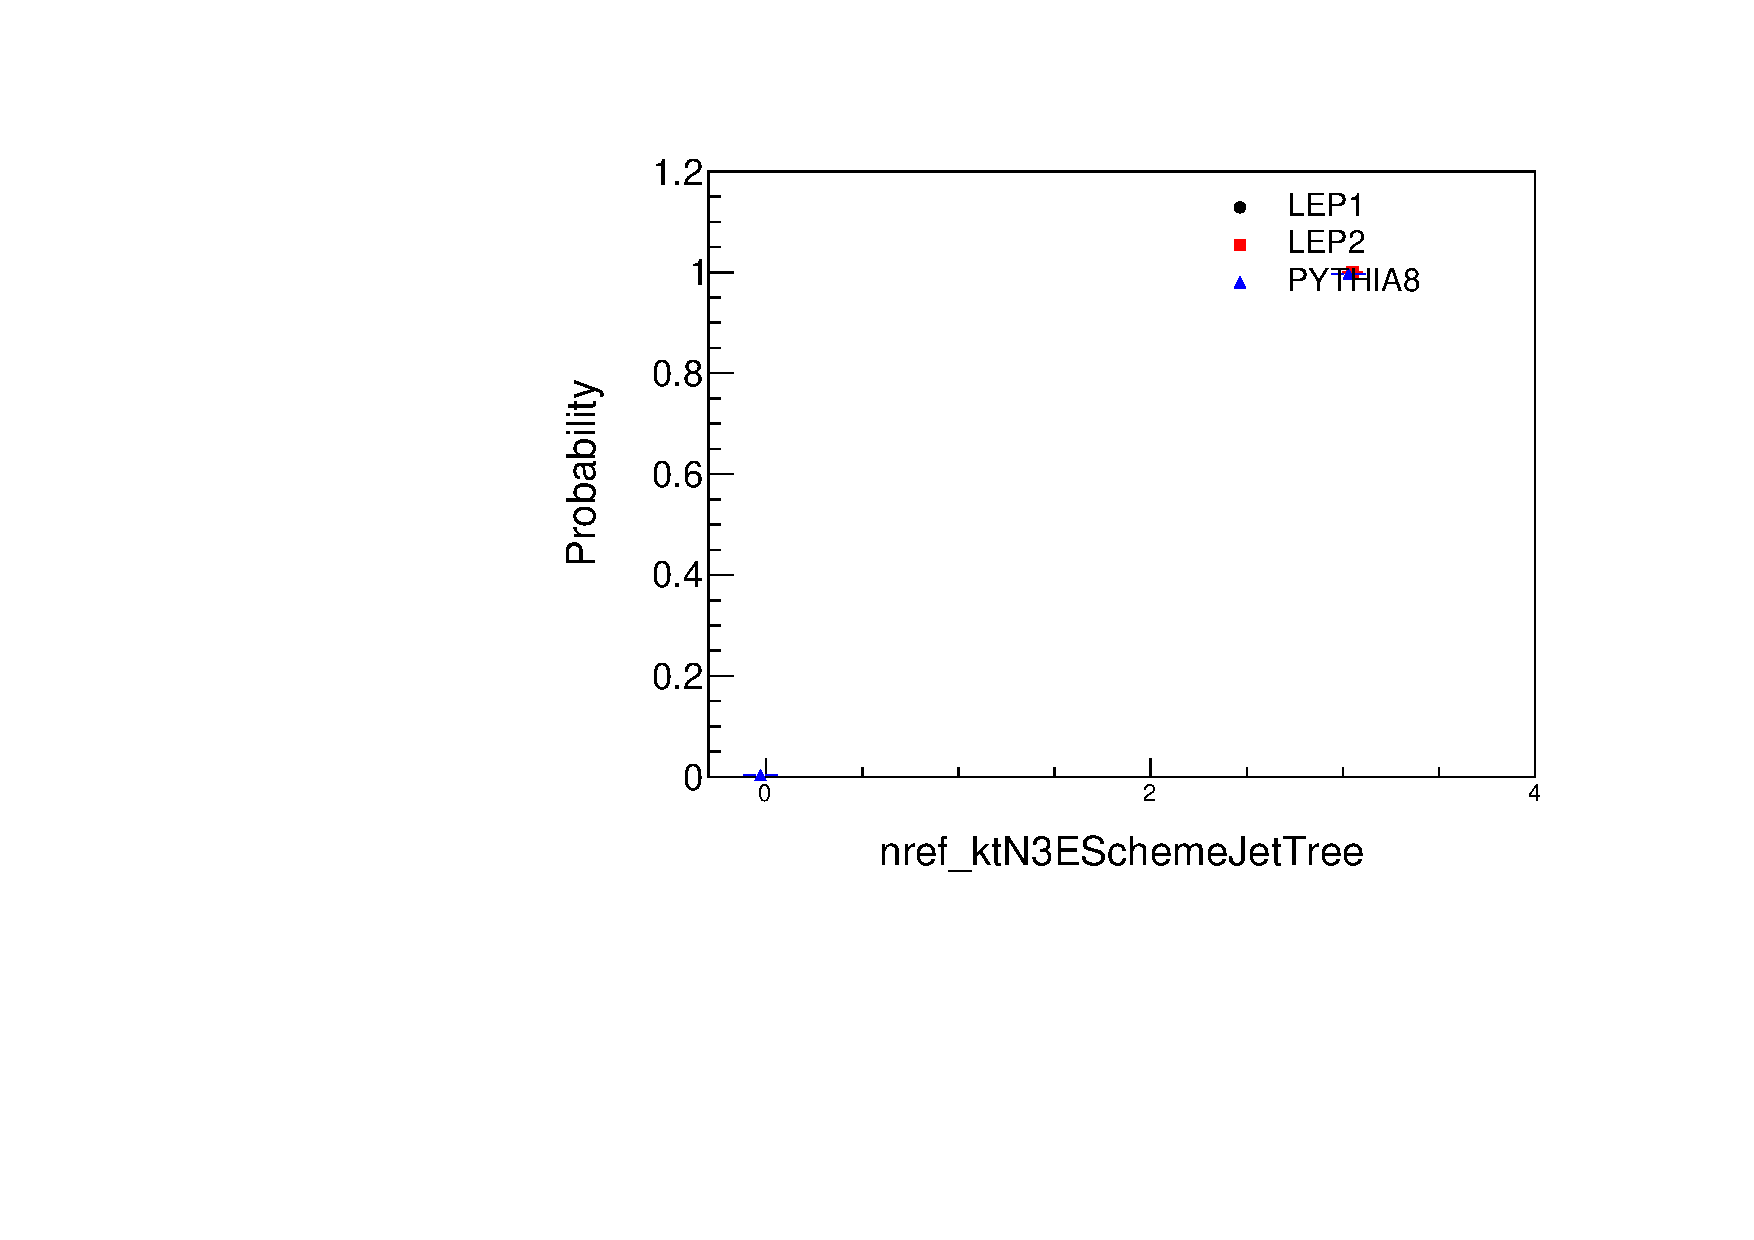
\includegraphics[width=.25\textwidth]{images/DQC/LEP1MC/nref_ktN3ESchemeJetTree.pdf}}\hfill
\subfloat{\label{sfig:g}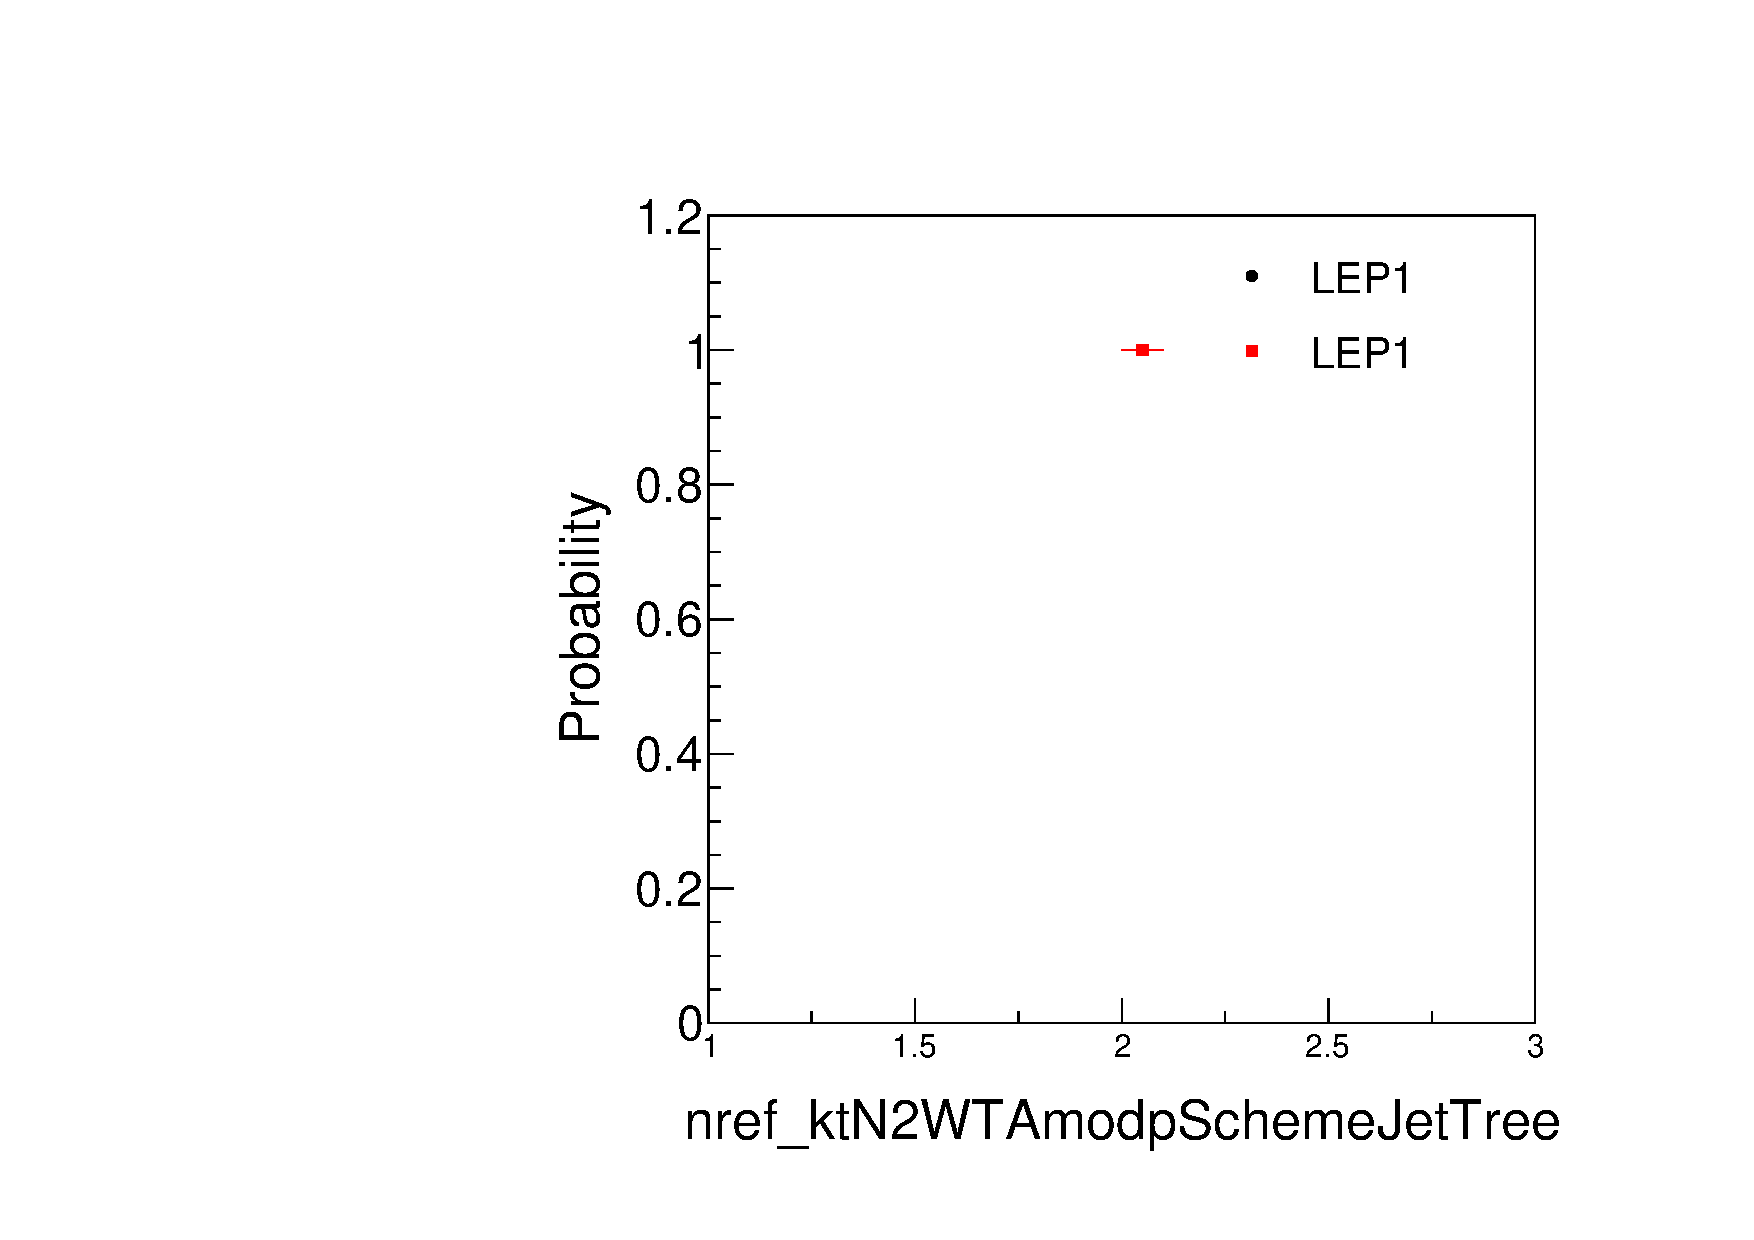
\includegraphics[width=.25\textwidth]{images/DQC/LEP1MC/nref_ktN2WTAmodpSchemeJetTree.pdf}}\hfill
\subfloat{\label{sfig:h}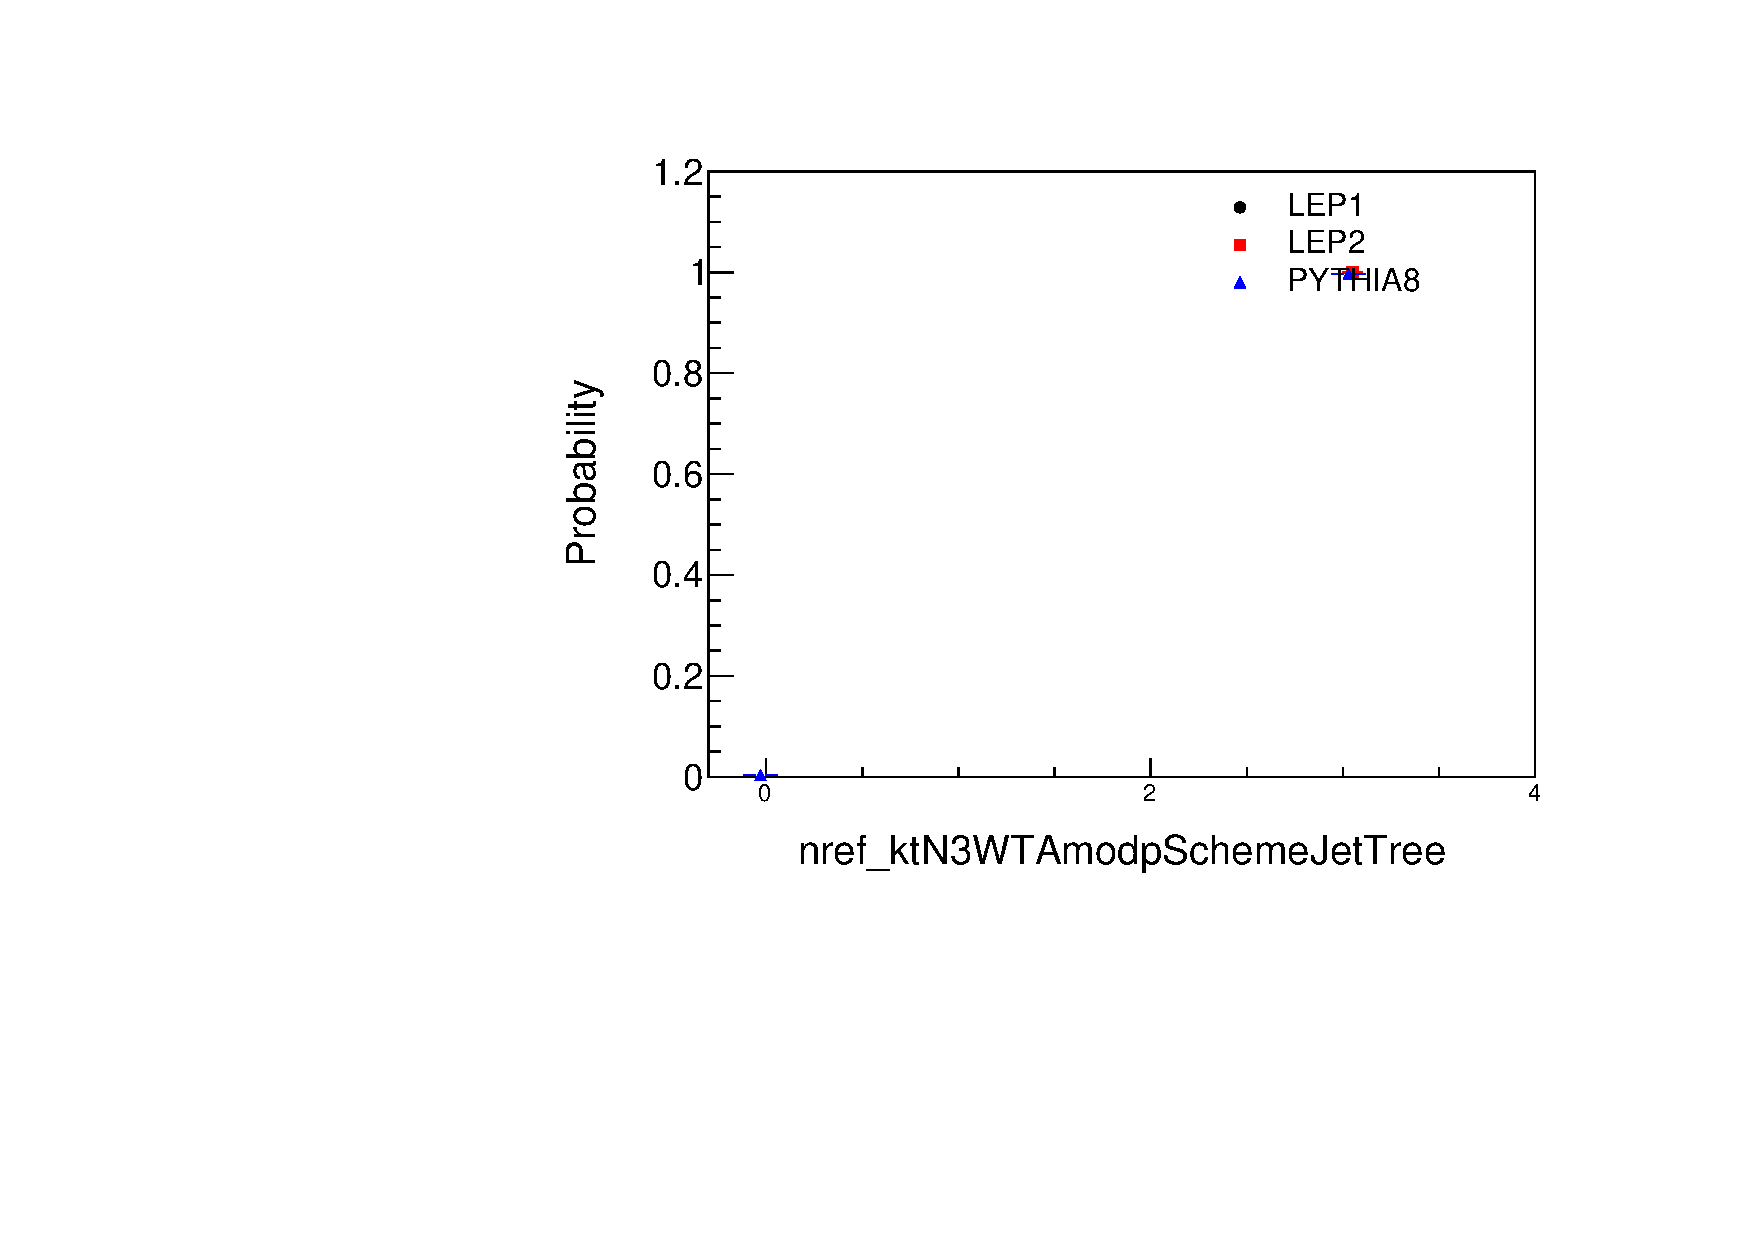
\includegraphics[width=.25\textwidth]{images/DQC/LEP1MC/nref_ktN3WTAmodpSchemeJetTree.pdf}}\hfill
\caption{LEP1 vs LEP1 MC Jet nref distributions. Top row: anti-$k_t$, left to right: $R=0.4$, $E$ scheme; $R=0.8$, $E$ scheme; $R=0.4$, WTA mod p scheme; $R=0.8$, WTA mod p scheme. Bottom row: $k_t$, left to right: $N=2$, $E$ scheme; $N=3$, $E$ scheme; $N=2$, WTA mod p scheme; $N=3$; WTA mod p scheme.}  
\end{figure}

\begin{figure}[H]
\centering
\subfloat{\label{sfig:a}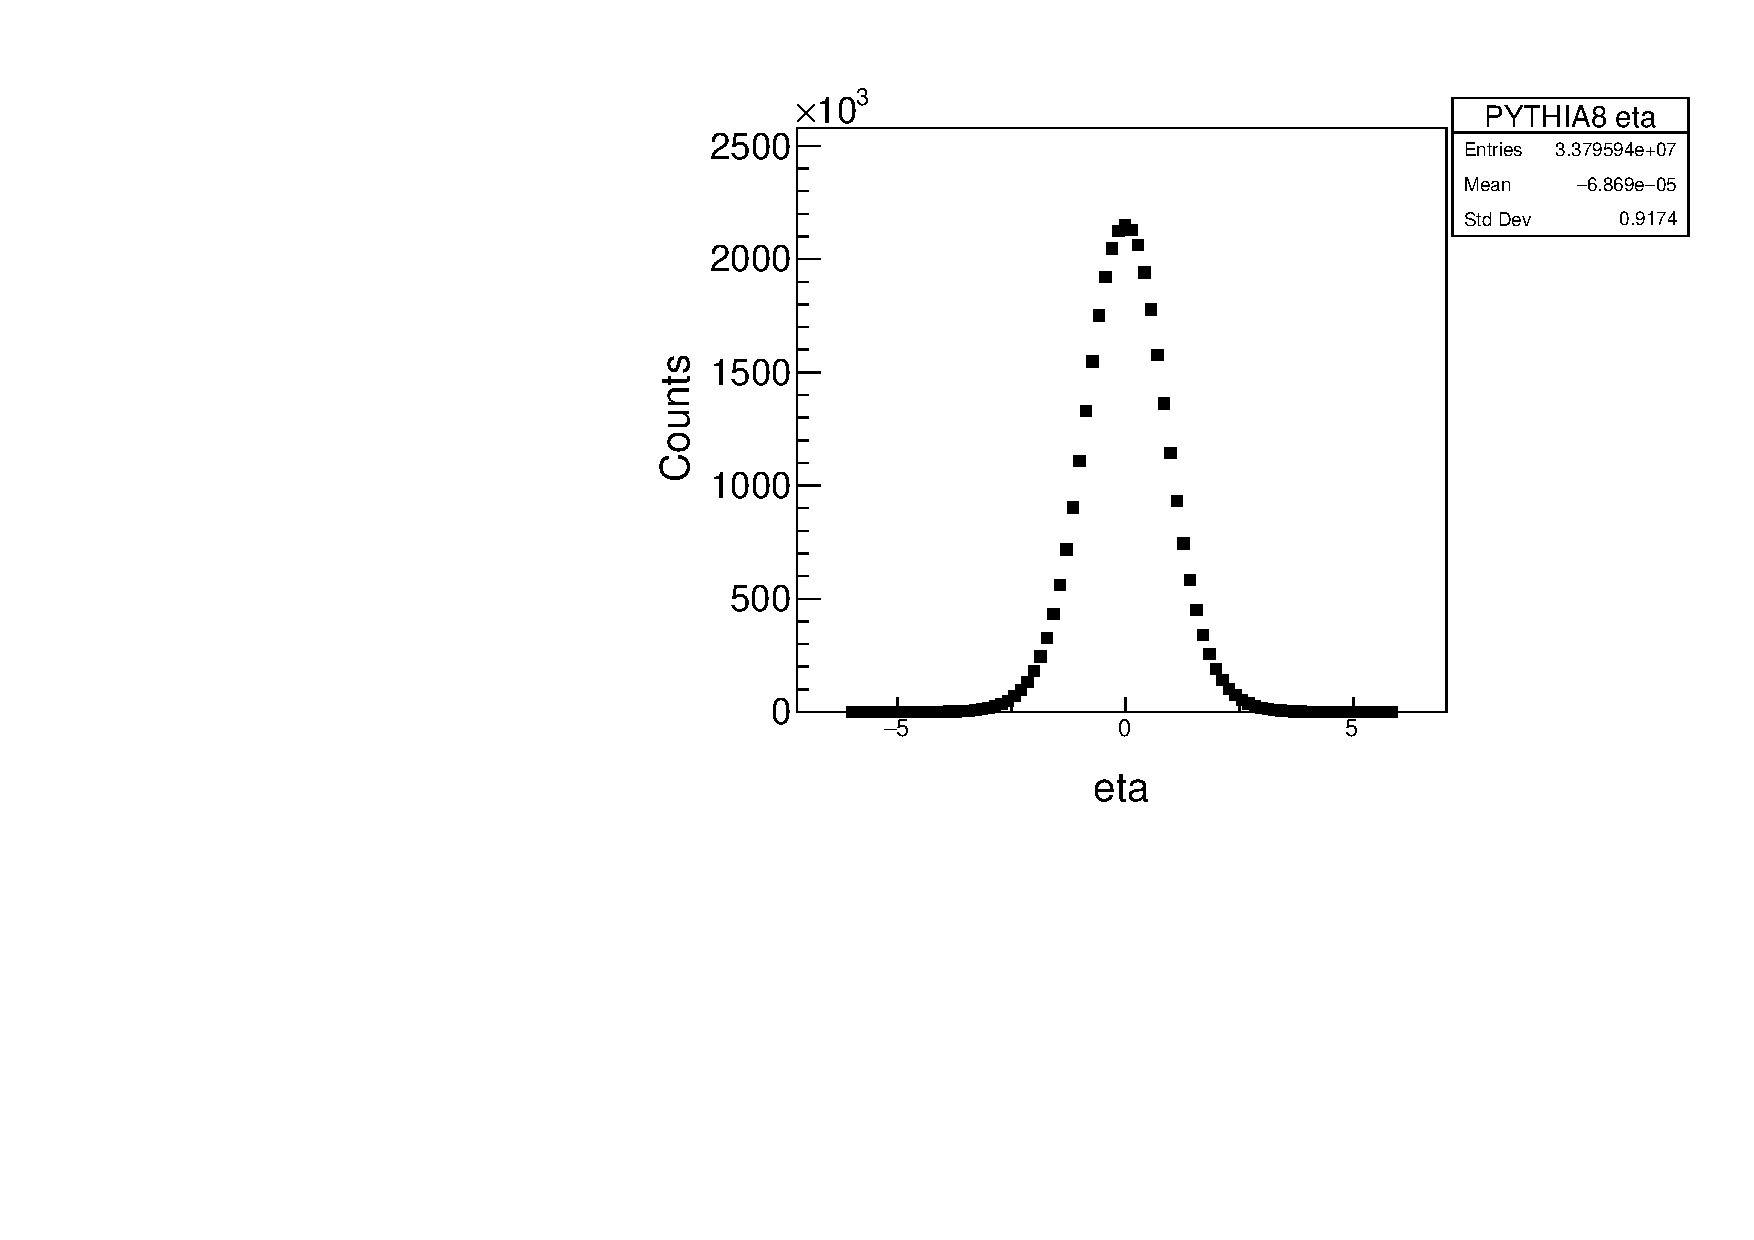
\includegraphics[width=.33\textwidth]{images/DQC/LEP1MC/eta.pdf}}\hfill
\subfloat{\label{sfig:b}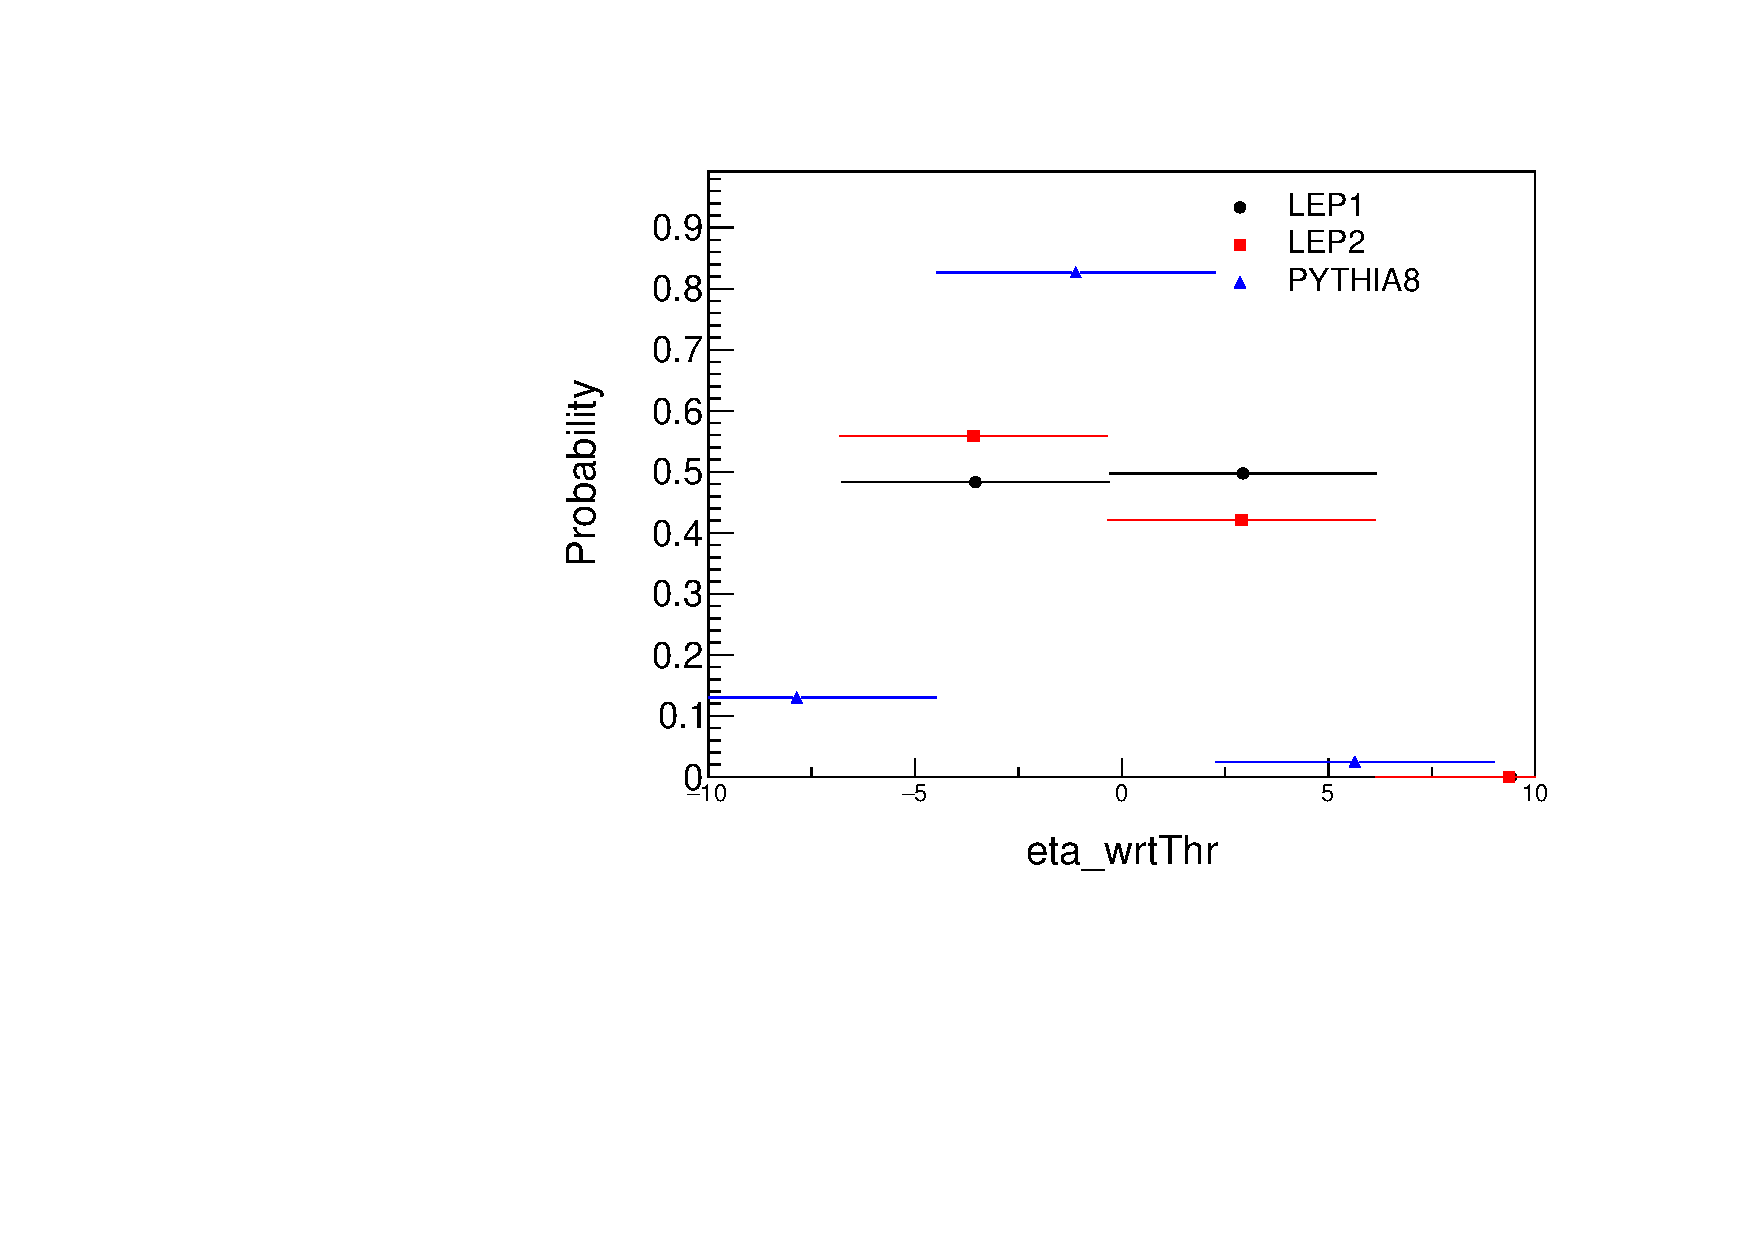
\includegraphics[width=.33\textwidth]{images/DQC/LEP1MC/eta_wrtThr.pdf}}\hfill
\subfloat{\label{sfig:c}\includegraphics[width=.33\textwidth]{images/DQC/LEP1MC/eta_wrtChThr.pdf}}\hfill
\caption{LEP1 vs LEP1 MC $\eta$ distributions. Left to right: $\eta$; $\eta$ with respect to thrust axis; $\eta$ with respect to charged thrust axis.}
\end{figure}

\begin{figure}[H]
\centering
\subfloat{\label{sfig:a}\includegraphics[width=.33\textwidth]{images/DQC/LEP1MC/phi.pdf}}\hfill
\subfloat{\label{sfig:b}\includegraphics[width=.33\textwidth]{images/DQC/LEP1MC/phi_wrtThr.pdf}}\hfill
\subfloat{\label{sfig:c}\includegraphics[width=.33\textwidth]{images/DQC/LEP1MC/phi_wrtChThr.pdf}}\hfill
\caption{LEP1 vs LEP1 MC $\phi$ distributions. Left to right: $\phi$; $\phi$ with respect to thrust axis; $\phi$ with respect to charged thrust axis.}
\end{figure}

\begin{figure}[H]
\centering
\subfloat{\label{sfig:a}\includegraphics[width=.33\textwidth]{images/DQC/LEP1MC/pt.pdf}}\hfill
\subfloat{\label{sfig:b}\includegraphics[width=.33\textwidth]{images/DQC/LEP1MC/pt_wrtThr.pdf}}\hfill
\subfloat{\label{sfig:c}\includegraphics[width=.33\textwidth]{images/DQC/LEP1MC/pt_wrtChThr.pdf}}\hfill
\caption{LEP1 vs LEP1 MC $p_t$ distributions. Left to right: $p_t$; $p_t$ with respect to thrust axis; $p_t$ with respect to charged thrust axis.}
\end{figure}

\begin{figure}[H]
\centering
\subfloat{\label{sfig:a}\includegraphics[width=.33\textwidth]{images/DQC/LEP1MC/theta.pdf}}\hfill
\subfloat{\label{sfig:b}\includegraphics[width=.33\textwidth]{images/DQC/LEP1MC/theta_wrtThr.pdf}}\hfill
\subfloat{\label{sfig:c}\includegraphics[width=.33\textwidth]{images/DQC/LEP1MC/theta_wrtChThr.pdf}}\hfill
\caption{LEP1 vs LEP1 MC $\theta$ distributions. Left to right: $\theta$; $\theta$ with respect to thrust axis; $\theta$ with respect to charged thrust axis.}
\end{figure}

\begin{figure}[H]
\centering
\subfloat{\label{sfig:a}\includegraphics[width=.25\textwidth]{images/DQC/LEP1MC/px.pdf}}\hfill
\subfloat{\label{sfig:b}\includegraphics[width=.25\textwidth]{images/DQC/LEP1MC/py.pdf}}\hfill
\subfloat{\label{sfig:c}\includegraphics[width=.25\textwidth]{images/DQC/LEP1MC/pz.pdf}}\hfill
\subfloat{\label{sfig:a}\includegraphics[width=.25\textwidth]{images/DQC/LEP1MC/pmag.pdf}}\hfill
\caption{LEP1 vs LEP1 MC $p_x$, $p_y$, $p_z$, and $|\vec{p}|$ distributions.}
\end{figure}

\begin{figure}[H]
\centering
\subfloat{\label{sfig:a}\includegraphics[width=.25\textwidth]{images/DQC/LEP1MC/missP.pdf}}\hfill
\subfloat{\label{sfig:b}\includegraphics[width=.25\textwidth]{images/DQC/LEP1MC/missPt.pdf}}\hfill
\subfloat{\label{sfig:c}\includegraphics[width=.25\textwidth]{images/DQC/LEP1MC/missTheta.pdf}}\hfill
\subfloat{\label{sfig:d}\includegraphics[width=.25\textwidth]{images/DQC/LEP1MC/missPhi.pdf}}\hfill %row end
\subfloat{\label{sfig:e}\includegraphics[width=.25\textwidth]{images/DQC/LEP1MC/missChargedP.pdf}}\hfill
\subfloat{\label{sfig:f}\includegraphics[width=.25\textwidth]{images/DQC/LEP1MC/missChargedPt.pdf}}\hfill
\subfloat{\label{sfig:g}\includegraphics[width=.25\textwidth]{images/DQC/LEP1MC/missChargedTheta.pdf}}\hfill
\subfloat{\label{sfig:h}\includegraphics[width=.25\textwidth]{images/DQC/LEP1MC/missChargedPhi.pdf}}\hfill
\caption{LEP1 vs LEP1 MC missing quantities distribution. Left to right: missing $P$; missing $p_t$; missing $\theta$; missing $\phi$. Top to bottom: All; charged.}  
\end{figure}

\begin{figure}[H]
\centering
\subfloat{\label{sfig:a}\includegraphics[width=.33\textwidth]{images/DQC/LEP1MC/charge.pdf}}\hfill
\subfloat{\label{sfig:b}\includegraphics[width=.33\textwidth]{images/DQC/LEP1MC/d0.pdf}}\hfill
\subfloat{\label{sfig:c}\includegraphics[width=.33\textwidth]{images/DQC/LEP1MC/Energy.pdf}}\hfill %row end
\subfloat{\label{sfig:d}\includegraphics[width=.33\textwidth]{images/DQC/LEP1MC/mass.pdf}}\hfill
\subfloat{\label{sfig:e}\includegraphics[width=.33\textwidth]{images/DQC/LEP1MC/nTrk.pdf}}\hfill
\subfloat{\label{sfig:f}\includegraphics[width=.33\textwidth]{images/DQC/LEP1MC/pwflag.pdf}}\hfill
\caption{Left to right: Top row: LEP1 vs LEP1 MC charge, $d_0$, and energy distributions. Bottom row: LEP1MC mass, particle multiplicity, and pwflag distributions.}
\end{figure}

\begin{figure}[H]
\centering
\subfloat{\label{sfig:a}\includegraphics[width=.5\textwidth]{images/DQC/LEP1MC/bx.pdf}}\hfill
\subfloat{\label{sfig:b}\includegraphics[width=.5\textwidth]{images/DQC/LEP1MC/by.pdf}}\hfill %row end
\subfloat{\label{sfig:c}\includegraphics[width=.5\textwidth]{images/DQC/LEP1MC/ebx.pdf}}\hfill
\subfloat{\label{sfig:d}\includegraphics[width=.5\textwidth]{images/DQC/LEP1MC/eby.pdf}}\hfill
\caption{Top row: LEP1 vs LEP1 MC beamspot $x$ and $y$. Bottom row: Error in beamspot $x$ and $y$.}
\end{figure}

\begin{figure}[H]
\centering
\subfloat{\label{sfig:a}\includegraphics[width=.5\textwidth]{images/DQC/LEP1MC/Thrust.pdf}}\hfill
\subfloat{\label{sfig:b}\includegraphics[width=.5\textwidth]{images/DQC/LEP1MC/Thrust_charged.pdf}}\hfill %row end
\caption{Left: LEP1 vs LEP1 MC thrust distribution. Right: LEP1 vs LEP1 MC charged thrust distribution.}
\end{figure}

\begin{figure}[H]
\centering
\subfloat{\label{sfig:a}\includegraphics[width=.33\textwidth]{images/DQC/LEP1MC/nChargedHadrons.pdf}}\hfill
\subfloat{\label{sfig:b}\includegraphics[width=.33\textwidth]{images/DQC/LEP1MC/nChargedHadrons_GT0p4.pdf}}\hfill
\subfloat{\label{sfig:c}\includegraphics[width=.33\textwidth]{images/DQC/LEP1MC/nChargedHadrons_GT0p4Thrust.pdf}}\hfill
\caption{LEP1 vs LEP1 MC charged hadron multiplicity distributions. Left to right: charged hadron multiplicity; charged hadron multiplicity (GT0p4); charged hadron multiplicity (GT0p4Thrust).}
\end{figure}

\begin{figure}[H]
\centering
\subfloat{\label{sfig:a}\includegraphics[width=.33\textwidth]{images/DQC/LEP1MC/z0.pdf}}\hfill
\subfloat{\label{sfig:b}\includegraphics[width=.33\textwidth]{images/DQC/LEP1MC/ntpc.pdf}}\hfill %row end
\subfloat{\label{sfig:c}\includegraphics[width=.33\textwidth]{images/DQC/LEP1MC/rap.pdf}}\hfill %row end
\caption{Left: LEP1 vs LEP1 MC $z_0$ distribution. Center: LEP1 vs LEP1 MC TPC hits distribution. Right: LEP1MC rapidity distribution.}
\end{figure}


\subsection{LEP2 vs LEP2 Monte-Carlo}
\begin{figure}[H]
\centering
\subfloat{\label{sfig:a}\includegraphics[width=.25\textwidth]{images/DQC/LEP2MC/jteta_akR4ESchemeJetTree.pdf}}\hfill
\subfloat{\label{sfig:b}\includegraphics[width=.25\textwidth]{images/DQC/LEP2MC/jteta_akR8ESchemeJetTree.pdf}}\hfill
\subfloat{\label{sfig:c}\includegraphics[width=.25\textwidth]{images/DQC/LEP2MC/jteta_akR4WTAmodpSchemeJetTree.pdf}}\hfill
\subfloat{\label{sfig:d}\includegraphics[width=.25\textwidth]{images/DQC/LEP2MC/jteta_akR8WTAmodpSchemeJetTree.pdf}}\hfill %row end
\subfloat{\label{sfig:e}\includegraphics[width=.25\textwidth]{images/DQC/LEP2MC/jteta_ktN2ESchemeJetTree.pdf}}\hfill
\subfloat{\label{sfig:f}\includegraphics[width=.25\textwidth]{images/DQC/LEP2MC/jteta_ktN3ESchemeJetTree.pdf}}\hfill
\subfloat{\label{sfig:g}\includegraphics[width=.25\textwidth]{images/DQC/LEP2MC/jteta_ktN2WTAmodpSchemeJetTree.pdf}}\hfill
\subfloat{\label{sfig:h}\includegraphics[width=.25\textwidth]{images/DQC/LEP2MC/jteta_ktN3WTAmodpSchemeJetTree.pdf}}\hfill
\caption{LEP2 vs LEP2 MC Jet $\eta$ distributions. Top row: anti-$k_t$, left to right: $R=0.4$, $E$ scheme; $R=0.8$, $E$ scheme; $R=0.4$, WTA mod p scheme; $R=0.8$, WTA mod p scheme. Bottom row: $k_t$, left to right: $N=2$, $E$ scheme; $N=3$, $E$ scheme; $N=2$, WTA mod p scheme; $N=3$; WTA mod p scheme.}  
\end{figure}

\begin{figure}[H]
\centering
\subfloat{\label{sfig:a}\includegraphics[width=.25\textwidth]{images/DQC/LEP2MC/jtphi_akR4ESchemeJetTree.pdf}}\hfill
\subfloat{\label{sfig:b}\includegraphics[width=.25\textwidth]{images/DQC/LEP2MC/jtphi_akR8ESchemeJetTree.pdf}}\hfill
\subfloat{\label{sfig:c}\includegraphics[width=.25\textwidth]{images/DQC/LEP2MC/jtphi_akR4WTAmodpSchemeJetTree.pdf}}\hfill
\subfloat{\label{sfig:d}\includegraphics[width=.25\textwidth]{images/DQC/LEP2MC/jtphi_akR8WTAmodpSchemeJetTree.pdf}}\hfill %row end
\subfloat{\label{sfig:e}\includegraphics[width=.25\textwidth]{images/DQC/LEP2MC/jtphi_ktN2ESchemeJetTree.pdf}}\hfill
\subfloat{\label{sfig:f}\includegraphics[width=.25\textwidth]{images/DQC/LEP2MC/jtphi_ktN3ESchemeJetTree.pdf}}\hfill
\subfloat{\label{sfig:g}\includegraphics[width=.25\textwidth]{images/DQC/LEP2MC/jtphi_ktN2WTAmodpSchemeJetTree.pdf}}\hfill
\subfloat{\label{sfig:h}\includegraphics[width=.25\textwidth]{images/DQC/LEP2MC/jtphi_ktN3WTAmodpSchemeJetTree.pdf}}\hfill
\caption{LEP2 vs LEP2 MC Jet $\phi$ distributions. Top row: anti-$k_t$, left to right: $R=0.4$, $E$ scheme; $R=0.8$, $E$ scheme; $R=0.4$, WTA mod p scheme; $R=0.8$, WTA mod p scheme. Bottom row: $k_t$, left to right: $N=2$, $E$ scheme; $N=3$, $E$ scheme; $N=2$, WTA mod p scheme; $N=3$; WTA mod p scheme.}  
\end{figure}

\begin{figure}[H]
\centering
\subfloat{\label{sfig:a}\includegraphics[width=.25\textwidth]{images/DQC/LEP2MC/jtpt_akR4ESchemeJetTree.pdf}}\hfill
\subfloat{\label{sfig:b}\includegraphics[width=.25\textwidth]{images/DQC/LEP2MC/jtpt_akR8ESchemeJetTree.pdf}}\hfill
\subfloat{\label{sfig:c}\includegraphics[width=.25\textwidth]{images/DQC/LEP2MC/jtpt_akR4WTAmodpSchemeJetTree.pdf}}\hfill
\subfloat{\label{sfig:d}\includegraphics[width=.25\textwidth]{images/DQC/LEP2MC/jtpt_akR8WTAmodpSchemeJetTree.pdf}}\hfill %row end
\subfloat{\label{sfig:e}\includegraphics[width=.25\textwidth]{images/DQC/LEP2MC/jtpt_ktN2ESchemeJetTree.pdf}}\hfill
\subfloat{\label{sfig:f}\includegraphics[width=.25\textwidth]{images/DQC/LEP2MC/jtpt_ktN3ESchemeJetTree.pdf}}\hfill
\subfloat{\label{sfig:g}\includegraphics[width=.25\textwidth]{images/DQC/LEP2MC/jtpt_ktN2WTAmodpSchemeJetTree.pdf}}\hfill
\subfloat{\label{sfig:h}\includegraphics[width=.25\textwidth]{images/DQC/LEP2MC/jtpt_ktN3WTAmodpSchemeJetTree.pdf}}\hfill
\caption{LEP2 vs LEP2 MC Jet $p_t$ distributions. Top row: anti-$k_t$, left to right: $R=0.4$, $E$ scheme; $R=0.8$, $E$ scheme; $R=0.4$, WTA mod p scheme; $R=0.8$, WTA mod p scheme. Bottom row: $k_t$, left to right: $N=2$, $E$ scheme; $N=3$, $E$ scheme; $N=2$, WTA mod p scheme; $N=3$; WTA mod p scheme.}  
\end{figure}

\begin{figure}[H]
\centering
\subfloat{\label{sfig:a}\includegraphics[width=.25\textwidth]{images/DQC/LEP2MC/jtm_akR4ESchemeJetTree.pdf}}\hfill
\subfloat{\label{sfig:b}\includegraphics[width=.25\textwidth]{images/DQC/LEP2MC/jtm_akR8ESchemeJetTree.pdf}}\hfill
\subfloat{\label{sfig:c}\includegraphics[width=.25\textwidth]{images/DQC/LEP2MC/jtm_akR4WTAmodpSchemeJetTree.pdf}}\hfill
\subfloat{\label{sfig:d}\includegraphics[width=.25\textwidth]{images/DQC/LEP2MC/jtm_akR8WTAmodpSchemeJetTree.pdf}}\hfill %row end
\subfloat{\label{sfig:e}\includegraphics[width=.25\textwidth]{images/DQC/LEP2MC/jtm_ktN2ESchemeJetTree.pdf}}\hfill
\subfloat{\label{sfig:f}\includegraphics[width=.25\textwidth]{images/DQC/LEP2MC/jtm_ktN3ESchemeJetTree.pdf}}\hfill
\subfloat{\label{sfig:g}\includegraphics[width=.25\textwidth]{images/DQC/LEP2MC/jtm_ktN2WTAmodpSchemeJetTree.pdf}}\hfill
\subfloat{\label{sfig:h}\includegraphics[width=.25\textwidth]{images/DQC/LEP2MC/jtm_ktN3WTAmodpSchemeJetTree.pdf}}\hfill
\caption{LEP2 vs LEP2 MC Jet mass distributions. Top row: anti-$k_t$, left to right: $R=0.4$, $E$ scheme; $R=0.8$, $E$ scheme; $R=0.4$, WTA mod p scheme; $R=0.8$, WTA mod p scheme. Bottom row: $k_t$, left to right: $N=2$, $E$ scheme; $N=3$, $E$ scheme; $N=2$, WTA mod p scheme; $N=3$; WTA mod p scheme.}  
\end{figure}

\begin{figure}[H]
\centering
\subfloat{\label{sfig:a}\includegraphics[width=.25\textwidth]{images/DQC/LEP2MC/jtN_akR4ESchemeJetTree.pdf}}\hfill
\subfloat{\label{sfig:b}\includegraphics[width=.25\textwidth]{images/DQC/LEP2MC/jtN_akR8ESchemeJetTree.pdf}}\hfill
\subfloat{\label{sfig:c}\includegraphics[width=.25\textwidth]{images/DQC/LEP2MC/jtN_akR4WTAmodpSchemeJetTree.pdf}}\hfill
\subfloat{\label{sfig:d}\includegraphics[width=.25\textwidth]{images/DQC/LEP2MC/jtN_akR8WTAmodpSchemeJetTree.pdf}}\hfill %row end
\subfloat{\label{sfig:e}\includegraphics[width=.25\textwidth]{images/DQC/LEP2MC/jtN_ktN2ESchemeJetTree.pdf}}\hfill
\subfloat{\label{sfig:f}\includegraphics[width=.25\textwidth]{images/DQC/LEP2MC/jtN_ktN3ESchemeJetTree.pdf}}\hfill
\subfloat{\label{sfig:g}\includegraphics[width=.25\textwidth]{images/DQC/LEP2MC/jtN_ktN2WTAmodpSchemeJetTree.pdf}}\hfill
\subfloat{\label{sfig:h}\includegraphics[width=.25\textwidth]{images/DQC/LEP2MC/jtN_ktN3WTAmodpSchemeJetTree.pdf}}\hfill
\caption{LEP2 vs LEP2 MC Jet $N$ distributions. Top row: anti-$k_t$, left to right: $R=0.4$, $E$ scheme; $R=0.8$, $E$ scheme; $R=0.4$, WTA mod p scheme; $R=0.8$, WTA mod p scheme. Bottom row: $k_t$, left to right: $N=2$, $E$ scheme; $N=3$, $E$ scheme; $N=2$, WTA mod p scheme; $N=3$; WTA mod p scheme.}  
\end{figure} 

\begin{figure}[H]
\centering
\subfloat{\label{sfig:a}\includegraphics[width=.25\textwidth]{images/DQC/LEP2MC/nref_akR4ESchemeJetTree.pdf}}\hfill
\subfloat{\label{sfig:b}\includegraphics[width=.25\textwidth]{images/DQC/LEP2MC/nref_akR8ESchemeJetTree.pdf}}\hfill
\subfloat{\label{sfig:c}\includegraphics[width=.25\textwidth]{images/DQC/LEP2MC/nref_akR4WTAmodpSchemeJetTree.pdf}}\hfill
\subfloat{\label{sfig:d}\includegraphics[width=.25\textwidth]{images/DQC/LEP2MC/nref_akR8WTAmodpSchemeJetTree.pdf}}\hfill %row end
\subfloat{\label{sfig:e}\includegraphics[width=.25\textwidth]{images/DQC/LEP2MC/nref_ktN2ESchemeJetTree.pdf}}\hfill
\subfloat{\label{sfig:f}\includegraphics[width=.25\textwidth]{images/DQC/LEP2MC/nref_ktN3ESchemeJetTree.pdf}}\hfill
\subfloat{\label{sfig:g}\includegraphics[width=.25\textwidth]{images/DQC/LEP2MC/nref_ktN2WTAmodpSchemeJetTree.pdf}}\hfill
\subfloat{\label{sfig:h}\includegraphics[width=.25\textwidth]{images/DQC/LEP2MC/nref_ktN3WTAmodpSchemeJetTree.pdf}}\hfill
\caption{LEP2 vs LEP2 MC Jet nref distributions. Top row: anti-$k_t$, left to right: $R=0.4$, $E$ scheme; $R=0.8$, $E$ scheme; $R=0.4$, WTA mod p scheme; $R=0.8$, WTA mod p scheme. Bottom row: $k_t$, left to right: $N=2$, $E$ scheme; $N=3$, $E$ scheme; $N=2$, WTA mod p scheme; $N=3$; WTA mod p scheme.}  
\end{figure}

\begin{figure}[H]
\centering
\subfloat{\label{sfig:a}\includegraphics[width=.33\textwidth]{images/DQC/LEP2MC/eta.pdf}}\hfill
\subfloat{\label{sfig:b}\includegraphics[width=.33\textwidth]{images/DQC/LEP2MC/eta_wrtThr.pdf}}\hfill
\subfloat{\label{sfig:c}\includegraphics[width=.33\textwidth]{images/DQC/LEP2MC/eta_wrtChThr.pdf}}\hfill
\caption{LEP2 vs LEP2 MC $\eta$ distributions. Left to right: $\eta$; $\eta$ with respect to thrust axis; $\eta$ with respect to charged thrust axis.}
\end{figure}

\begin{figure}[H]
\centering
\subfloat{\label{sfig:a}\includegraphics[width=.33\textwidth]{images/DQC/LEP2MC/phi.pdf}}\hfill
\subfloat{\label{sfig:b}\includegraphics[width=.33\textwidth]{images/DQC/LEP2MC/phi_wrtThr.pdf}}\hfill
\subfloat{\label{sfig:c}\includegraphics[width=.33\textwidth]{images/DQC/LEP2MC/phi_wrtChThr.pdf}}\hfill
\caption{LEP2 vs LEP2 MC $\phi$ distributions. Left to right: $\phi$; $\phi$ with respect to thrust axis; $\phi$ with respect to charged thrust axis.}
\end{figure}

\begin{figure}[H]
\centering
\subfloat{\label{sfig:a}\includegraphics[width=.33\textwidth]{images/DQC/LEP2MC/pt.pdf}}\hfill
\subfloat{\label{sfig:b}\includegraphics[width=.33\textwidth]{images/DQC/LEP2MC/pt_wrtThr.pdf}}\hfill
\subfloat{\label{sfig:c}\includegraphics[width=.33\textwidth]{images/DQC/LEP2MC/pt_wrtChThr.pdf}}\hfill
\caption{LEP2 vs LEP2 MC $p_t$ distributions. Left to right: $p_t$; $p_t$ with respect to thrust axis; $p_t$ with respect to charged thrust axis.}
\end{figure}

\begin{figure}[H]
\centering
\subfloat{\label{sfig:a}\includegraphics[width=.33\textwidth]{images/DQC/LEP2MC/theta.pdf}}\hfill
\subfloat{\label{sfig:b}\includegraphics[width=.33\textwidth]{images/DQC/LEP2MC/theta_wrtThr.pdf}}\hfill
\subfloat{\label{sfig:c}\includegraphics[width=.33\textwidth]{images/DQC/LEP2MC/theta_wrtChThr.pdf}}\hfill
\caption{LEP2 vs LEP2 MC $\theta$ distributions. Left to right: $\theta$; $\theta$ with respect to thrust axis; $\theta$ with respect to charged thrust axis.}
\end{figure}

\begin{figure}[H]
\centering
\subfloat{\label{sfig:a}\includegraphics[width=.25\textwidth]{images/DQC/LEP2MC/px.pdf}}\hfill
\subfloat{\label{sfig:b}\includegraphics[width=.25\textwidth]{images/DQC/LEP2MC/py.pdf}}\hfill
\subfloat{\label{sfig:c}\includegraphics[width=.25\textwidth]{images/DQC/LEP2MC/pz.pdf}}\hfill
\subfloat{\label{sfig:a}\includegraphics[width=.25\textwidth]{images/DQC/LEP2MC/pmag.pdf}}\hfill
\caption{LEP2 vs LEP2 MC $p_x$, $p_y$, $p_z$, and $|\vec{p}|$ distributions.}
\end{figure}

\begin{figure}[H]
\centering
\subfloat{\label{sfig:a}\includegraphics[width=.25\textwidth]{images/DQC/LEP2MC/missP.pdf}}\hfill
\subfloat{\label{sfig:b}\includegraphics[width=.25\textwidth]{images/DQC/LEP2MC/missPt.pdf}}\hfill
\subfloat{\label{sfig:c}\includegraphics[width=.25\textwidth]{images/DQC/LEP2MC/missTheta.pdf}}\hfill
\subfloat{\label{sfig:d}\includegraphics[width=.25\textwidth]{images/DQC/LEP2MC/missPhi.pdf}}\hfill %row end
\subfloat{\label{sfig:e}\includegraphics[width=.25\textwidth]{images/DQC/LEP2MC/missChargedP.pdf}}\hfill
\subfloat{\label{sfig:f}\includegraphics[width=.25\textwidth]{images/DQC/LEP2MC/missChargedPt.pdf}}\hfill
\subfloat{\label{sfig:g}\includegraphics[width=.25\textwidth]{images/DQC/LEP2MC/missChargedTheta.pdf}}\hfill
\subfloat{\label{sfig:h}\includegraphics[width=.25\textwidth]{images/DQC/LEP2MC/missChargedPhi.pdf}}\hfill
\caption{LEP2 vs LEP2 MC missing quantities distribution. Left to right: missing $P$; missing $p_t$; missing $\theta$; missing $\phi$. Top to bottom: All; charged.}  
\end{figure}

\begin{figure}[H]
\centering
\subfloat{\label{sfig:a}\includegraphics[width=.33\textwidth]{images/DQC/LEP2MC/charge.pdf}}\hfill
\subfloat{\label{sfig:b}\includegraphics[width=.33\textwidth]{images/DQC/LEP2MC/d0.pdf}}\hfill
\subfloat{\label{sfig:c}\includegraphics[width=.33\textwidth]{images/DQC/LEP2MC/Energy.pdf}}\hfill %row end
\subfloat{\label{sfig:d}\includegraphics[width=.33\textwidth]{images/DQC/LEP2MC/mass.pdf}}\hfill
\subfloat{\label{sfig:e}\includegraphics[width=.33\textwidth]{images/DQC/LEP2MC/nTrk.pdf}}\hfill
\subfloat{\label{sfig:f}\includegraphics[width=.33\textwidth]{images/DQC/LEP2MC/pwflag.pdf}}\hfill
\caption{Left to right: Top row: LEP2 vs LEP2 MC charge, $d_0$, and energy distributions. Bottom row: LEP2MC mass, particle multiplicity, and pwflag distributions.}
\end{figure}

\begin{figure}[H]
\centering
\subfloat{\label{sfig:a}\includegraphics[width=.5\textwidth]{images/DQC/LEP2MC/bx.pdf}}\hfill
\subfloat{\label{sfig:b}\includegraphics[width=.5\textwidth]{images/DQC/LEP2MC/by.pdf}}\hfill %row end
\subfloat{\label{sfig:c}\includegraphics[width=.5\textwidth]{images/DQC/LEP2MC/ebx.pdf}}\hfill
\subfloat{\label{sfig:d}\includegraphics[width=.5\textwidth]{images/DQC/LEP2MC/eby.pdf}}\hfill
\caption{Top row: LEP2 vs LEP2 MC beamspot $x$ and $y$. Bottom row: Error in beamspot $x$ and $y$.}
\end{figure}

\begin{figure}[H]
\centering
\subfloat{\label{sfig:a}\includegraphics[width=.5\textwidth]{images/DQC/LEP2MC/Thrust.pdf}}\hfill
\subfloat{\label{sfig:b}\includegraphics[width=.5\textwidth]{images/DQC/LEP2MC/Thrust_charged.pdf}}\hfill %row end
\caption{Left: LEP2 vs LEP2 MC thrust distribution. Right: LEP2 vs LEP2 MC charged thrust distribution.}
\end{figure}

\begin{figure}[H]
\centering
\subfloat{\label{sfig:a}\includegraphics[width=.33\textwidth]{images/DQC/LEP2MC/nChargedHadrons.pdf}}\hfill
\subfloat{\label{sfig:b}\includegraphics[width=.33\textwidth]{images/DQC/LEP2MC/nChargedHadrons_GT0p4.pdf}}\hfill
\subfloat{\label{sfig:c}\includegraphics[width=.33\textwidth]{images/DQC/LEP2MC/nChargedHadrons_GT0p4Thrust.pdf}}\hfill
\caption{LEP2 vs LEP2 MC charged hadron multiplicity distributions. Left to right: charged hadron multiplicity; charged hadron multiplicity (GT0p4); charged hadron multiplicity (GT0p4Thrust).}
\end{figure}

\begin{figure}[H]
\centering
\subfloat{\label{sfig:a}\includegraphics[width=.33\textwidth]{images/DQC/LEP2MC/z0.pdf}}\hfill
\subfloat{\label{sfig:b}\includegraphics[width=.33\textwidth]{images/DQC/LEP2MC/ntpc.pdf}}\hfill %row end
\subfloat{\label{sfig:c}\includegraphics[width=.33\textwidth]{images/DQC/LEP2MC/rap.pdf}}\hfill %row end
\caption{Left: LEP2 vs LEP2 MC $z_0$ distribution. Center: LEP2 vs LEP2 MC TPC hits distribution. Right: LEP2MC rapidity distribution.}
\end{figure}

\subsection{LEP1 vs LEP2 (event energy $>$ 100GeV)}
\begin{figure}[H]
\centering
\subfloat{\label{sfig:a}\includegraphics[width=.25\textwidth]{images/DQC/LEP12_ECUT/jteta_akR4ESchemeJetTree.pdf}}\hfill
\subfloat{\label{sfig:b}\includegraphics[width=.25\textwidth]{images/DQC/LEP12_ECUT/jteta_akR8ESchemeJetTree.pdf}}\hfill
\subfloat{\label{sfig:c}\includegraphics[width=.25\textwidth]{images/DQC/LEP12_ECUT/jteta_akR4WTAmodpSchemeJetTree.pdf}}\hfill
\subfloat{\label{sfig:d}\includegraphics[width=.25\textwidth]{images/DQC/LEP12_ECUT/jteta_akR8WTAmodpSchemeJetTree.pdf}}\hfill %row end
\subfloat{\label{sfig:e}\includegraphics[width=.25\textwidth]{images/DQC/LEP12_ECUT/jteta_ktN2ESchemeJetTree.pdf}}\hfill
\subfloat{\label{sfig:f}\includegraphics[width=.25\textwidth]{images/DQC/LEP12_ECUT/jteta_ktN3ESchemeJetTree.pdf}}\hfill
\subfloat{\label{sfig:g}\includegraphics[width=.25\textwidth]{images/DQC/LEP12_ECUT/jteta_ktN2WTAmodpSchemeJetTree.pdf}}\hfill
\subfloat{\label{sfig:h}\includegraphics[width=.25\textwidth]{images/DQC/LEP12_ECUT/jteta_ktN3WTAmodpSchemeJetTree.pdf}}\hfill
\caption{LEP1 vs LEP2 (event energy $>$ 100GeV) Jet $\eta$ distributions. Top row: anti-$k_t$, left to right: $R=0.4$, $E$ scheme; $R=0.8$, $E$ scheme; $R=0.4$, WTA mod p scheme; $R=0.8$, WTA mod p scheme. Bottom row: $k_t$, left to right: $N=2$, $E$ scheme; $N=3$, $E$ scheme; $N=2$, WTA mod p scheme; $N=3$; WTA mod p scheme.}  
\end{figure}

\begin{figure}[H]
\centering
\subfloat{\label{sfig:a}\includegraphics[width=.25\textwidth]{images/DQC/LEP12_ECUT/jtphi_akR4ESchemeJetTree.pdf}}\hfill
\subfloat{\label{sfig:b}\includegraphics[width=.25\textwidth]{images/DQC/LEP12_ECUT/jtphi_akR8ESchemeJetTree.pdf}}\hfill
\subfloat{\label{sfig:c}\includegraphics[width=.25\textwidth]{images/DQC/LEP12_ECUT/jtphi_akR4WTAmodpSchemeJetTree.pdf}}\hfill
\subfloat{\label{sfig:d}\includegraphics[width=.25\textwidth]{images/DQC/LEP12_ECUT/jtphi_akR8WTAmodpSchemeJetTree.pdf}}\hfill %row end
\subfloat{\label{sfig:e}\includegraphics[width=.25\textwidth]{images/DQC/LEP12_ECUT/jtphi_ktN2ESchemeJetTree.pdf}}\hfill
\subfloat{\label{sfig:f}\includegraphics[width=.25\textwidth]{images/DQC/LEP12_ECUT/jtphi_ktN3ESchemeJetTree.pdf}}\hfill
\subfloat{\label{sfig:g}\includegraphics[width=.25\textwidth]{images/DQC/LEP12_ECUT/jtphi_ktN2WTAmodpSchemeJetTree.pdf}}\hfill
\subfloat{\label{sfig:h}\includegraphics[width=.25\textwidth]{images/DQC/LEP12_ECUT/jtphi_ktN3WTAmodpSchemeJetTree.pdf}}\hfill
\caption{LEP1 vs LEP2 (event energy $>$ 100GeV) Jet $\phi$ distributions. Top row: anti-$k_t$, left to right: $R=0.4$, $E$ scheme; $R=0.8$, $E$ scheme; $R=0.4$, WTA mod p scheme; $R=0.8$, WTA mod p scheme. Bottom row: $k_t$, left to right: $N=2$, $E$ scheme; $N=3$, $E$ scheme; $N=2$, WTA mod p scheme; $N=3$; WTA mod p scheme.}  
\end{figure}

\begin{figure}[H]
\centering
\subfloat{\label{sfig:a}\includegraphics[width=.25\textwidth]{images/DQC/LEP12_ECUT/jtpt_akR4ESchemeJetTree.pdf}}\hfill
\subfloat{\label{sfig:b}\includegraphics[width=.25\textwidth]{images/DQC/LEP12_ECUT/jtpt_akR8ESchemeJetTree.pdf}}\hfill
\subfloat{\label{sfig:c}\includegraphics[width=.25\textwidth]{images/DQC/LEP12_ECUT/jtpt_akR4WTAmodpSchemeJetTree.pdf}}\hfill
\subfloat{\label{sfig:d}\includegraphics[width=.25\textwidth]{images/DQC/LEP12_ECUT/jtpt_akR8WTAmodpSchemeJetTree.pdf}}\hfill %row end
\subfloat{\label{sfig:e}\includegraphics[width=.25\textwidth]{images/DQC/LEP12_ECUT/jtpt_ktN2ESchemeJetTree.pdf}}\hfill
\subfloat{\label{sfig:f}\includegraphics[width=.25\textwidth]{images/DQC/LEP12_ECUT/jtpt_ktN3ESchemeJetTree.pdf}}\hfill
\subfloat{\label{sfig:g}\includegraphics[width=.25\textwidth]{images/DQC/LEP12_ECUT/jtpt_ktN2WTAmodpSchemeJetTree.pdf}}\hfill
\subfloat{\label{sfig:h}\includegraphics[width=.25\textwidth]{images/DQC/LEP12_ECUT/jtpt_ktN3WTAmodpSchemeJetTree.pdf}}\hfill
\caption{LEP1 vs LEP2 (event energy $>$ 100GeV) Jet $p_t$ distributions. Top row: anti-$k_t$, left to right: $R=0.4$, $E$ scheme; $R=0.8$, $E$ scheme; $R=0.4$, WTA mod p scheme; $R=0.8$, WTA mod p scheme. Bottom row: $k_t$, left to right: $N=2$, $E$ scheme; $N=3$, $E$ scheme; $N=2$, WTA mod p scheme; $N=3$; WTA mod p scheme.}  
\end{figure}

\begin{figure}[H]
\centering
\subfloat{\label{sfig:a}\includegraphics[width=.25\textwidth]{images/DQC/LEP12_ECUT/jtm_akR4ESchemeJetTree.pdf}}\hfill
\subfloat{\label{sfig:b}\includegraphics[width=.25\textwidth]{images/DQC/LEP12_ECUT/jtm_akR8ESchemeJetTree.pdf}}\hfill
\subfloat{\label{sfig:c}\includegraphics[width=.25\textwidth]{images/DQC/LEP12_ECUT/jtm_akR4WTAmodpSchemeJetTree.pdf}}\hfill
\subfloat{\label{sfig:d}\includegraphics[width=.25\textwidth]{images/DQC/LEP12_ECUT/jtm_akR8WTAmodpSchemeJetTree.pdf}}\hfill %row end
\subfloat{\label{sfig:e}\includegraphics[width=.25\textwidth]{images/DQC/LEP12_ECUT/jtm_ktN2ESchemeJetTree.pdf}}\hfill
\subfloat{\label{sfig:f}\includegraphics[width=.25\textwidth]{images/DQC/LEP12_ECUT/jtm_ktN3ESchemeJetTree.pdf}}\hfill
\subfloat{\label{sfig:g}\includegraphics[width=.25\textwidth]{images/DQC/LEP12_ECUT/jtm_ktN2WTAmodpSchemeJetTree.pdf}}\hfill
\subfloat{\label{sfig:h}\includegraphics[width=.25\textwidth]{images/DQC/LEP12_ECUT/jtm_ktN3WTAmodpSchemeJetTree.pdf}}\hfill
\caption{LEP1 vs LEP2 (event energy $>$ 100GeV) Jet mass distributions. Top row: anti-$k_t$, left to right: $R=0.4$, $E$ scheme; $R=0.8$, $E$ scheme; $R=0.4$, WTA mod p scheme; $R=0.8$, WTA mod p scheme. Bottom row: $k_t$, left to right: $N=2$, $E$ scheme; $N=3$, $E$ scheme; $N=2$, WTA mod p scheme; $N=3$; WTA mod p scheme.}  
\end{figure}

\begin{figure}[H]
\centering
\subfloat{\label{sfig:a}\includegraphics[width=.25\textwidth]{images/DQC/LEP12_ECUT/jtN_akR4ESchemeJetTree.pdf}}\hfill
\subfloat{\label{sfig:b}\includegraphics[width=.25\textwidth]{images/DQC/LEP12_ECUT/jtN_akR8ESchemeJetTree.pdf}}\hfill
\subfloat{\label{sfig:c}\includegraphics[width=.25\textwidth]{images/DQC/LEP12_ECUT/jtN_akR4WTAmodpSchemeJetTree.pdf}}\hfill
\subfloat{\label{sfig:d}\includegraphics[width=.25\textwidth]{images/DQC/LEP12_ECUT/jtN_akR8WTAmodpSchemeJetTree.pdf}}\hfill %row end
\subfloat{\label{sfig:e}\includegraphics[width=.25\textwidth]{images/DQC/LEP12_ECUT/jtN_ktN2ESchemeJetTree.pdf}}\hfill
\subfloat{\label{sfig:f}\includegraphics[width=.25\textwidth]{images/DQC/LEP12_ECUT/jtN_ktN3ESchemeJetTree.pdf}}\hfill
\subfloat{\label{sfig:g}\includegraphics[width=.25\textwidth]{images/DQC/LEP12_ECUT/jtN_ktN2WTAmodpSchemeJetTree.pdf}}\hfill
\subfloat{\label{sfig:h}\includegraphics[width=.25\textwidth]{images/DQC/LEP12_ECUT/jtN_ktN3WTAmodpSchemeJetTree.pdf}}\hfill
\caption{LEP1 vs LEP2 (event energy $>$ 100GeV) Jet $N$ distributions. Top row: anti-$k_t$, left to right: $R=0.4$, $E$ scheme; $R=0.8$, $E$ scheme; $R=0.4$, WTA mod p scheme; $R=0.8$, WTA mod p scheme. Bottom row: $k_t$, left to right: $N=2$, $E$ scheme; $N=3$, $E$ scheme; $N=2$, WTA mod p scheme; $N=3$; WTA mod p scheme.}  
\end{figure} 

\begin{figure}[H]
\centering
\subfloat{\label{sfig:a}\includegraphics[width=.25\textwidth]{images/DQC/LEP12_ECUT/nref_akR4ESchemeJetTree.pdf}}\hfill
\subfloat{\label{sfig:b}\includegraphics[width=.25\textwidth]{images/DQC/LEP12_ECUT/nref_akR8ESchemeJetTree.pdf}}\hfill
\subfloat{\label{sfig:c}\includegraphics[width=.25\textwidth]{images/DQC/LEP12_ECUT/nref_akR4WTAmodpSchemeJetTree.pdf}}\hfill
\subfloat{\label{sfig:d}\includegraphics[width=.25\textwidth]{images/DQC/LEP12_ECUT/nref_akR8WTAmodpSchemeJetTree.pdf}}\hfill %row end
\subfloat{\label{sfig:e}\includegraphics[width=.25\textwidth]{images/DQC/LEP12_ECUT/nref_ktN2ESchemeJetTree.pdf}}\hfill
\subfloat{\label{sfig:f}\includegraphics[width=.25\textwidth]{images/DQC/LEP12_ECUT/nref_ktN3ESchemeJetTree.pdf}}\hfill
\subfloat{\label{sfig:g}\includegraphics[width=.25\textwidth]{images/DQC/LEP12_ECUT/nref_ktN2WTAmodpSchemeJetTree.pdf}}\hfill
\subfloat{\label{sfig:h}\includegraphics[width=.25\textwidth]{images/DQC/LEP12_ECUT/nref_ktN3WTAmodpSchemeJetTree.pdf}}\hfill
\caption{LEP1 vs LEP2 (event energy $>$ 100GeV) Jet nref distributions. Top row: anti-$k_t$, left to right: $R=0.4$, $E$ scheme; $R=0.8$, $E$ scheme; $R=0.4$, WTA mod p scheme; $R=0.8$, WTA mod p scheme. Bottom row: $k_t$, left to right: $N=2$, $E$ scheme; $N=3$, $E$ scheme; $N=2$, WTA mod p scheme; $N=3$; WTA mod p scheme.}  
\end{figure}

\begin{figure}[H]
\centering
\subfloat{\label{sfig:a}\includegraphics[width=.33\textwidth]{images/DQC/LEP12_ECUT/eta.pdf}}\hfill
\subfloat{\label{sfig:b}\includegraphics[width=.33\textwidth]{images/DQC/LEP12_ECUT/eta_wrtThr.pdf}}\hfill
\subfloat{\label{sfig:c}\includegraphics[width=.33\textwidth]{images/DQC/LEP12_ECUT/eta_wrtChThr.pdf}}\hfill
\caption{LEP1 vs LEP2 (event energy $>$ 100GeV) $\eta$ distributions. Left to right: $\eta$; $\eta$ with respect to thrust axis; $\eta$ with respect to charged thrust axis.}
\end{figure}

\begin{figure}[H]
\centering
\subfloat{\label{sfig:a}\includegraphics[width=.33\textwidth]{images/DQC/LEP12_ECUT/phi.pdf}}\hfill
\subfloat{\label{sfig:b}\includegraphics[width=.33\textwidth]{images/DQC/LEP12_ECUT/phi_wrtThr.pdf}}\hfill
\subfloat{\label{sfig:c}\includegraphics[width=.33\textwidth]{images/DQC/LEP12_ECUT/phi_wrtChThr.pdf}}\hfill
\caption{LEP1 vs LEP2 (event energy $>$ 100GeV) $\phi$ distributions. Left to right: $\phi$; $\phi$ with respect to thrust axis; $\phi$ with respect to charged thrust axis.}
\end{figure}

\begin{figure}[H]
\centering
\subfloat{\label{sfig:a}\includegraphics[width=.33\textwidth]{images/DQC/LEP12_ECUT/pt.pdf}}\hfill
\subfloat{\label{sfig:b}\includegraphics[width=.33\textwidth]{images/DQC/LEP12_ECUT/pt_wrtThr.pdf}}\hfill
\subfloat{\label{sfig:c}\includegraphics[width=.33\textwidth]{images/DQC/LEP12_ECUT/pt_wrtChThr.pdf}}\hfill
\caption{LEP1 vs LEP2 (event energy $>$ 100GeV) $p_t$ distributions. Left to right: $p_t$; $p_t$ with respect to thrust axis; $p_t$ with respect to charged thrust axis.}
\end{figure}

\begin{figure}[H]
\centering
\subfloat{\label{sfig:a}\includegraphics[width=.33\textwidth]{images/DQC/LEP12_ECUT/theta.pdf}}\hfill
\subfloat{\label{sfig:b}\includegraphics[width=.33\textwidth]{images/DQC/LEP12_ECUT/theta_wrtThr.pdf}}\hfill
\subfloat{\label{sfig:c}\includegraphics[width=.33\textwidth]{images/DQC/LEP12_ECUT/theta_wrtChThr.pdf}}\hfill
\caption{LEP1 vs LEP2 (event energy $>$ 100GeV) $\theta$ distributions. Left to right: $\theta$; $\theta$ with respect to thrust axis; $\theta$ with respect to charged thrust axis.}
\end{figure}

\begin{figure}[H]
\centering
\subfloat{\label{sfig:a}\includegraphics[width=.25\textwidth]{images/DQC/LEP12_ECUT/px.pdf}}\hfill
\subfloat{\label{sfig:b}\includegraphics[width=.25\textwidth]{images/DQC/LEP12_ECUT/py.pdf}}\hfill
\subfloat{\label{sfig:c}\includegraphics[width=.25\textwidth]{images/DQC/LEP12_ECUT/pz.pdf}}\hfill
\subfloat{\label{sfig:a}\includegraphics[width=.25\textwidth]{images/DQC/LEP12_ECUT/pmag.pdf}}\hfill
\caption{LEP1 vs LEP2 (event energy $>$ 100GeV) $p_x$, $p_y$, $p_z$, and $|\vec{p}|$ distributions.}
\end{figure}

\begin{figure}[H]
\centering
\subfloat{\label{sfig:a}\includegraphics[width=.25\textwidth]{images/DQC/LEP12_ECUT/missP.pdf}}\hfill
\subfloat{\label{sfig:b}\includegraphics[width=.25\textwidth]{images/DQC/LEP12_ECUT/missPt.pdf}}\hfill
\subfloat{\label{sfig:c}\includegraphics[width=.25\textwidth]{images/DQC/LEP12_ECUT/missTheta.pdf}}\hfill
\subfloat{\label{sfig:d}\includegraphics[width=.25\textwidth]{images/DQC/LEP12_ECUT/missPhi.pdf}}\hfill %row end
\subfloat{\label{sfig:e}\includegraphics[width=.25\textwidth]{images/DQC/LEP12_ECUT/missChargedP.pdf}}\hfill
\subfloat{\label{sfig:f}\includegraphics[width=.25\textwidth]{images/DQC/LEP12_ECUT/missChargedPt.pdf}}\hfill
\subfloat{\label{sfig:g}\includegraphics[width=.25\textwidth]{images/DQC/LEP12_ECUT/missChargedTheta.pdf}}\hfill
\subfloat{\label{sfig:h}\includegraphics[width=.25\textwidth]{images/DQC/LEP12_ECUT/missChargedPhi.pdf}}\hfill
\caption{LEP1 vs LEP2 (event energy $>$ 100GeV) missing quantities distribution. Left to right: missing $P$; missing $p_t$; missing $\theta$; missing $\phi$. Top to bottom: All; charged.}  
\end{figure}

\begin{figure}[H]
\centering
\subfloat{\label{sfig:a}\includegraphics[width=.33\textwidth]{images/DQC/LEP12_ECUT/charge.pdf}}\hfill
\subfloat{\label{sfig:b}\includegraphics[width=.33\textwidth]{images/DQC/LEP12_ECUT/d0.pdf}}\hfill
\subfloat{\label{sfig:c}\includegraphics[width=.33\textwidth]{images/DQC/LEP12_ECUT/Energy.pdf}}\hfill %row end
\subfloat{\label{sfig:d}\includegraphics[width=.33\textwidth]{images/DQC/LEP12_ECUT/mass.pdf}}\hfill
\subfloat{\label{sfig:e}\includegraphics[width=.33\textwidth]{images/DQC/LEP12_ECUT/nTrk.pdf}}\hfill
\subfloat{\label{sfig:f}\includegraphics[width=.33\textwidth]{images/DQC/LEP12_ECUT/pwflag.pdf}}\hfill
\caption{Left to right: Top row: LEP1 vs LEP2 (event energy $>$ 100GeV) charge, $d_0$, and energy distributions. Bottom row: LEP1 vs LEP2 (event energy $>$ 100GeV) mass, particle multiplicity, and pwflag distributions.}
\end{figure}

\begin{figure}[H]
\centering
\subfloat{\label{sfig:a}\includegraphics[width=.5\textwidth]{images/DQC/LEP12_ECUT/bx.pdf}}\hfill
\subfloat{\label{sfig:b}\includegraphics[width=.5\textwidth]{images/DQC/LEP12_ECUT/by.pdf}}\hfill %row end
\subfloat{\label{sfig:c}\includegraphics[width=.5\textwidth]{images/DQC/LEP12_ECUT/ebx.pdf}}\hfill
\subfloat{\label{sfig:d}\includegraphics[width=.5\textwidth]{images/DQC/LEP12_ECUT/eby.pdf}}\hfill
\caption{Top row: LEP1 vs LEP2 (event energy $>$ 100GeV) beamspot $x$ and $y$. Bottom row: Error in beamspot $x$ and $y$.}
\end{figure}

\begin{figure}[H]
\centering
\subfloat{\label{sfig:a}\includegraphics[width=.5\textwidth]{images/DQC/LEP12_ECUT/Thrust.pdf}}\hfill
\subfloat{\label{sfig:b}\includegraphics[width=.5\textwidth]{images/DQC/LEP12_ECUT/Thrust_charged.pdf}}\hfill %row end
\caption{Left: LEP1 vs LEP2 (event energy $>$ 100GeV) thrust distribution. Right: LEP1 vs LEP2 (event energy $>$ 100GeV) charged thrust distribution.}
\end{figure}

\begin{figure}[H]
\centering
\subfloat{\label{sfig:a}\includegraphics[width=.33\textwidth]{images/DQC/LEP12_ECUT/nChargedHadrons.pdf}}\hfill
\subfloat{\label{sfig:b}\includegraphics[width=.33\textwidth]{images/DQC/LEP12_ECUT/nChargedHadrons_GT0p4.pdf}}\hfill
\subfloat{\label{sfig:c}\includegraphics[width=.33\textwidth]{images/DQC/LEP12_ECUT/nChargedHadrons_GT0p4Thrust.pdf}}\hfill
\caption{LEP1 vs LEP2 (event energy $>$ 100GeV) charged hadron multiplicity distributions. Left to right: charged hadron multiplicity; charged hadron multiplicity (GT0p4); charged hadron multiplicity (GT0p4Thrust).}
\end{figure}

\begin{figure}[H]
\centering
\subfloat{\label{sfig:a}\includegraphics[width=.33\textwidth]{images/DQC/LEP12_ECUT/z0.pdf}}\hfill
\subfloat{\label{sfig:b}\includegraphics[width=.33\textwidth]{images/DQC/LEP12_ECUT/ntpc.pdf}}\hfill %row end
\subfloat{\label{sfig:c}\includegraphics[width=.33\textwidth]{images/DQC/LEP12_ECUT/rap.pdf}}\hfill %row end
\caption{Left: LEP1 vs LEP2 (event energy $>$ 100GeV) $z_0$ distribution. Center: LEP1 vs LEP2 (event energy $>$ 100GeV) TPC hits distribution. Right: LEP1 vs LEP2 (event energy $>$ 100GeV) rapidity distribution.}
\end{figure}


